%%%%%%%%%%%%%%%%%%%%%%%%%%%%%%%%%%%%%%%%%%%%%%%%%%%%%%%%%%%%%%%%%%%%%%%%%%%%%%%%%%%%%%%%%%%%%%%%%%%%%
% This template is distributed with ABSOLUTELY NO WARRANTY.
% It serves as a guideline and constitutes a basic structure for a
% thesis/dissertation. The user assumes full responsibility for formatting
% and typesetting their document and for verifying that all the thesis
% requirements set by the University of Tennessee are met. Please refer to the most
% recent UT thesis guide (http://web.utk.edu/~thesis/thesisresources.shtml)
% or contact the thesis consultant (http://web.utk.edu/~thesis/).
% Please report any bugs to the thesis consultant.
%%%%%%%%%%%%%%%%%%%%%%%%%%%%%%%%%%%%%%%%%%%%%%%%%%%%%%%%%%%%%%%%%%%%%%%%%%%%%%%%%%%%%%%%%%%%%%%%%%%%%
% O P T I O N S:
% 1. thesis/dissertation
% 2. monochrome
% 3. all options provided by the report class
\documentclass[thesis,letterpaper,12pt]{utthesis} % thesis, one side
% some alternatives are:
%\documentclass[thesis,monochrome,letterpaper,12pt]{utthesis} %thesis, one side, monochrome text
%\documentclass[thesis,twoside,letterpaper,12pt]{utthesis} % thesis, two side
%\documentclass[thesis,monochrome,twoside,letterpaper,12pt]{utthesis} % thesis, two side, monochrome text
% for a dissertation, replace the thesis option by dissertation:
% \documentclass[dissertation,letterpaper,12pt]{utthesis} . . .
\renewcommand{\baselinestretch}{1.5} 	 % line Spacing
%%%%%%%%%%%%%%%%%%%%%%%%%%%%%%%%%%%%%%%%%%%%%%%%%%%%%%%%%%%%%%%%%%%%%%%%%%%%%%%%%%%%%%%%%%%%%%%%%%%%%
% TO DO: FILL IN YOUR INFORMATION BELOW - READ THIS SECTION CAREFULLY
%%%%%%%%%%%%%%%%%%%%%%%%%%%%%%%%%%%%%%%%%%%%%%%%%%%%%%%%%%%%%%%%%%%%%%%%%%%%%%%%%%%%%%%%%%%%%%%%%%%%%
\title{Hadron Yields and Ratios in Jet-Hadron Correlations}	       % title of thesis/dissertation
\author{Patrick J. Steffanic}                % author's name
\copyrightYear{2024}            % copyright year of your thesis/dissertation
\graduationMonth{May}         % month of graduation of your thesis/dissertation
\majorProfessor{Christine Nattrass}	    % advisor's name
\keywords{List, Of, Keywords}	% keywords (optional) separated by commas - these are used in the PDF file properties
\viceProvost{Dixie L. Thompson} % vice provost name
\major{Physics}					% major: Computer Science, Biology, Mathematics, ...
\degree{Doctor of Philosophy}	    			% degree: Doctor of Philosophy, Master of Science, Master of Arts, ...
\college{College of Arts and Sciences}               % college: name of your college
\dept{Physics}				% department: name of your department
\university{The University  of Tennessee, Knoxville}	% school name
% THIS TEMPLATE ACCOMMODATES UP TO 5 COMMITTEE MEMBERS - ENTER ONLY THE NAMES OF THE MEMBERS ON YOUR COMMITTEE
\numberOfCommitteeMembers{4} % enter the number of committee members
\committeeMemberA {Christine Nattrass}	% name of committee chair
\committeeMemberB {Nadia Fomin}	% name of second committee member
\committeeMemberC {Miguel Madurga}	% ... you get the trend!
\committeeMemberD {Hairong Xi}	% if your committee has less than 4 members, you do not need to edit the
\committeeMemberE {Committee Member 5}  % rest of committee names
%%%%%%%%%%%%%%%%%%%%%%%%%%%%%%%%%%%%%%%%%%%%%%%%%%%%%%%%%%%%%%%%%%%%%%%%%%%%%%%%%%%%%%%%%%%%%%%%%%%%%
% LOAD SOME USEFUL PACKAGES
%%%%%%%%%%%%%%%%%%%%%%%%%%%%%%%%%%%%%%%%%%%%%%%%%%%%%%%%%%%%%%%%%%%%%%%%%%%%%%%%%%%%%%%%%%%%%%%%%%%%%
% import commands from the shorthand_commands.tex file
\newcommand*{\pT}{p_{T}}
\newcommand*{\pTassoc}{p_{T}^{assoc.}}
\newcommand*{\dEdx}{\frac{dE}{dx}}
\usepackage{nomencl}                    % produces a nomenclature
\usepackage{float}                      % figure floats
\usepackage{natbib}                     % this package allows you to link your references
\usepackage{graphicx}					% graphics package
\graphicspath{ {figures/}{figures/eps/}{figures/pdf/} }% specify the path where figures are located
\usepackage{fancyhdr}                   % fancy headers and footers
\usepackage{url}                        % nicely format url breaks
\usepackage[inactive]{srcltx}		 	% necessary to use forward and inverse searching in DVI
\usepackage{relsize}                    % font sizing hierarchy
\usepackage{booktabs}                   % professional looking tables
\usepackage{subcaption} % nice sub figures
\usepackage{mathrsfs}                   % additional math scripts
%%% PACKAGES THAT ARE PRELOADED WITH THE CLASS ARE: amsmath,amsthm,amssymb,setspace,geometry,hyperref,and color
%%%%%%%%%%%%%%%%%%%%%%%%%%%%%%%%%%%%%%%%%%%%%%%%%%%%%%%%%%%%%%%%%%%%%%%%%%%%%%%%%%%%%%%%%%%%%%%%%%%%%
\begin{document}
    \pagenumbering{alph} % this is needed to clear certain issues with the hyperref package
    %
    \makeApprovalPage % make the approval page - this is the page that needs to be signed & returned to the thesis/dissertation consultant
    \makeETDApprovalPage % make the Electronic Thesis & Dissertation page - this page is kept with the electronic copy
    %
    \addToPDFBookmarks{0}{Front Matter}{rootNode} % create a root node named "Front Matter" in the pdf bookmarks
    \addToPDFBookmarks{1}{Title}{a} % add a pdf bookmark to the title page
    \makeTitlePage % make the title page. Make sure you properly set the \docType
    %
    \pagenumbering{roman}
    \setcounter{page}{2}
    %
    \makeCopyrightPage % make the copyright page
    %
    \addToPDFBookmarks{1}{Dedication}{b} % add a pdf bookmark to the dedication page
    29 mtime=1698379333.45021472
72 LIBARCHIVE.xattr.com.apple.quarantine=MDA4Mzs2NTNhZDA3OTtPdXRsb29rOw
60 SCHILY.xattr.com.apple.quarantine=0083;653ad079;Outlook;
 % include the dedication
    %
    \addToPDFBookmarks{1}{Acknowledgements}{c} % add a pdf bookmark to the acknowledgements page
    \chapter*{Acknowledgements}
I would like to thank... % include the acknowledgements
    %
    \addToPDFBookmarks{1}{Quote}{d} % add a pdf bookmark to the quotation page
    29 mtime=1698379370.79967556
72 LIBARCHIVE.xattr.com.apple.quarantine=MDA4Mzs2NTNhZDA3OTtPdXRsb29rOw
60 SCHILY.xattr.com.apple.quarantine=0083;653ad079;Outlook;
 % include a quote
    %
    \addToPDFBookmarks{1}{Abstract}{e} % add a pdf bookmark to the abstract page
    30 mtime=1698379401.952955554
72 LIBARCHIVE.xattr.com.apple.quarantine=MDA4Mzs2NTNhZDA3OTtPdXRsb29rOw
60 SCHILY.xattr.com.apple.quarantine=0083;653ad079;Outlook;
 % your abstract
    %
    \addToPDFBookmarks{0}{Table of Contents}{f}
    \tableofcontents % generate a table of contents
    %
    \addToTOC{List of Tables} % this will add the list of tables to the Table of Contents (TOC)
    \listoftables % generate a list of tables
    %
    \addToTOC{List of Figures} % this will add the list of figures to the Table of Contents (TOC)
    \listoffigures % generate a list of figures
    %
    \makenomenclature% OPTIONAL
    \addToPDFBookmarks{0}{Nomenclature}{g} % OPTIONAL
    \printnomenclature[1.25in] % OPTIONAL
    %
    \newpage
    \pagenumbering{arabic}
    \setcounter{page}{1}
    %%%%%%%%%%%%%%%%%%%%%%%%%%%%%%%%%%%%%%%%%%%%%%%%%%%%%%%%%%%%%%%%%%%%%%%%%%%%%%%%%%%%%%%%%%%%%%%%%%%%%
    % INCLUDE THE CHAPTERS STARTING WITH THE NOMENCLATURE IF PRESENT
    %%%%%%%%%%%%%%%%%%%%%%%%%%%%%%%%%%%%%%%%%%%%%%%%%%%%%%%%%%%%%%%%%%%%%%%%%%%%%%%%%%%%%%%%%%%%%%%%%%%%%
    % enter the list of nomenclature here
\nomenclature{$\pT$}{Transverse momentum}

 % OPTIONAL
    30 mtime=1698423610.877601648
72 LIBARCHIVE.xattr.com.apple.quarantine=MDA4Mzs2NTNhZDA3OTtPdXRsb29rOw
60 SCHILY.xattr.com.apple.quarantine=0083;653ad079;Outlook;

    %29 mtime=1698381070.28963617
72 LIBARCHIVE.xattr.com.apple.quarantine=MDA4Mzs2NTNhZDA3OTtPdXRsb29rOw
60 SCHILY.xattr.com.apple.quarantine=0083;653ad079;Outlook;

    \chapter{Ipsum Lorum} \label{ch:ipsum_lorum}

Lorem ipsum dolor sit amet, consectetur adipiscing elit, sed do eiusmod tempor incididunt ut labore et dolore magna aliqua. Ut enim ad minim veniam, quis nostrud exercitation ullamco laboris nisi ut aliquip ex ea commodo consequat. Duis aute irure dolor in reprehenderit in voluptate velit esse cillum dolore eu fugiat nulla pariatur. Excepteur sint occaecat cupidatat non proident, sunt in culpa qui officia deserunt mollit anim id est laborum.



    \chapter{Conclusions} \label{ch:conclusion}
    %%%%%%%%%%%%%%%%%%%%%%%%%%%%%%%%%%%%%%%%%%%%%%%%%%%%%%%%%%%%%%%%%%%%%%%%%%%%%%%%%%%%%%%%%%%%%%%%%%%%%
    % BIBLIOGRAPHY
    %%%%%%%%%%%%%%%%%%%%%%%%%%%%%%%%%%%%%%%%%%%%%%%%%%%%%%%%%%%%%%%%%%%%%%%%%%%%%%%%%%%%%%%%%%%%%%%%%%%%%
    \makeBibliographyPage % make the bibliography title page - can be edited in utthesis.cls
    \bibliographystyle{plain} % bibliography style - recommend using apalike-doi as it hyperlinks DOIs
    \bibliography{references/references-dissertation} % references.bib included in the references directory
    %%%%%%%%%%%%%%%%%%%%%%%%%%%%%%%%%%%%%%%%%%%%%%%%%%%%%%%%%%%%%%%%%%%%%%%%%%%%%%%%%%%%%%%%%%%%%%%%%%%%%
    % APPENDIX - OPTIONAL - COMMENT IF NOT NEEDED
    %%%%%%%%%%%%%%%%%%%%%%%%%%%%%%%%%%%%%%%%%%%%%%%%%%%%%%%%%%%%%%%%%%%%%%%%%%%%%%%%%%%%%%%%%%%%%%%%%%%%%
    % \makeAppendixPage   % make the appendix title page - can be edited in utthesis.cls
    % \appendix 
    % 
        \section{PP}
        
                \subsection{PP Yields and Ratios}
                \begin{figure}[H]
                    \title{Region Inclusive}
                    \begin{subfigure}[b]{0.5\textwidth}
                        \centering
                        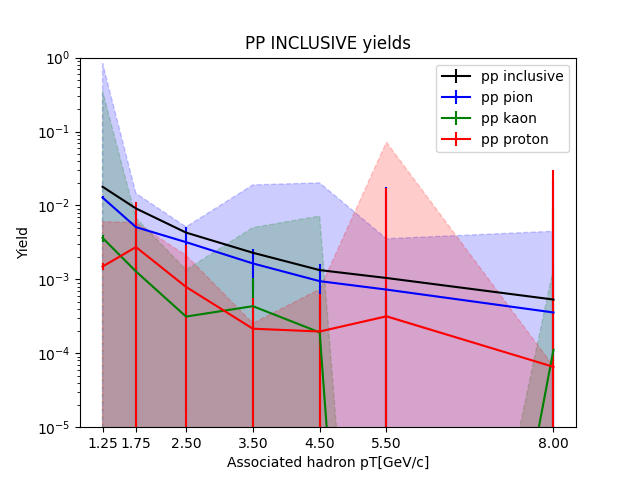
\includegraphics[width=\textwidth]{figures/png/appendix_plots/PP/Region.INCLUSIVE_yields.png}
                        \caption{Particle yields for PP INCLUSIVE region.}
                        \label{fig:appendix_PP_INCLUSIVE_Inclusive_Yields}
                    \end{subfigure}
                    \begin{subfigure}[b]{0.5\textwidth}
                        \centering
                        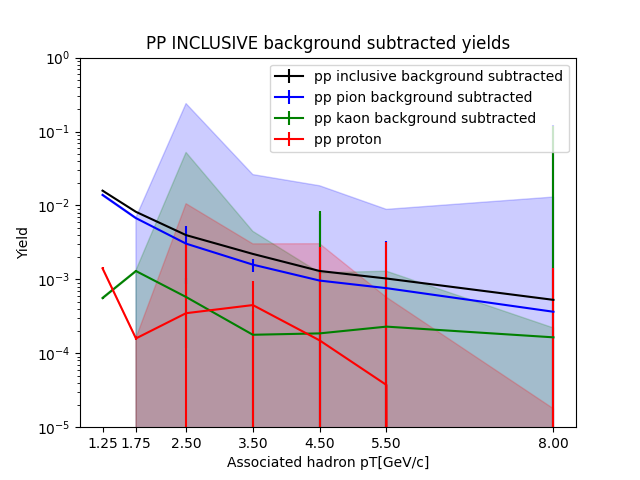
\includegraphics[width=\textwidth]{figures/png/appendix_plots/PP/Region.INCLUSIVE_background_subtracted_yields.png}
                        \caption{Particle yields for PP INCLUSIVE region with background subtracted.}
                        \label{fig:appendix_PP_INCLUSIVE_Inclusive_Yields_Background_Subtracted}
                    \end{subfigure}
                    \begin{subfigure}[b]{0.5\textwidth}
                        \centering
                        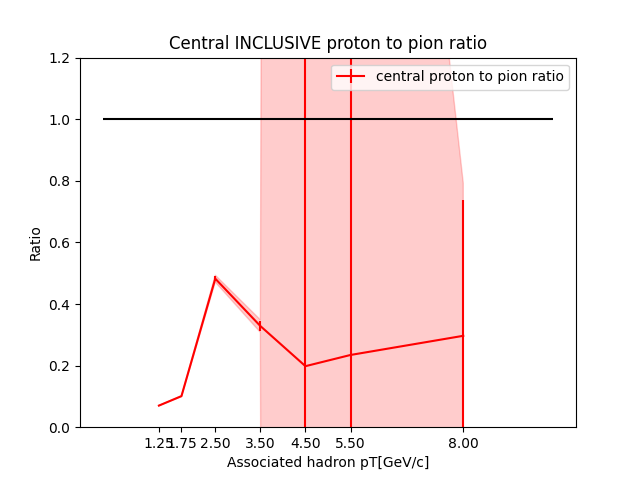
\includegraphics[width=\textwidth]{figures/png/appendix_plots/PP/Region.INCLUSIVE_proton_to_pion_ratio.png}
                        \caption{Proton to Pion ratio for PP INCLUSIVE region.}
                        \label{fig:appendix_PP_INCLUSIVE_Proton_to_Pion_Ratio}
                    \end{subfigure}
                    \begin{subfigure}[b]{0.5\textwidth}
                        \centering
                        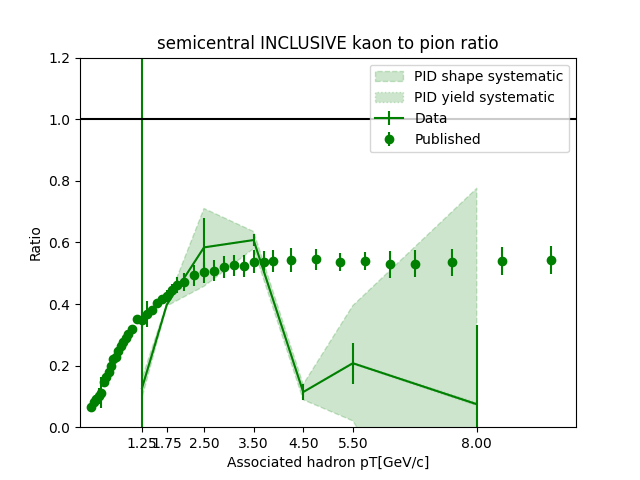
\includegraphics[width=\textwidth]{figures/png/appendix_plots/PP/Region.INCLUSIVE_kaon_to_pion_ratio.png}
                        \caption{Kaon to Pion ratio for PP INCLUSIVE region.}
                        \label{fig:appendix_PP_INCLUSIVE_Kaon_to_Pion_Ratio}
                    \end{subfigure}
                    \caption{Particle yields and ratios for PP INCLUSIVE region.}
                    \label{fig:appendix_PP_INCLUSIVE_Inclusive_Yields_and_Ratios}
                \end{figure}
                \begin{figure}[H]
                    \title{Region Near-side}
                    \begin{subfigure}[b]{0.5\textwidth}
                        \centering
                        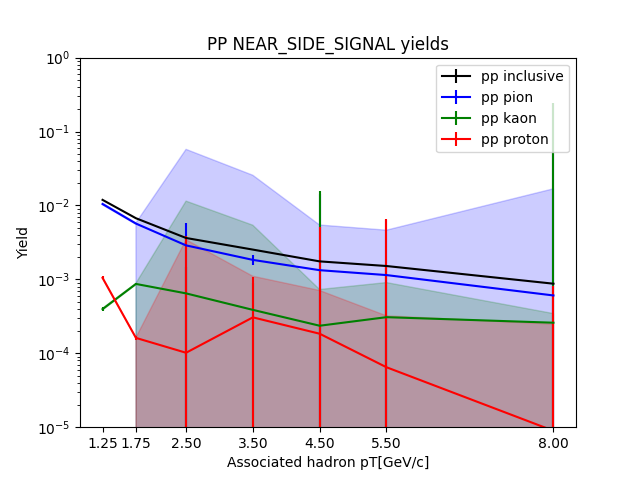
\includegraphics[width=\textwidth]{figures/png/appendix_plots/PP/Region.NEAR_SIDE_SIGNAL_yields.png}
                        \caption{Particle yields for PP NEAR-SIDE region.}
                        \label{fig:appendix_PP_NEAR_SIDE_SIGNAL_Inclusive_Yields}
                    \end{subfigure}
                    \begin{subfigure}[b]{0.5\textwidth}
                        \centering
                        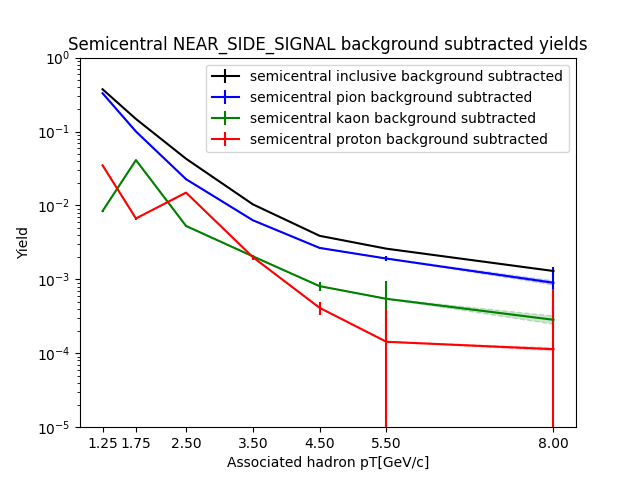
\includegraphics[width=\textwidth]{figures/png/appendix_plots/PP/Region.NEAR_SIDE_SIGNAL_background_subtracted_yields.png}
                        \caption{Particle yields for PP NEAR-SIDE region with background subtracted.}
                        \label{fig:appendix_PP_NEAR_SIDE_SIGNAL_Inclusive_Yields_Background_Subtracted}
                    \end{subfigure}
                    \begin{subfigure}[b]{0.5\textwidth}
                        \centering
                        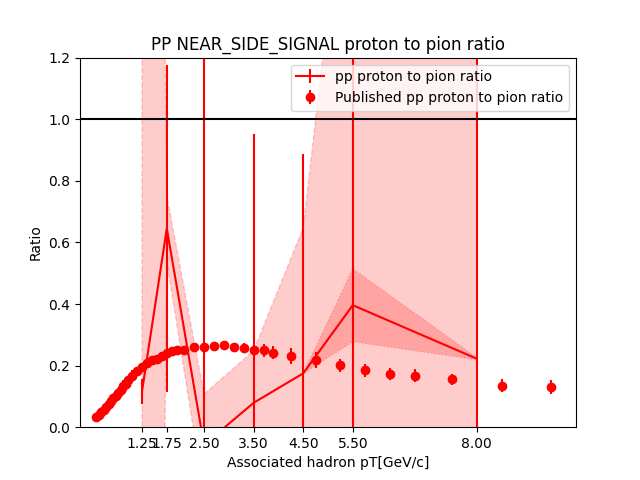
\includegraphics[width=\textwidth]{figures/png/appendix_plots/PP/Region.NEAR_SIDE_SIGNAL_proton_to_pion_ratio.png}
                        \caption{Proton to Pion ratio for PP NEAR-SIDE region.}
                        \label{fig:appendix_PP_NEAR_SIDE_SIGNAL_Proton_to_Pion_Ratio}
                    \end{subfigure}
                    \begin{subfigure}[b]{0.5\textwidth}
                        \centering
                        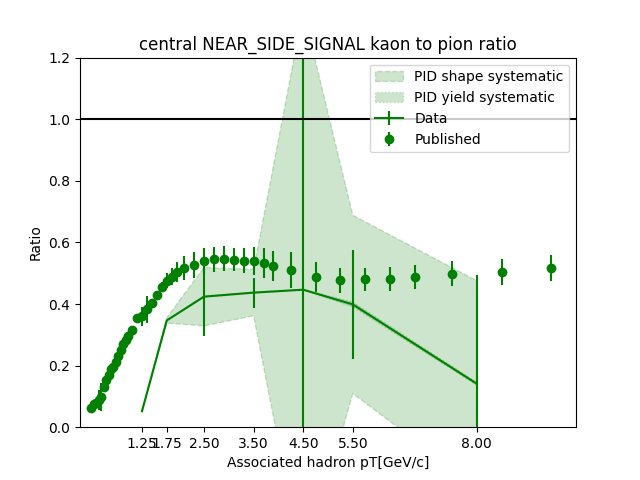
\includegraphics[width=\textwidth]{figures/png/appendix_plots/PP/Region.NEAR_SIDE_SIGNAL_kaon_to_pion_ratio.png}
                        \caption{Kaon to Pion ratio for PP NEAR-SIDE region.}
                        \label{fig:appendix_PP_NEAR_SIDE_SIGNAL_Kaon_to_Pion_Ratio}
                    \end{subfigure}
                    \caption{Particle yields and ratios for PP NEAR-SIDE region.}
                    \label{fig:appendix_PP_NEAR_SIDE_SIGNAL_Inclusive_Yields_and_Ratios}
                \end{figure}
                \begin{figure}[H]
                    \title{Region Away-side}
                    \begin{subfigure}[b]{0.5\textwidth}
                        \centering
                        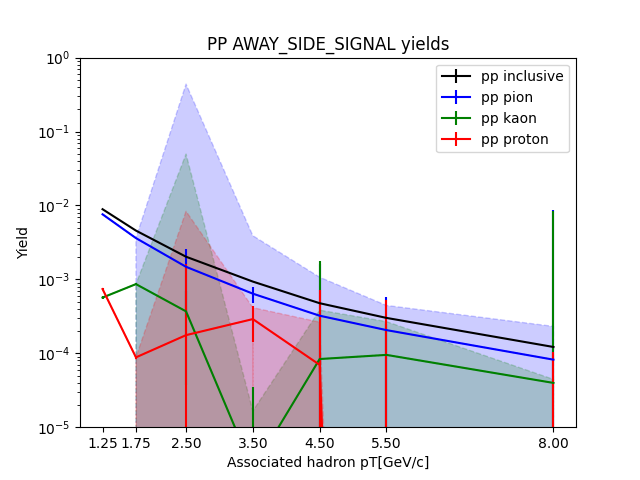
\includegraphics[width=\textwidth]{figures/png/appendix_plots/PP/Region.AWAY_SIDE_SIGNAL_yields.png}
                        \caption{Particle yields for PP AWAY-SIDE region.}
                        \label{fig:appendix_PP_AWAY_SIDE_SIGNAL_Inclusive_Yields}
                    \end{subfigure}
                    \begin{subfigure}[b]{0.5\textwidth}
                        \centering
                        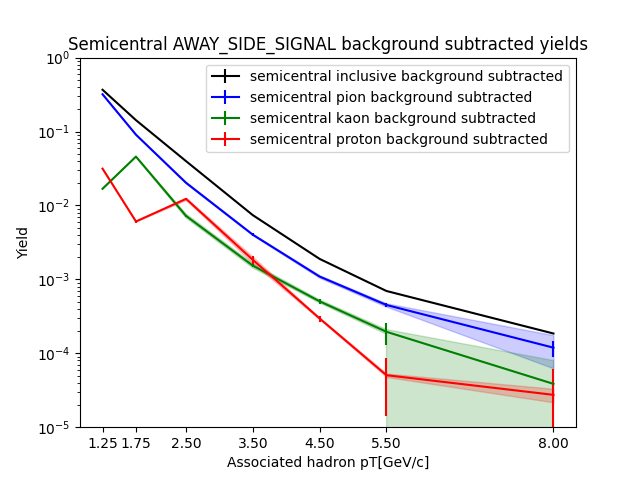
\includegraphics[width=\textwidth]{figures/png/appendix_plots/PP/Region.AWAY_SIDE_SIGNAL_background_subtracted_yields.png}
                        \caption{Particle yields for PP AWAY-SIDE region with background subtracted.}
                        \label{fig:appendix_PP_AWAY_SIDE_SIGNAL_Inclusive_Yields_Background_Subtracted}
                    \end{subfigure}
                    \begin{subfigure}[b]{0.5\textwidth}
                        \centering
                        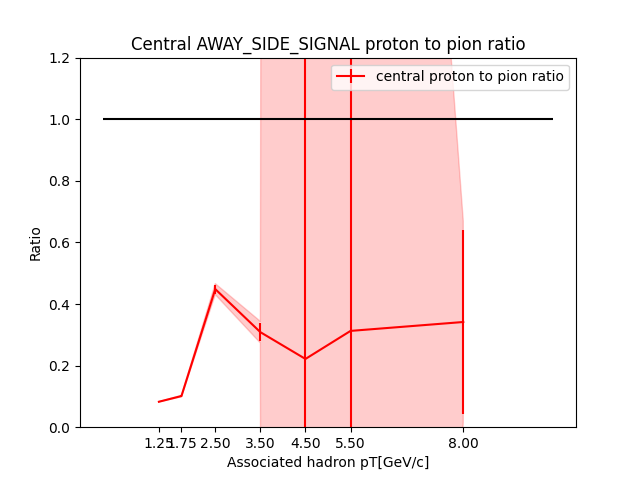
\includegraphics[width=\textwidth]{figures/png/appendix_plots/PP/Region.AWAY_SIDE_SIGNAL_proton_to_pion_ratio.png}
                        \caption{Proton to Pion ratio for PP AWAY-SIDE region.}
                        \label{fig:appendix_PP_AWAY_SIDE_SIGNAL_Proton_to_Pion_Ratio}
                    \end{subfigure}
                    \begin{subfigure}[b]{0.5\textwidth}
                        \centering
                        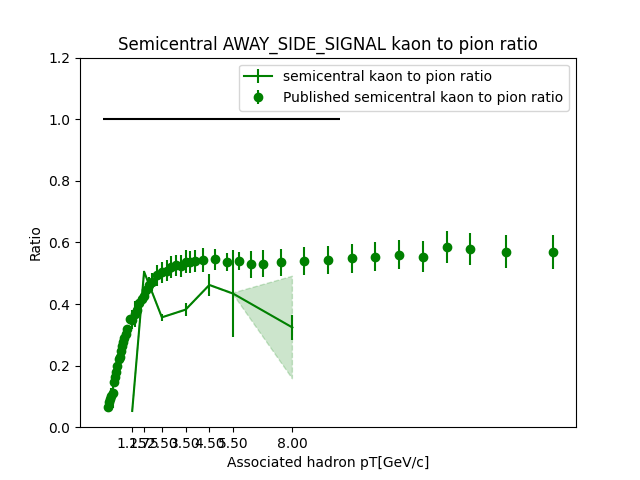
\includegraphics[width=\textwidth]{figures/png/appendix_plots/PP/Region.AWAY_SIDE_SIGNAL_kaon_to_pion_ratio.png}
                        \caption{Kaon to Pion ratio for PP AWAY-SIDE region.}
                        \label{fig:appendix_PP_AWAY_SIDE_SIGNAL_Kaon_to_Pion_Ratio}
                    \end{subfigure}
                    \caption{Particle yields and ratios for PP AWAY-SIDE region.}
                    \label{fig:appendix_PP_AWAY_SIDE_SIGNAL_Inclusive_Yields_and_Ratios}
                \end{figure}
                \begin{figure}[H]
                    \title{Region Background}
                    \begin{subfigure}[b]{0.5\textwidth}
                        \centering
                        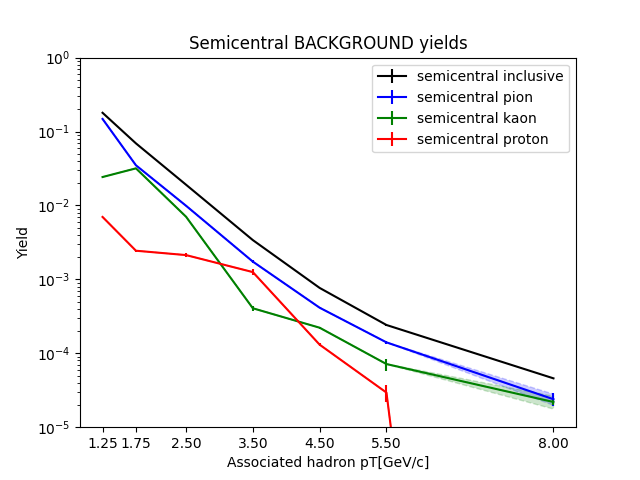
\includegraphics[width=\textwidth]{figures/png/appendix_plots/PP/Region.BACKGROUND_yields.png}
                        \caption{Particle yields for PP BACKGROUND region.}
                        \label{fig:appendix_PP_BACKGROUND_Inclusive_Yields}
                    \end{subfigure}
                    \caption{Particle yields for PP BACKGROUND region.}
                    \label{fig:appendix_PP_BACKGROUND_Inclusive_Yields}
                \end{figure}


    
            \subsection{PP PT-1-15}
            \begin{figure}[H]
                \title{Region Inclusive}
                \begin{subfigure}[b]{0.5\textwidth}
                    \centering
                    \includegraphics[width=\textwidth]{figures/png/appendix_plots/PP/PT_1_15/TPCnSigmaFits/TPCnSigmaFit_Region.INCLUSIVE_Inclusive.png}
                    \caption{TPC n$\sigma$ fits for PP PT-1-15 INCLUSIVE region for Inclusive particles.}
                    \label{fig:appendix_PP_PT-1-15_INCLUSIVE_Inclusive}
                \end{subfigure}
                \begin{subfigure}[b]{0.5\textwidth}
                    \centering
                    \includegraphics[width=\textwidth]{figures/png/appendix_plots/PP/PT_1_15/TPCnSigmaFits/TPCnSigmaFit_Region.INCLUSIVE_Pion.png}
                    \caption{TPC n$\sigma$ fits for PP PT-1-15 INCLUSIVE region for Pions.}
                    \label{fig:appendix_PP_PT-1-15_INCLUSIVE_Pion}
                \end{subfigure}
                \begin{subfigure}[b]{0.5\textwidth}
                    \centering
                    \includegraphics[width=\textwidth]{figures/png/appendix_plots/PP/PT_1_15/TPCnSigmaFits/TPCnSigmaFit_Region.INCLUSIVE_Proton.png}
                    \caption{TPC n$\sigma$ fits for PP PT-1-15 INCLUSIVE region for Protons.}
                    \label{fig:appendix_PP_PT-1-15_INCLUSIVE_Proton}
                \end{subfigure}
                \begin{subfigure}[b]{0.5\textwidth}
                    \centering
                    \includegraphics[width=\textwidth]{figures/png/appendix_plots/PP/PT_1_15/TPCnSigmaFits/TPCnSigmaFit_Region.INCLUSIVE_Kaon.png}
                    \caption{TPC n$\sigma$ fits for PP PT-1-15 INCLUSIVE region for Kaons.}
                    \label{fig:appendix_PP_PT-1-15_INCLUSIVE_Kaon}
                \end{subfigure}
                \caption{TPC n$\sigma$ fits for PP PT-1-15 INCLUSIVE region.}
                \label{fig:appendix_PP_PT-1-15_INCLUSIVE}
            \end{figure}
            \begin{figure}[H]
                \title{Region Near-side}
                \begin{subfigure}[b]{0.5\textwidth}
                    \centering
                    \includegraphics[width=\textwidth]{figures/png/appendix_plots/PP/PT_1_15/TPCnSigmaFits/TPCnSigmaFit_Region.NEAR_SIDE_SIGNAL_Inclusive.png}
                    \caption{TPC n$\sigma$ fits for PP PT-1-15 NEAR-SIDE region for Inclusive particles.}
                    \label{fig:appendix_PP_PT-1-15_NEAR_SIDE_SIGNAL_Inclusive}
                \end{subfigure}
                \begin{subfigure}[b]{0.5\textwidth}
                    \centering
                    \includegraphics[width=\textwidth]{figures/png/appendix_plots/PP/PT_1_15/TPCnSigmaFits/TPCnSigmaFit_Region.NEAR_SIDE_SIGNAL_Pion.png}
                    \caption{TPC n$\sigma$ fits for PP PT-1-15 NEAR-SIDE region for Pions.}
                    \label{fig:appendix_PP_PT-1-15_NEAR_SIDE_SIGNAL_Pion}
                \end{subfigure}
                \begin{subfigure}[b]{0.5\textwidth}
                    \centering
                    \includegraphics[width=\textwidth]{figures/png/appendix_plots/PP/PT_1_15/TPCnSigmaFits/TPCnSigmaFit_Region.NEAR_SIDE_SIGNAL_Proton.png}
                    \caption{TPC n$\sigma$ fits for PP PT-1-15 NEAR-SIDE region for Protons.}
                    \label{fig:appendix_PP_PT-1-15_NEAR_SIDE_SIGNAL_Proton}
                \end{subfigure}
                \begin{subfigure}[b]{0.5\textwidth}
                    \centering
                    \includegraphics[width=\textwidth]{figures/png/appendix_plots/PP/PT_1_15/TPCnSigmaFits/TPCnSigmaFit_Region.NEAR_SIDE_SIGNAL_Kaon.png}
                    \caption{TPC n$\sigma$ fits for PP PT-1-15 NEAR-SIDE region for Kaons.}
                    \label{fig:appendix_PP_PT-1-15_NEAR_SIDE_SIGNAL_Kaon}
                \end{subfigure}
                \caption{TPC n$\sigma$ fits for PP PT-1-15 NEAR-SIDE region.}
                \label{fig:appendix_PP_PT-1-15_NEAR_SIDE_SIGNAL}
            \end{figure}
            \begin{figure}[H]
                \title{Region Away-side}
                \begin{subfigure}[b]{0.5\textwidth}
                    \centering
                    \includegraphics[width=\textwidth]{figures/png/appendix_plots/PP/PT_1_15/TPCnSigmaFits/TPCnSigmaFit_Region.AWAY_SIDE_SIGNAL_Inclusive.png}
                    \caption{TPC n$\sigma$ fits for PP PT-1-15 AWAY-SIDE region for Inclusive particles.}
                    \label{fig:appendix_PP_PT-1-15_AWAY_SIDE_SIGNAL_Inclusive}
                \end{subfigure}
                \begin{subfigure}[b]{0.5\textwidth}
                    \centering
                    \includegraphics[width=\textwidth]{figures/png/appendix_plots/PP/PT_1_15/TPCnSigmaFits/TPCnSigmaFit_Region.AWAY_SIDE_SIGNAL_Pion.png}
                    \caption{TPC n$\sigma$ fits for PP PT-1-15 AWAY-SIDE region for Pions.}
                    \label{fig:appendix_PP_PT-1-15_AWAY_SIDE_SIGNAL_Pion}
                \end{subfigure}
                \begin{subfigure}[b]{0.5\textwidth}
                    \centering
                    \includegraphics[width=\textwidth]{figures/png/appendix_plots/PP/PT_1_15/TPCnSigmaFits/TPCnSigmaFit_Region.AWAY_SIDE_SIGNAL_Proton.png}
                    \caption{TPC n$\sigma$ fits for PP PT-1-15 AWAY-SIDE region for Protons.}
                    \label{fig:appendix_PP_PT-1-15_AWAY_SIDE_SIGNAL_Proton}
                \end{subfigure}
                \begin{subfigure}[b]{0.5\textwidth}
                    \centering
                    \includegraphics[width=\textwidth]{figures/png/appendix_plots/PP/PT_1_15/TPCnSigmaFits/TPCnSigmaFit_Region.AWAY_SIDE_SIGNAL_Kaon.png}
                    \caption{TPC n$\sigma$ fits for PP PT-1-15 AWAY-SIDE region for Kaons.}
                    \label{fig:appendix_PP_PT-1-15_AWAY_SIDE_SIGNAL_Kaon}
                \end{subfigure}
                \caption{TPC n$\sigma$ fits for PP PT-1-15 AWAY-SIDE region.}
                \label{fig:appendix_PP_PT-1-15_AWAY_SIDE_SIGNAL}
            \end{figure}
            \begin{figure}[H]
                \title{Region Background}
                \begin{subfigure}[b]{0.5\textwidth}
                    \centering
                    \includegraphics[width=\textwidth]{figures/png/appendix_plots/PP/PT_1_15/TPCnSigmaFits/TPCnSigmaFit_Region.BACKGROUND_Inclusive.png}
                    \caption{TPC n$\sigma$ fits for PP PT-1-15 BACKGROUND region for Inclusive particles.}
                    \label{fig:appendix_PP_PT-1-15_BACKGROUND_Inclusive}
                \end{subfigure}
                \begin{subfigure}[b]{0.5\textwidth}
                    \centering
                    \includegraphics[width=\textwidth]{figures/png/appendix_plots/PP/PT_1_15/TPCnSigmaFits/TPCnSigmaFit_Region.BACKGROUND_Pion.png}
                    \caption{TPC n$\sigma$ fits for PP PT-1-15 BACKGROUND region for Pions.}
                    \label{fig:appendix_PP_PT-1-15_BACKGROUND_Pion}
                \end{subfigure}
                \begin{subfigure}[b]{0.5\textwidth}
                    \centering
                    \includegraphics[width=\textwidth]{figures/png/appendix_plots/PP/PT_1_15/TPCnSigmaFits/TPCnSigmaFit_Region.BACKGROUND_Proton.png}
                    \caption{TPC n$\sigma$ fits for PP PT-1-15 BACKGROUND region for Protons.}
                    \label{fig:appendix_PP_PT-1-15_BACKGROUND_Proton}
                \end{subfigure}
                \begin{subfigure}[b]{0.5\textwidth}
                    \centering
                    \includegraphics[width=\textwidth]{figures/png/appendix_plots/PP/PT_1_15/TPCnSigmaFits/TPCnSigmaFit_Region.BACKGROUND_Kaon.png}
                    \caption{TPC n$\sigma$ fits for PP PT-1-15 BACKGROUND region for Kaons.}
                    \label{fig:appendix_PP_PT-1-15_BACKGROUND_Kaon}
                \end{subfigure}
                \caption{TPC n$\sigma$ fits for PP PT-1-15 BACKGROUND region.}
                \label{fig:appendix_PP_PT-1-15_BACKGROUND}
            \end{figure}
            \clearpage
            
    
            \subsection{PP PT-15-2}
            \begin{figure}[H]
                \title{Region Inclusive}
                \begin{subfigure}[b]{0.5\textwidth}
                    \centering
                    \includegraphics[width=\textwidth]{figures/png/appendix_plots/PP/PT_15_2/TPCnSigmaFits/TPCnSigmaFit_Region.INCLUSIVE_Inclusive.png}
                    \caption{TPC n$\sigma$ fits for PP PT-15-2 INCLUSIVE region for Inclusive particles.}
                    \label{fig:appendix_PP_PT-15-2_INCLUSIVE_Inclusive}
                \end{subfigure}
                \begin{subfigure}[b]{0.5\textwidth}
                    \centering
                    \includegraphics[width=\textwidth]{figures/png/appendix_plots/PP/PT_15_2/TPCnSigmaFits/TPCnSigmaFit_Region.INCLUSIVE_Pion.png}
                    \caption{TPC n$\sigma$ fits for PP PT-15-2 INCLUSIVE region for Pions.}
                    \label{fig:appendix_PP_PT-15-2_INCLUSIVE_Pion}
                \end{subfigure}
                \begin{subfigure}[b]{0.5\textwidth}
                    \centering
                    \includegraphics[width=\textwidth]{figures/png/appendix_plots/PP/PT_15_2/TPCnSigmaFits/TPCnSigmaFit_Region.INCLUSIVE_Proton.png}
                    \caption{TPC n$\sigma$ fits for PP PT-15-2 INCLUSIVE region for Protons.}
                    \label{fig:appendix_PP_PT-15-2_INCLUSIVE_Proton}
                \end{subfigure}
                \begin{subfigure}[b]{0.5\textwidth}
                    \centering
                    \includegraphics[width=\textwidth]{figures/png/appendix_plots/PP/PT_15_2/TPCnSigmaFits/TPCnSigmaFit_Region.INCLUSIVE_Kaon.png}
                    \caption{TPC n$\sigma$ fits for PP PT-15-2 INCLUSIVE region for Kaons.}
                    \label{fig:appendix_PP_PT-15-2_INCLUSIVE_Kaon}
                \end{subfigure}
                \caption{TPC n$\sigma$ fits for PP PT-15-2 INCLUSIVE region.}
                \label{fig:appendix_PP_PT-15-2_INCLUSIVE}
            \end{figure}
            \begin{figure}[H]
                \title{Region Near-side}
                \begin{subfigure}[b]{0.5\textwidth}
                    \centering
                    \includegraphics[width=\textwidth]{figures/png/appendix_plots/PP/PT_15_2/TPCnSigmaFits/TPCnSigmaFit_Region.NEAR_SIDE_SIGNAL_Inclusive.png}
                    \caption{TPC n$\sigma$ fits for PP PT-15-2 NEAR-SIDE region for Inclusive particles.}
                    \label{fig:appendix_PP_PT-15-2_NEAR_SIDE_SIGNAL_Inclusive}
                \end{subfigure}
                \begin{subfigure}[b]{0.5\textwidth}
                    \centering
                    \includegraphics[width=\textwidth]{figures/png/appendix_plots/PP/PT_15_2/TPCnSigmaFits/TPCnSigmaFit_Region.NEAR_SIDE_SIGNAL_Pion.png}
                    \caption{TPC n$\sigma$ fits for PP PT-15-2 NEAR-SIDE region for Pions.}
                    \label{fig:appendix_PP_PT-15-2_NEAR_SIDE_SIGNAL_Pion}
                \end{subfigure}
                \begin{subfigure}[b]{0.5\textwidth}
                    \centering
                    \includegraphics[width=\textwidth]{figures/png/appendix_plots/PP/PT_15_2/TPCnSigmaFits/TPCnSigmaFit_Region.NEAR_SIDE_SIGNAL_Proton.png}
                    \caption{TPC n$\sigma$ fits for PP PT-15-2 NEAR-SIDE region for Protons.}
                    \label{fig:appendix_PP_PT-15-2_NEAR_SIDE_SIGNAL_Proton}
                \end{subfigure}
                \begin{subfigure}[b]{0.5\textwidth}
                    \centering
                    \includegraphics[width=\textwidth]{figures/png/appendix_plots/PP/PT_15_2/TPCnSigmaFits/TPCnSigmaFit_Region.NEAR_SIDE_SIGNAL_Kaon.png}
                    \caption{TPC n$\sigma$ fits for PP PT-15-2 NEAR-SIDE region for Kaons.}
                    \label{fig:appendix_PP_PT-15-2_NEAR_SIDE_SIGNAL_Kaon}
                \end{subfigure}
                \caption{TPC n$\sigma$ fits for PP PT-15-2 NEAR-SIDE region.}
                \label{fig:appendix_PP_PT-15-2_NEAR_SIDE_SIGNAL}
            \end{figure}
            \begin{figure}[H]
                \title{Region Away-side}
                \begin{subfigure}[b]{0.5\textwidth}
                    \centering
                    \includegraphics[width=\textwidth]{figures/png/appendix_plots/PP/PT_15_2/TPCnSigmaFits/TPCnSigmaFit_Region.AWAY_SIDE_SIGNAL_Inclusive.png}
                    \caption{TPC n$\sigma$ fits for PP PT-15-2 AWAY-SIDE region for Inclusive particles.}
                    \label{fig:appendix_PP_PT-15-2_AWAY_SIDE_SIGNAL_Inclusive}
                \end{subfigure}
                \begin{subfigure}[b]{0.5\textwidth}
                    \centering
                    \includegraphics[width=\textwidth]{figures/png/appendix_plots/PP/PT_15_2/TPCnSigmaFits/TPCnSigmaFit_Region.AWAY_SIDE_SIGNAL_Pion.png}
                    \caption{TPC n$\sigma$ fits for PP PT-15-2 AWAY-SIDE region for Pions.}
                    \label{fig:appendix_PP_PT-15-2_AWAY_SIDE_SIGNAL_Pion}
                \end{subfigure}
                \begin{subfigure}[b]{0.5\textwidth}
                    \centering
                    \includegraphics[width=\textwidth]{figures/png/appendix_plots/PP/PT_15_2/TPCnSigmaFits/TPCnSigmaFit_Region.AWAY_SIDE_SIGNAL_Proton.png}
                    \caption{TPC n$\sigma$ fits for PP PT-15-2 AWAY-SIDE region for Protons.}
                    \label{fig:appendix_PP_PT-15-2_AWAY_SIDE_SIGNAL_Proton}
                \end{subfigure}
                \begin{subfigure}[b]{0.5\textwidth}
                    \centering
                    \includegraphics[width=\textwidth]{figures/png/appendix_plots/PP/PT_15_2/TPCnSigmaFits/TPCnSigmaFit_Region.AWAY_SIDE_SIGNAL_Kaon.png}
                    \caption{TPC n$\sigma$ fits for PP PT-15-2 AWAY-SIDE region for Kaons.}
                    \label{fig:appendix_PP_PT-15-2_AWAY_SIDE_SIGNAL_Kaon}
                \end{subfigure}
                \caption{TPC n$\sigma$ fits for PP PT-15-2 AWAY-SIDE region.}
                \label{fig:appendix_PP_PT-15-2_AWAY_SIDE_SIGNAL}
            \end{figure}
            \begin{figure}[H]
                \title{Region Background}
                \begin{subfigure}[b]{0.5\textwidth}
                    \centering
                    \includegraphics[width=\textwidth]{figures/png/appendix_plots/PP/PT_15_2/TPCnSigmaFits/TPCnSigmaFit_Region.BACKGROUND_Inclusive.png}
                    \caption{TPC n$\sigma$ fits for PP PT-15-2 BACKGROUND region for Inclusive particles.}
                    \label{fig:appendix_PP_PT-15-2_BACKGROUND_Inclusive}
                \end{subfigure}
                \begin{subfigure}[b]{0.5\textwidth}
                    \centering
                    \includegraphics[width=\textwidth]{figures/png/appendix_plots/PP/PT_15_2/TPCnSigmaFits/TPCnSigmaFit_Region.BACKGROUND_Pion.png}
                    \caption{TPC n$\sigma$ fits for PP PT-15-2 BACKGROUND region for Pions.}
                    \label{fig:appendix_PP_PT-15-2_BACKGROUND_Pion}
                \end{subfigure}
                \begin{subfigure}[b]{0.5\textwidth}
                    \centering
                    \includegraphics[width=\textwidth]{figures/png/appendix_plots/PP/PT_15_2/TPCnSigmaFits/TPCnSigmaFit_Region.BACKGROUND_Proton.png}
                    \caption{TPC n$\sigma$ fits for PP PT-15-2 BACKGROUND region for Protons.}
                    \label{fig:appendix_PP_PT-15-2_BACKGROUND_Proton}
                \end{subfigure}
                \begin{subfigure}[b]{0.5\textwidth}
                    \centering
                    \includegraphics[width=\textwidth]{figures/png/appendix_plots/PP/PT_15_2/TPCnSigmaFits/TPCnSigmaFit_Region.BACKGROUND_Kaon.png}
                    \caption{TPC n$\sigma$ fits for PP PT-15-2 BACKGROUND region for Kaons.}
                    \label{fig:appendix_PP_PT-15-2_BACKGROUND_Kaon}
                \end{subfigure}
                \caption{TPC n$\sigma$ fits for PP PT-15-2 BACKGROUND region.}
                \label{fig:appendix_PP_PT-15-2_BACKGROUND}
            \end{figure}
            \clearpage
            
    
            \subsection{PP PT-2-3}
            \begin{figure}[H]
                \title{Region Inclusive}
                \begin{subfigure}[b]{0.5\textwidth}
                    \centering
                    \includegraphics[width=\textwidth]{figures/png/appendix_plots/PP/PT_2_3/TPCnSigmaFits/TPCnSigmaFit_Region.INCLUSIVE_Inclusive.png}
                    \caption{TPC n$\sigma$ fits for PP PT-2-3 INCLUSIVE region for Inclusive particles.}
                    \label{fig:appendix_PP_PT-2-3_INCLUSIVE_Inclusive}
                \end{subfigure}
                \begin{subfigure}[b]{0.5\textwidth}
                    \centering
                    \includegraphics[width=\textwidth]{figures/png/appendix_plots/PP/PT_2_3/TPCnSigmaFits/TPCnSigmaFit_Region.INCLUSIVE_Pion.png}
                    \caption{TPC n$\sigma$ fits for PP PT-2-3 INCLUSIVE region for Pions.}
                    \label{fig:appendix_PP_PT-2-3_INCLUSIVE_Pion}
                \end{subfigure}
                \begin{subfigure}[b]{0.5\textwidth}
                    \centering
                    \includegraphics[width=\textwidth]{figures/png/appendix_plots/PP/PT_2_3/TPCnSigmaFits/TPCnSigmaFit_Region.INCLUSIVE_Proton.png}
                    \caption{TPC n$\sigma$ fits for PP PT-2-3 INCLUSIVE region for Protons.}
                    \label{fig:appendix_PP_PT-2-3_INCLUSIVE_Proton}
                \end{subfigure}
                \begin{subfigure}[b]{0.5\textwidth}
                    \centering
                    \includegraphics[width=\textwidth]{figures/png/appendix_plots/PP/PT_2_3/TPCnSigmaFits/TPCnSigmaFit_Region.INCLUSIVE_Kaon.png}
                    \caption{TPC n$\sigma$ fits for PP PT-2-3 INCLUSIVE region for Kaons.}
                    \label{fig:appendix_PP_PT-2-3_INCLUSIVE_Kaon}
                \end{subfigure}
                \caption{TPC n$\sigma$ fits for PP PT-2-3 INCLUSIVE region.}
                \label{fig:appendix_PP_PT-2-3_INCLUSIVE}
            \end{figure}
            \begin{figure}[H]
                \title{Region Near-side}
                \begin{subfigure}[b]{0.5\textwidth}
                    \centering
                    \includegraphics[width=\textwidth]{figures/png/appendix_plots/PP/PT_2_3/TPCnSigmaFits/TPCnSigmaFit_Region.NEAR_SIDE_SIGNAL_Inclusive.png}
                    \caption{TPC n$\sigma$ fits for PP PT-2-3 NEAR-SIDE region for Inclusive particles.}
                    \label{fig:appendix_PP_PT-2-3_NEAR_SIDE_SIGNAL_Inclusive}
                \end{subfigure}
                \begin{subfigure}[b]{0.5\textwidth}
                    \centering
                    \includegraphics[width=\textwidth]{figures/png/appendix_plots/PP/PT_2_3/TPCnSigmaFits/TPCnSigmaFit_Region.NEAR_SIDE_SIGNAL_Pion.png}
                    \caption{TPC n$\sigma$ fits for PP PT-2-3 NEAR-SIDE region for Pions.}
                    \label{fig:appendix_PP_PT-2-3_NEAR_SIDE_SIGNAL_Pion}
                \end{subfigure}
                \begin{subfigure}[b]{0.5\textwidth}
                    \centering
                    \includegraphics[width=\textwidth]{figures/png/appendix_plots/PP/PT_2_3/TPCnSigmaFits/TPCnSigmaFit_Region.NEAR_SIDE_SIGNAL_Proton.png}
                    \caption{TPC n$\sigma$ fits for PP PT-2-3 NEAR-SIDE region for Protons.}
                    \label{fig:appendix_PP_PT-2-3_NEAR_SIDE_SIGNAL_Proton}
                \end{subfigure}
                \begin{subfigure}[b]{0.5\textwidth}
                    \centering
                    \includegraphics[width=\textwidth]{figures/png/appendix_plots/PP/PT_2_3/TPCnSigmaFits/TPCnSigmaFit_Region.NEAR_SIDE_SIGNAL_Kaon.png}
                    \caption{TPC n$\sigma$ fits for PP PT-2-3 NEAR-SIDE region for Kaons.}
                    \label{fig:appendix_PP_PT-2-3_NEAR_SIDE_SIGNAL_Kaon}
                \end{subfigure}
                \caption{TPC n$\sigma$ fits for PP PT-2-3 NEAR-SIDE region.}
                \label{fig:appendix_PP_PT-2-3_NEAR_SIDE_SIGNAL}
            \end{figure}
            \begin{figure}[H]
                \title{Region Away-side}
                \begin{subfigure}[b]{0.5\textwidth}
                    \centering
                    \includegraphics[width=\textwidth]{figures/png/appendix_plots/PP/PT_2_3/TPCnSigmaFits/TPCnSigmaFit_Region.AWAY_SIDE_SIGNAL_Inclusive.png}
                    \caption{TPC n$\sigma$ fits for PP PT-2-3 AWAY-SIDE region for Inclusive particles.}
                    \label{fig:appendix_PP_PT-2-3_AWAY_SIDE_SIGNAL_Inclusive}
                \end{subfigure}
                \begin{subfigure}[b]{0.5\textwidth}
                    \centering
                    \includegraphics[width=\textwidth]{figures/png/appendix_plots/PP/PT_2_3/TPCnSigmaFits/TPCnSigmaFit_Region.AWAY_SIDE_SIGNAL_Pion.png}
                    \caption{TPC n$\sigma$ fits for PP PT-2-3 AWAY-SIDE region for Pions.}
                    \label{fig:appendix_PP_PT-2-3_AWAY_SIDE_SIGNAL_Pion}
                \end{subfigure}
                \begin{subfigure}[b]{0.5\textwidth}
                    \centering
                    \includegraphics[width=\textwidth]{figures/png/appendix_plots/PP/PT_2_3/TPCnSigmaFits/TPCnSigmaFit_Region.AWAY_SIDE_SIGNAL_Proton.png}
                    \caption{TPC n$\sigma$ fits for PP PT-2-3 AWAY-SIDE region for Protons.}
                    \label{fig:appendix_PP_PT-2-3_AWAY_SIDE_SIGNAL_Proton}
                \end{subfigure}
                \begin{subfigure}[b]{0.5\textwidth}
                    \centering
                    \includegraphics[width=\textwidth]{figures/png/appendix_plots/PP/PT_2_3/TPCnSigmaFits/TPCnSigmaFit_Region.AWAY_SIDE_SIGNAL_Kaon.png}
                    \caption{TPC n$\sigma$ fits for PP PT-2-3 AWAY-SIDE region for Kaons.}
                    \label{fig:appendix_PP_PT-2-3_AWAY_SIDE_SIGNAL_Kaon}
                \end{subfigure}
                \caption{TPC n$\sigma$ fits for PP PT-2-3 AWAY-SIDE region.}
                \label{fig:appendix_PP_PT-2-3_AWAY_SIDE_SIGNAL}
            \end{figure}
            \begin{figure}[H]
                \title{Region Background}
                \begin{subfigure}[b]{0.5\textwidth}
                    \centering
                    \includegraphics[width=\textwidth]{figures/png/appendix_plots/PP/PT_2_3/TPCnSigmaFits/TPCnSigmaFit_Region.BACKGROUND_Inclusive.png}
                    \caption{TPC n$\sigma$ fits for PP PT-2-3 BACKGROUND region for Inclusive particles.}
                    \label{fig:appendix_PP_PT-2-3_BACKGROUND_Inclusive}
                \end{subfigure}
                \begin{subfigure}[b]{0.5\textwidth}
                    \centering
                    \includegraphics[width=\textwidth]{figures/png/appendix_plots/PP/PT_2_3/TPCnSigmaFits/TPCnSigmaFit_Region.BACKGROUND_Pion.png}
                    \caption{TPC n$\sigma$ fits for PP PT-2-3 BACKGROUND region for Pions.}
                    \label{fig:appendix_PP_PT-2-3_BACKGROUND_Pion}
                \end{subfigure}
                \begin{subfigure}[b]{0.5\textwidth}
                    \centering
                    \includegraphics[width=\textwidth]{figures/png/appendix_plots/PP/PT_2_3/TPCnSigmaFits/TPCnSigmaFit_Region.BACKGROUND_Proton.png}
                    \caption{TPC n$\sigma$ fits for PP PT-2-3 BACKGROUND region for Protons.}
                    \label{fig:appendix_PP_PT-2-3_BACKGROUND_Proton}
                \end{subfigure}
                \begin{subfigure}[b]{0.5\textwidth}
                    \centering
                    \includegraphics[width=\textwidth]{figures/png/appendix_plots/PP/PT_2_3/TPCnSigmaFits/TPCnSigmaFit_Region.BACKGROUND_Kaon.png}
                    \caption{TPC n$\sigma$ fits for PP PT-2-3 BACKGROUND region for Kaons.}
                    \label{fig:appendix_PP_PT-2-3_BACKGROUND_Kaon}
                \end{subfigure}
                \caption{TPC n$\sigma$ fits for PP PT-2-3 BACKGROUND region.}
                \label{fig:appendix_PP_PT-2-3_BACKGROUND}
            \end{figure}
            \clearpage
            
    
            \subsection{PP PT-3-4}
            \begin{figure}[H]
                \title{Region Inclusive}
                \begin{subfigure}[b]{0.5\textwidth}
                    \centering
                    \includegraphics[width=\textwidth]{figures/png/appendix_plots/PP/PT_3_4/TPCnSigmaFits/TPCnSigmaFit_Region.INCLUSIVE_Inclusive.png}
                    \caption{TPC n$\sigma$ fits for PP PT-3-4 INCLUSIVE region for Inclusive particles.}
                    \label{fig:appendix_PP_PT-3-4_INCLUSIVE_Inclusive}
                \end{subfigure}
                \begin{subfigure}[b]{0.5\textwidth}
                    \centering
                    \includegraphics[width=\textwidth]{figures/png/appendix_plots/PP/PT_3_4/TPCnSigmaFits/TPCnSigmaFit_Region.INCLUSIVE_Pion.png}
                    \caption{TPC n$\sigma$ fits for PP PT-3-4 INCLUSIVE region for Pions.}
                    \label{fig:appendix_PP_PT-3-4_INCLUSIVE_Pion}
                \end{subfigure}
                \begin{subfigure}[b]{0.5\textwidth}
                    \centering
                    \includegraphics[width=\textwidth]{figures/png/appendix_plots/PP/PT_3_4/TPCnSigmaFits/TPCnSigmaFit_Region.INCLUSIVE_Proton.png}
                    \caption{TPC n$\sigma$ fits for PP PT-3-4 INCLUSIVE region for Protons.}
                    \label{fig:appendix_PP_PT-3-4_INCLUSIVE_Proton}
                \end{subfigure}
                \begin{subfigure}[b]{0.5\textwidth}
                    \centering
                    \includegraphics[width=\textwidth]{figures/png/appendix_plots/PP/PT_3_4/TPCnSigmaFits/TPCnSigmaFit_Region.INCLUSIVE_Kaon.png}
                    \caption{TPC n$\sigma$ fits for PP PT-3-4 INCLUSIVE region for Kaons.}
                    \label{fig:appendix_PP_PT-3-4_INCLUSIVE_Kaon}
                \end{subfigure}
                \caption{TPC n$\sigma$ fits for PP PT-3-4 INCLUSIVE region.}
                \label{fig:appendix_PP_PT-3-4_INCLUSIVE}
            \end{figure}
            \begin{figure}[H]
                \title{Region Near-side}
                \begin{subfigure}[b]{0.5\textwidth}
                    \centering
                    \includegraphics[width=\textwidth]{figures/png/appendix_plots/PP/PT_3_4/TPCnSigmaFits/TPCnSigmaFit_Region.NEAR_SIDE_SIGNAL_Inclusive.png}
                    \caption{TPC n$\sigma$ fits for PP PT-3-4 NEAR-SIDE region for Inclusive particles.}
                    \label{fig:appendix_PP_PT-3-4_NEAR_SIDE_SIGNAL_Inclusive}
                \end{subfigure}
                \begin{subfigure}[b]{0.5\textwidth}
                    \centering
                    \includegraphics[width=\textwidth]{figures/png/appendix_plots/PP/PT_3_4/TPCnSigmaFits/TPCnSigmaFit_Region.NEAR_SIDE_SIGNAL_Pion.png}
                    \caption{TPC n$\sigma$ fits for PP PT-3-4 NEAR-SIDE region for Pions.}
                    \label{fig:appendix_PP_PT-3-4_NEAR_SIDE_SIGNAL_Pion}
                \end{subfigure}
                \begin{subfigure}[b]{0.5\textwidth}
                    \centering
                    \includegraphics[width=\textwidth]{figures/png/appendix_plots/PP/PT_3_4/TPCnSigmaFits/TPCnSigmaFit_Region.NEAR_SIDE_SIGNAL_Proton.png}
                    \caption{TPC n$\sigma$ fits for PP PT-3-4 NEAR-SIDE region for Protons.}
                    \label{fig:appendix_PP_PT-3-4_NEAR_SIDE_SIGNAL_Proton}
                \end{subfigure}
                \begin{subfigure}[b]{0.5\textwidth}
                    \centering
                    \includegraphics[width=\textwidth]{figures/png/appendix_plots/PP/PT_3_4/TPCnSigmaFits/TPCnSigmaFit_Region.NEAR_SIDE_SIGNAL_Kaon.png}
                    \caption{TPC n$\sigma$ fits for PP PT-3-4 NEAR-SIDE region for Kaons.}
                    \label{fig:appendix_PP_PT-3-4_NEAR_SIDE_SIGNAL_Kaon}
                \end{subfigure}
                \caption{TPC n$\sigma$ fits for PP PT-3-4 NEAR-SIDE region.}
                \label{fig:appendix_PP_PT-3-4_NEAR_SIDE_SIGNAL}
            \end{figure}
            \begin{figure}[H]
                \title{Region Away-side}
                \begin{subfigure}[b]{0.5\textwidth}
                    \centering
                    \includegraphics[width=\textwidth]{figures/png/appendix_plots/PP/PT_3_4/TPCnSigmaFits/TPCnSigmaFit_Region.AWAY_SIDE_SIGNAL_Inclusive.png}
                    \caption{TPC n$\sigma$ fits for PP PT-3-4 AWAY-SIDE region for Inclusive particles.}
                    \label{fig:appendix_PP_PT-3-4_AWAY_SIDE_SIGNAL_Inclusive}
                \end{subfigure}
                \begin{subfigure}[b]{0.5\textwidth}
                    \centering
                    \includegraphics[width=\textwidth]{figures/png/appendix_plots/PP/PT_3_4/TPCnSigmaFits/TPCnSigmaFit_Region.AWAY_SIDE_SIGNAL_Pion.png}
                    \caption{TPC n$\sigma$ fits for PP PT-3-4 AWAY-SIDE region for Pions.}
                    \label{fig:appendix_PP_PT-3-4_AWAY_SIDE_SIGNAL_Pion}
                \end{subfigure}
                \begin{subfigure}[b]{0.5\textwidth}
                    \centering
                    \includegraphics[width=\textwidth]{figures/png/appendix_plots/PP/PT_3_4/TPCnSigmaFits/TPCnSigmaFit_Region.AWAY_SIDE_SIGNAL_Proton.png}
                    \caption{TPC n$\sigma$ fits for PP PT-3-4 AWAY-SIDE region for Protons.}
                    \label{fig:appendix_PP_PT-3-4_AWAY_SIDE_SIGNAL_Proton}
                \end{subfigure}
                \begin{subfigure}[b]{0.5\textwidth}
                    \centering
                    \includegraphics[width=\textwidth]{figures/png/appendix_plots/PP/PT_3_4/TPCnSigmaFits/TPCnSigmaFit_Region.AWAY_SIDE_SIGNAL_Kaon.png}
                    \caption{TPC n$\sigma$ fits for PP PT-3-4 AWAY-SIDE region for Kaons.}
                    \label{fig:appendix_PP_PT-3-4_AWAY_SIDE_SIGNAL_Kaon}
                \end{subfigure}
                \caption{TPC n$\sigma$ fits for PP PT-3-4 AWAY-SIDE region.}
                \label{fig:appendix_PP_PT-3-4_AWAY_SIDE_SIGNAL}
            \end{figure}
            \begin{figure}[H]
                \title{Region Background}
                \begin{subfigure}[b]{0.5\textwidth}
                    \centering
                    \includegraphics[width=\textwidth]{figures/png/appendix_plots/PP/PT_3_4/TPCnSigmaFits/TPCnSigmaFit_Region.BACKGROUND_Inclusive.png}
                    \caption{TPC n$\sigma$ fits for PP PT-3-4 BACKGROUND region for Inclusive particles.}
                    \label{fig:appendix_PP_PT-3-4_BACKGROUND_Inclusive}
                \end{subfigure}
                \begin{subfigure}[b]{0.5\textwidth}
                    \centering
                    \includegraphics[width=\textwidth]{figures/png/appendix_plots/PP/PT_3_4/TPCnSigmaFits/TPCnSigmaFit_Region.BACKGROUND_Pion.png}
                    \caption{TPC n$\sigma$ fits for PP PT-3-4 BACKGROUND region for Pions.}
                    \label{fig:appendix_PP_PT-3-4_BACKGROUND_Pion}
                \end{subfigure}
                \begin{subfigure}[b]{0.5\textwidth}
                    \centering
                    \includegraphics[width=\textwidth]{figures/png/appendix_plots/PP/PT_3_4/TPCnSigmaFits/TPCnSigmaFit_Region.BACKGROUND_Proton.png}
                    \caption{TPC n$\sigma$ fits for PP PT-3-4 BACKGROUND region for Protons.}
                    \label{fig:appendix_PP_PT-3-4_BACKGROUND_Proton}
                \end{subfigure}
                \begin{subfigure}[b]{0.5\textwidth}
                    \centering
                    \includegraphics[width=\textwidth]{figures/png/appendix_plots/PP/PT_3_4/TPCnSigmaFits/TPCnSigmaFit_Region.BACKGROUND_Kaon.png}
                    \caption{TPC n$\sigma$ fits for PP PT-3-4 BACKGROUND region for Kaons.}
                    \label{fig:appendix_PP_PT-3-4_BACKGROUND_Kaon}
                \end{subfigure}
                \caption{TPC n$\sigma$ fits for PP PT-3-4 BACKGROUND region.}
                \label{fig:appendix_PP_PT-3-4_BACKGROUND}
            \end{figure}
            \clearpage
            
    
            \subsection{PP PT-4-5}
            \begin{figure}[H]
                \title{Region Inclusive}
                \begin{subfigure}[b]{0.5\textwidth}
                    \centering
                    \includegraphics[width=\textwidth]{figures/png/appendix_plots/PP/PT_4_5/TPCnSigmaFits/TPCnSigmaFit_Region.INCLUSIVE_Inclusive.png}
                    \caption{TPC n$\sigma$ fits for PP PT-4-5 INCLUSIVE region for Inclusive particles.}
                    \label{fig:appendix_PP_PT-4-5_INCLUSIVE_Inclusive}
                \end{subfigure}
                \begin{subfigure}[b]{0.5\textwidth}
                    \centering
                    \includegraphics[width=\textwidth]{figures/png/appendix_plots/PP/PT_4_5/TPCnSigmaFits/TPCnSigmaFit_Region.INCLUSIVE_Pion.png}
                    \caption{TPC n$\sigma$ fits for PP PT-4-5 INCLUSIVE region for Pions.}
                    \label{fig:appendix_PP_PT-4-5_INCLUSIVE_Pion}
                \end{subfigure}
                \begin{subfigure}[b]{0.5\textwidth}
                    \centering
                    \includegraphics[width=\textwidth]{figures/png/appendix_plots/PP/PT_4_5/TPCnSigmaFits/TPCnSigmaFit_Region.INCLUSIVE_Proton.png}
                    \caption{TPC n$\sigma$ fits for PP PT-4-5 INCLUSIVE region for Protons.}
                    \label{fig:appendix_PP_PT-4-5_INCLUSIVE_Proton}
                \end{subfigure}
                \begin{subfigure}[b]{0.5\textwidth}
                    \centering
                    \includegraphics[width=\textwidth]{figures/png/appendix_plots/PP/PT_4_5/TPCnSigmaFits/TPCnSigmaFit_Region.INCLUSIVE_Kaon.png}
                    \caption{TPC n$\sigma$ fits for PP PT-4-5 INCLUSIVE region for Kaons.}
                    \label{fig:appendix_PP_PT-4-5_INCLUSIVE_Kaon}
                \end{subfigure}
                \caption{TPC n$\sigma$ fits for PP PT-4-5 INCLUSIVE region.}
                \label{fig:appendix_PP_PT-4-5_INCLUSIVE}
            \end{figure}
            \begin{figure}[H]
                \title{Region Near-side}
                \begin{subfigure}[b]{0.5\textwidth}
                    \centering
                    \includegraphics[width=\textwidth]{figures/png/appendix_plots/PP/PT_4_5/TPCnSigmaFits/TPCnSigmaFit_Region.NEAR_SIDE_SIGNAL_Inclusive.png}
                    \caption{TPC n$\sigma$ fits for PP PT-4-5 NEAR-SIDE region for Inclusive particles.}
                    \label{fig:appendix_PP_PT-4-5_NEAR_SIDE_SIGNAL_Inclusive}
                \end{subfigure}
                \begin{subfigure}[b]{0.5\textwidth}
                    \centering
                    \includegraphics[width=\textwidth]{figures/png/appendix_plots/PP/PT_4_5/TPCnSigmaFits/TPCnSigmaFit_Region.NEAR_SIDE_SIGNAL_Pion.png}
                    \caption{TPC n$\sigma$ fits for PP PT-4-5 NEAR-SIDE region for Pions.}
                    \label{fig:appendix_PP_PT-4-5_NEAR_SIDE_SIGNAL_Pion}
                \end{subfigure}
                \begin{subfigure}[b]{0.5\textwidth}
                    \centering
                    \includegraphics[width=\textwidth]{figures/png/appendix_plots/PP/PT_4_5/TPCnSigmaFits/TPCnSigmaFit_Region.NEAR_SIDE_SIGNAL_Proton.png}
                    \caption{TPC n$\sigma$ fits for PP PT-4-5 NEAR-SIDE region for Protons.}
                    \label{fig:appendix_PP_PT-4-5_NEAR_SIDE_SIGNAL_Proton}
                \end{subfigure}
                \begin{subfigure}[b]{0.5\textwidth}
                    \centering
                    \includegraphics[width=\textwidth]{figures/png/appendix_plots/PP/PT_4_5/TPCnSigmaFits/TPCnSigmaFit_Region.NEAR_SIDE_SIGNAL_Kaon.png}
                    \caption{TPC n$\sigma$ fits for PP PT-4-5 NEAR-SIDE region for Kaons.}
                    \label{fig:appendix_PP_PT-4-5_NEAR_SIDE_SIGNAL_Kaon}
                \end{subfigure}
                \caption{TPC n$\sigma$ fits for PP PT-4-5 NEAR-SIDE region.}
                \label{fig:appendix_PP_PT-4-5_NEAR_SIDE_SIGNAL}
            \end{figure}
            \begin{figure}[H]
                \title{Region Away-side}
                \begin{subfigure}[b]{0.5\textwidth}
                    \centering
                    \includegraphics[width=\textwidth]{figures/png/appendix_plots/PP/PT_4_5/TPCnSigmaFits/TPCnSigmaFit_Region.AWAY_SIDE_SIGNAL_Inclusive.png}
                    \caption{TPC n$\sigma$ fits for PP PT-4-5 AWAY-SIDE region for Inclusive particles.}
                    \label{fig:appendix_PP_PT-4-5_AWAY_SIDE_SIGNAL_Inclusive}
                \end{subfigure}
                \begin{subfigure}[b]{0.5\textwidth}
                    \centering
                    \includegraphics[width=\textwidth]{figures/png/appendix_plots/PP/PT_4_5/TPCnSigmaFits/TPCnSigmaFit_Region.AWAY_SIDE_SIGNAL_Pion.png}
                    \caption{TPC n$\sigma$ fits for PP PT-4-5 AWAY-SIDE region for Pions.}
                    \label{fig:appendix_PP_PT-4-5_AWAY_SIDE_SIGNAL_Pion}
                \end{subfigure}
                \begin{subfigure}[b]{0.5\textwidth}
                    \centering
                    \includegraphics[width=\textwidth]{figures/png/appendix_plots/PP/PT_4_5/TPCnSigmaFits/TPCnSigmaFit_Region.AWAY_SIDE_SIGNAL_Proton.png}
                    \caption{TPC n$\sigma$ fits for PP PT-4-5 AWAY-SIDE region for Protons.}
                    \label{fig:appendix_PP_PT-4-5_AWAY_SIDE_SIGNAL_Proton}
                \end{subfigure}
                \begin{subfigure}[b]{0.5\textwidth}
                    \centering
                    \includegraphics[width=\textwidth]{figures/png/appendix_plots/PP/PT_4_5/TPCnSigmaFits/TPCnSigmaFit_Region.AWAY_SIDE_SIGNAL_Kaon.png}
                    \caption{TPC n$\sigma$ fits for PP PT-4-5 AWAY-SIDE region for Kaons.}
                    \label{fig:appendix_PP_PT-4-5_AWAY_SIDE_SIGNAL_Kaon}
                \end{subfigure}
                \caption{TPC n$\sigma$ fits for PP PT-4-5 AWAY-SIDE region.}
                \label{fig:appendix_PP_PT-4-5_AWAY_SIDE_SIGNAL}
            \end{figure}
            \begin{figure}[H]
                \title{Region Background}
                \begin{subfigure}[b]{0.5\textwidth}
                    \centering
                    \includegraphics[width=\textwidth]{figures/png/appendix_plots/PP/PT_4_5/TPCnSigmaFits/TPCnSigmaFit_Region.BACKGROUND_Inclusive.png}
                    \caption{TPC n$\sigma$ fits for PP PT-4-5 BACKGROUND region for Inclusive particles.}
                    \label{fig:appendix_PP_PT-4-5_BACKGROUND_Inclusive}
                \end{subfigure}
                \begin{subfigure}[b]{0.5\textwidth}
                    \centering
                    \includegraphics[width=\textwidth]{figures/png/appendix_plots/PP/PT_4_5/TPCnSigmaFits/TPCnSigmaFit_Region.BACKGROUND_Pion.png}
                    \caption{TPC n$\sigma$ fits for PP PT-4-5 BACKGROUND region for Pions.}
                    \label{fig:appendix_PP_PT-4-5_BACKGROUND_Pion}
                \end{subfigure}
                \begin{subfigure}[b]{0.5\textwidth}
                    \centering
                    \includegraphics[width=\textwidth]{figures/png/appendix_plots/PP/PT_4_5/TPCnSigmaFits/TPCnSigmaFit_Region.BACKGROUND_Proton.png}
                    \caption{TPC n$\sigma$ fits for PP PT-4-5 BACKGROUND region for Protons.}
                    \label{fig:appendix_PP_PT-4-5_BACKGROUND_Proton}
                \end{subfigure}
                \begin{subfigure}[b]{0.5\textwidth}
                    \centering
                    \includegraphics[width=\textwidth]{figures/png/appendix_plots/PP/PT_4_5/TPCnSigmaFits/TPCnSigmaFit_Region.BACKGROUND_Kaon.png}
                    \caption{TPC n$\sigma$ fits for PP PT-4-5 BACKGROUND region for Kaons.}
                    \label{fig:appendix_PP_PT-4-5_BACKGROUND_Kaon}
                \end{subfigure}
                \caption{TPC n$\sigma$ fits for PP PT-4-5 BACKGROUND region.}
                \label{fig:appendix_PP_PT-4-5_BACKGROUND}
            \end{figure}
            \clearpage
            
    
            \subsection{PP PT-5-6}
            \begin{figure}[H]
                \title{Region Inclusive}
                \begin{subfigure}[b]{0.5\textwidth}
                    \centering
                    \includegraphics[width=\textwidth]{figures/png/appendix_plots/PP/PT_5_6/TPCnSigmaFits/TPCnSigmaFit_Region.INCLUSIVE_Inclusive.png}
                    \caption{TPC n$\sigma$ fits for PP PT-5-6 INCLUSIVE region for Inclusive particles.}
                    \label{fig:appendix_PP_PT-5-6_INCLUSIVE_Inclusive}
                \end{subfigure}
                \begin{subfigure}[b]{0.5\textwidth}
                    \centering
                    \includegraphics[width=\textwidth]{figures/png/appendix_plots/PP/PT_5_6/TPCnSigmaFits/TPCnSigmaFit_Region.INCLUSIVE_Pion.png}
                    \caption{TPC n$\sigma$ fits for PP PT-5-6 INCLUSIVE region for Pions.}
                    \label{fig:appendix_PP_PT-5-6_INCLUSIVE_Pion}
                \end{subfigure}
                \begin{subfigure}[b]{0.5\textwidth}
                    \centering
                    \includegraphics[width=\textwidth]{figures/png/appendix_plots/PP/PT_5_6/TPCnSigmaFits/TPCnSigmaFit_Region.INCLUSIVE_Proton.png}
                    \caption{TPC n$\sigma$ fits for PP PT-5-6 INCLUSIVE region for Protons.}
                    \label{fig:appendix_PP_PT-5-6_INCLUSIVE_Proton}
                \end{subfigure}
                \begin{subfigure}[b]{0.5\textwidth}
                    \centering
                    \includegraphics[width=\textwidth]{figures/png/appendix_plots/PP/PT_5_6/TPCnSigmaFits/TPCnSigmaFit_Region.INCLUSIVE_Kaon.png}
                    \caption{TPC n$\sigma$ fits for PP PT-5-6 INCLUSIVE region for Kaons.}
                    \label{fig:appendix_PP_PT-5-6_INCLUSIVE_Kaon}
                \end{subfigure}
                \caption{TPC n$\sigma$ fits for PP PT-5-6 INCLUSIVE region.}
                \label{fig:appendix_PP_PT-5-6_INCLUSIVE}
            \end{figure}
            \begin{figure}[H]
                \title{Region Near-side}
                \begin{subfigure}[b]{0.5\textwidth}
                    \centering
                    \includegraphics[width=\textwidth]{figures/png/appendix_plots/PP/PT_5_6/TPCnSigmaFits/TPCnSigmaFit_Region.NEAR_SIDE_SIGNAL_Inclusive.png}
                    \caption{TPC n$\sigma$ fits for PP PT-5-6 NEAR-SIDE region for Inclusive particles.}
                    \label{fig:appendix_PP_PT-5-6_NEAR_SIDE_SIGNAL_Inclusive}
                \end{subfigure}
                \begin{subfigure}[b]{0.5\textwidth}
                    \centering
                    \includegraphics[width=\textwidth]{figures/png/appendix_plots/PP/PT_5_6/TPCnSigmaFits/TPCnSigmaFit_Region.NEAR_SIDE_SIGNAL_Pion.png}
                    \caption{TPC n$\sigma$ fits for PP PT-5-6 NEAR-SIDE region for Pions.}
                    \label{fig:appendix_PP_PT-5-6_NEAR_SIDE_SIGNAL_Pion}
                \end{subfigure}
                \begin{subfigure}[b]{0.5\textwidth}
                    \centering
                    \includegraphics[width=\textwidth]{figures/png/appendix_plots/PP/PT_5_6/TPCnSigmaFits/TPCnSigmaFit_Region.NEAR_SIDE_SIGNAL_Proton.png}
                    \caption{TPC n$\sigma$ fits for PP PT-5-6 NEAR-SIDE region for Protons.}
                    \label{fig:appendix_PP_PT-5-6_NEAR_SIDE_SIGNAL_Proton}
                \end{subfigure}
                \begin{subfigure}[b]{0.5\textwidth}
                    \centering
                    \includegraphics[width=\textwidth]{figures/png/appendix_plots/PP/PT_5_6/TPCnSigmaFits/TPCnSigmaFit_Region.NEAR_SIDE_SIGNAL_Kaon.png}
                    \caption{TPC n$\sigma$ fits for PP PT-5-6 NEAR-SIDE region for Kaons.}
                    \label{fig:appendix_PP_PT-5-6_NEAR_SIDE_SIGNAL_Kaon}
                \end{subfigure}
                \caption{TPC n$\sigma$ fits for PP PT-5-6 NEAR-SIDE region.}
                \label{fig:appendix_PP_PT-5-6_NEAR_SIDE_SIGNAL}
            \end{figure}
            \begin{figure}[H]
                \title{Region Away-side}
                \begin{subfigure}[b]{0.5\textwidth}
                    \centering
                    \includegraphics[width=\textwidth]{figures/png/appendix_plots/PP/PT_5_6/TPCnSigmaFits/TPCnSigmaFit_Region.AWAY_SIDE_SIGNAL_Inclusive.png}
                    \caption{TPC n$\sigma$ fits for PP PT-5-6 AWAY-SIDE region for Inclusive particles.}
                    \label{fig:appendix_PP_PT-5-6_AWAY_SIDE_SIGNAL_Inclusive}
                \end{subfigure}
                \begin{subfigure}[b]{0.5\textwidth}
                    \centering
                    \includegraphics[width=\textwidth]{figures/png/appendix_plots/PP/PT_5_6/TPCnSigmaFits/TPCnSigmaFit_Region.AWAY_SIDE_SIGNAL_Pion.png}
                    \caption{TPC n$\sigma$ fits for PP PT-5-6 AWAY-SIDE region for Pions.}
                    \label{fig:appendix_PP_PT-5-6_AWAY_SIDE_SIGNAL_Pion}
                \end{subfigure}
                \begin{subfigure}[b]{0.5\textwidth}
                    \centering
                    \includegraphics[width=\textwidth]{figures/png/appendix_plots/PP/PT_5_6/TPCnSigmaFits/TPCnSigmaFit_Region.AWAY_SIDE_SIGNAL_Proton.png}
                    \caption{TPC n$\sigma$ fits for PP PT-5-6 AWAY-SIDE region for Protons.}
                    \label{fig:appendix_PP_PT-5-6_AWAY_SIDE_SIGNAL_Proton}
                \end{subfigure}
                \begin{subfigure}[b]{0.5\textwidth}
                    \centering
                    \includegraphics[width=\textwidth]{figures/png/appendix_plots/PP/PT_5_6/TPCnSigmaFits/TPCnSigmaFit_Region.AWAY_SIDE_SIGNAL_Kaon.png}
                    \caption{TPC n$\sigma$ fits for PP PT-5-6 AWAY-SIDE region for Kaons.}
                    \label{fig:appendix_PP_PT-5-6_AWAY_SIDE_SIGNAL_Kaon}
                \end{subfigure}
                \caption{TPC n$\sigma$ fits for PP PT-5-6 AWAY-SIDE region.}
                \label{fig:appendix_PP_PT-5-6_AWAY_SIDE_SIGNAL}
            \end{figure}
            \begin{figure}[H]
                \title{Region Background}
                \begin{subfigure}[b]{0.5\textwidth}
                    \centering
                    \includegraphics[width=\textwidth]{figures/png/appendix_plots/PP/PT_5_6/TPCnSigmaFits/TPCnSigmaFit_Region.BACKGROUND_Inclusive.png}
                    \caption{TPC n$\sigma$ fits for PP PT-5-6 BACKGROUND region for Inclusive particles.}
                    \label{fig:appendix_PP_PT-5-6_BACKGROUND_Inclusive}
                \end{subfigure}
                \begin{subfigure}[b]{0.5\textwidth}
                    \centering
                    \includegraphics[width=\textwidth]{figures/png/appendix_plots/PP/PT_5_6/TPCnSigmaFits/TPCnSigmaFit_Region.BACKGROUND_Pion.png}
                    \caption{TPC n$\sigma$ fits for PP PT-5-6 BACKGROUND region for Pions.}
                    \label{fig:appendix_PP_PT-5-6_BACKGROUND_Pion}
                \end{subfigure}
                \begin{subfigure}[b]{0.5\textwidth}
                    \centering
                    \includegraphics[width=\textwidth]{figures/png/appendix_plots/PP/PT_5_6/TPCnSigmaFits/TPCnSigmaFit_Region.BACKGROUND_Proton.png}
                    \caption{TPC n$\sigma$ fits for PP PT-5-6 BACKGROUND region for Protons.}
                    \label{fig:appendix_PP_PT-5-6_BACKGROUND_Proton}
                \end{subfigure}
                \begin{subfigure}[b]{0.5\textwidth}
                    \centering
                    \includegraphics[width=\textwidth]{figures/png/appendix_plots/PP/PT_5_6/TPCnSigmaFits/TPCnSigmaFit_Region.BACKGROUND_Kaon.png}
                    \caption{TPC n$\sigma$ fits for PP PT-5-6 BACKGROUND region for Kaons.}
                    \label{fig:appendix_PP_PT-5-6_BACKGROUND_Kaon}
                \end{subfigure}
                \caption{TPC n$\sigma$ fits for PP PT-5-6 BACKGROUND region.}
                \label{fig:appendix_PP_PT-5-6_BACKGROUND}
            \end{figure}
            \clearpage
            
    
            \subsection{PP PT-6-10}
            \begin{figure}[H]
                \title{Region Inclusive}
                \begin{subfigure}[b]{0.5\textwidth}
                    \centering
                    \includegraphics[width=\textwidth]{figures/png/appendix_plots/PP/PT_6_10/TPCnSigmaFits/TPCnSigmaFit_Region.INCLUSIVE_Inclusive.png}
                    \caption{TPC n$\sigma$ fits for PP PT-6-10 INCLUSIVE region for Inclusive particles.}
                    \label{fig:appendix_PP_PT-6-10_INCLUSIVE_Inclusive}
                \end{subfigure}
                \begin{subfigure}[b]{0.5\textwidth}
                    \centering
                    \includegraphics[width=\textwidth]{figures/png/appendix_plots/PP/PT_6_10/TPCnSigmaFits/TPCnSigmaFit_Region.INCLUSIVE_Pion.png}
                    \caption{TPC n$\sigma$ fits for PP PT-6-10 INCLUSIVE region for Pions.}
                    \label{fig:appendix_PP_PT-6-10_INCLUSIVE_Pion}
                \end{subfigure}
                \begin{subfigure}[b]{0.5\textwidth}
                    \centering
                    \includegraphics[width=\textwidth]{figures/png/appendix_plots/PP/PT_6_10/TPCnSigmaFits/TPCnSigmaFit_Region.INCLUSIVE_Proton.png}
                    \caption{TPC n$\sigma$ fits for PP PT-6-10 INCLUSIVE region for Protons.}
                    \label{fig:appendix_PP_PT-6-10_INCLUSIVE_Proton}
                \end{subfigure}
                \begin{subfigure}[b]{0.5\textwidth}
                    \centering
                    \includegraphics[width=\textwidth]{figures/png/appendix_plots/PP/PT_6_10/TPCnSigmaFits/TPCnSigmaFit_Region.INCLUSIVE_Kaon.png}
                    \caption{TPC n$\sigma$ fits for PP PT-6-10 INCLUSIVE region for Kaons.}
                    \label{fig:appendix_PP_PT-6-10_INCLUSIVE_Kaon}
                \end{subfigure}
                \caption{TPC n$\sigma$ fits for PP PT-6-10 INCLUSIVE region.}
                \label{fig:appendix_PP_PT-6-10_INCLUSIVE}
            \end{figure}
            \begin{figure}[H]
                \title{Region Near-side}
                \begin{subfigure}[b]{0.5\textwidth}
                    \centering
                    \includegraphics[width=\textwidth]{figures/png/appendix_plots/PP/PT_6_10/TPCnSigmaFits/TPCnSigmaFit_Region.NEAR_SIDE_SIGNAL_Inclusive.png}
                    \caption{TPC n$\sigma$ fits for PP PT-6-10 NEAR-SIDE region for Inclusive particles.}
                    \label{fig:appendix_PP_PT-6-10_NEAR_SIDE_SIGNAL_Inclusive}
                \end{subfigure}
                \begin{subfigure}[b]{0.5\textwidth}
                    \centering
                    \includegraphics[width=\textwidth]{figures/png/appendix_plots/PP/PT_6_10/TPCnSigmaFits/TPCnSigmaFit_Region.NEAR_SIDE_SIGNAL_Pion.png}
                    \caption{TPC n$\sigma$ fits for PP PT-6-10 NEAR-SIDE region for Pions.}
                    \label{fig:appendix_PP_PT-6-10_NEAR_SIDE_SIGNAL_Pion}
                \end{subfigure}
                \begin{subfigure}[b]{0.5\textwidth}
                    \centering
                    \includegraphics[width=\textwidth]{figures/png/appendix_plots/PP/PT_6_10/TPCnSigmaFits/TPCnSigmaFit_Region.NEAR_SIDE_SIGNAL_Proton.png}
                    \caption{TPC n$\sigma$ fits for PP PT-6-10 NEAR-SIDE region for Protons.}
                    \label{fig:appendix_PP_PT-6-10_NEAR_SIDE_SIGNAL_Proton}
                \end{subfigure}
                \begin{subfigure}[b]{0.5\textwidth}
                    \centering
                    \includegraphics[width=\textwidth]{figures/png/appendix_plots/PP/PT_6_10/TPCnSigmaFits/TPCnSigmaFit_Region.NEAR_SIDE_SIGNAL_Kaon.png}
                    \caption{TPC n$\sigma$ fits for PP PT-6-10 NEAR-SIDE region for Kaons.}
                    \label{fig:appendix_PP_PT-6-10_NEAR_SIDE_SIGNAL_Kaon}
                \end{subfigure}
                \caption{TPC n$\sigma$ fits for PP PT-6-10 NEAR-SIDE region.}
                \label{fig:appendix_PP_PT-6-10_NEAR_SIDE_SIGNAL}
            \end{figure}
            \begin{figure}[H]
                \title{Region Away-side}
                \begin{subfigure}[b]{0.5\textwidth}
                    \centering
                    \includegraphics[width=\textwidth]{figures/png/appendix_plots/PP/PT_6_10/TPCnSigmaFits/TPCnSigmaFit_Region.AWAY_SIDE_SIGNAL_Inclusive.png}
                    \caption{TPC n$\sigma$ fits for PP PT-6-10 AWAY-SIDE region for Inclusive particles.}
                    \label{fig:appendix_PP_PT-6-10_AWAY_SIDE_SIGNAL_Inclusive}
                \end{subfigure}
                \begin{subfigure}[b]{0.5\textwidth}
                    \centering
                    \includegraphics[width=\textwidth]{figures/png/appendix_plots/PP/PT_6_10/TPCnSigmaFits/TPCnSigmaFit_Region.AWAY_SIDE_SIGNAL_Pion.png}
                    \caption{TPC n$\sigma$ fits for PP PT-6-10 AWAY-SIDE region for Pions.}
                    \label{fig:appendix_PP_PT-6-10_AWAY_SIDE_SIGNAL_Pion}
                \end{subfigure}
                \begin{subfigure}[b]{0.5\textwidth}
                    \centering
                    \includegraphics[width=\textwidth]{figures/png/appendix_plots/PP/PT_6_10/TPCnSigmaFits/TPCnSigmaFit_Region.AWAY_SIDE_SIGNAL_Proton.png}
                    \caption{TPC n$\sigma$ fits for PP PT-6-10 AWAY-SIDE region for Protons.}
                    \label{fig:appendix_PP_PT-6-10_AWAY_SIDE_SIGNAL_Proton}
                \end{subfigure}
                \begin{subfigure}[b]{0.5\textwidth}
                    \centering
                    \includegraphics[width=\textwidth]{figures/png/appendix_plots/PP/PT_6_10/TPCnSigmaFits/TPCnSigmaFit_Region.AWAY_SIDE_SIGNAL_Kaon.png}
                    \caption{TPC n$\sigma$ fits for PP PT-6-10 AWAY-SIDE region for Kaons.}
                    \label{fig:appendix_PP_PT-6-10_AWAY_SIDE_SIGNAL_Kaon}
                \end{subfigure}
                \caption{TPC n$\sigma$ fits for PP PT-6-10 AWAY-SIDE region.}
                \label{fig:appendix_PP_PT-6-10_AWAY_SIDE_SIGNAL}
            \end{figure}
            \begin{figure}[H]
                \title{Region Background}
                \begin{subfigure}[b]{0.5\textwidth}
                    \centering
                    \includegraphics[width=\textwidth]{figures/png/appendix_plots/PP/PT_6_10/TPCnSigmaFits/TPCnSigmaFit_Region.BACKGROUND_Inclusive.png}
                    \caption{TPC n$\sigma$ fits for PP PT-6-10 BACKGROUND region for Inclusive particles.}
                    \label{fig:appendix_PP_PT-6-10_BACKGROUND_Inclusive}
                \end{subfigure}
                \begin{subfigure}[b]{0.5\textwidth}
                    \centering
                    \includegraphics[width=\textwidth]{figures/png/appendix_plots/PP/PT_6_10/TPCnSigmaFits/TPCnSigmaFit_Region.BACKGROUND_Pion.png}
                    \caption{TPC n$\sigma$ fits for PP PT-6-10 BACKGROUND region for Pions.}
                    \label{fig:appendix_PP_PT-6-10_BACKGROUND_Pion}
                \end{subfigure}
                \begin{subfigure}[b]{0.5\textwidth}
                    \centering
                    \includegraphics[width=\textwidth]{figures/png/appendix_plots/PP/PT_6_10/TPCnSigmaFits/TPCnSigmaFit_Region.BACKGROUND_Proton.png}
                    \caption{TPC n$\sigma$ fits for PP PT-6-10 BACKGROUND region for Protons.}
                    \label{fig:appendix_PP_PT-6-10_BACKGROUND_Proton}
                \end{subfigure}
                \begin{subfigure}[b]{0.5\textwidth}
                    \centering
                    \includegraphics[width=\textwidth]{figures/png/appendix_plots/PP/PT_6_10/TPCnSigmaFits/TPCnSigmaFit_Region.BACKGROUND_Kaon.png}
                    \caption{TPC n$\sigma$ fits for PP PT-6-10 BACKGROUND region for Kaons.}
                    \label{fig:appendix_PP_PT-6-10_BACKGROUND_Kaon}
                \end{subfigure}
                \caption{TPC n$\sigma$ fits for PP PT-6-10 BACKGROUND region.}
                \label{fig:appendix_PP_PT-6-10_BACKGROUND}
            \end{figure}
            \clearpage
            
    
        \section{CENTRAL}
        
                \subsection{CENTRAL Yields and Ratios}
                \begin{figure}[H]
                    \title{Region Inclusive}
                    \begin{subfigure}[b]{0.5\textwidth}
                        \centering
                        \includegraphics[width=\textwidth]{figures/png/appendix_plots/CENTRAL/Region.INCLUSIVE_yields.png}
                        \caption{Particle yields for CENTRAL INCLUSIVE region.}
                        \label{fig:appendix_CENTRAL_INCLUSIVE_Inclusive_Yields}
                    \end{subfigure}
                    \begin{subfigure}[b]{0.5\textwidth}
                        \centering
                        \includegraphics[width=\textwidth]{figures/png/appendix_plots/CENTRAL/Region.INCLUSIVE_background_subtracted_yields.png}
                        \caption{Particle yields for CENTRAL INCLUSIVE region with background subtracted.}
                        \label{fig:appendix_CENTRAL_INCLUSIVE_Inclusive_Yields_Background_Subtracted}
                    \end{subfigure}
                    \begin{subfigure}[b]{0.5\textwidth}
                        \centering
                        \includegraphics[width=\textwidth]{figures/png/appendix_plots/CENTRAL/Region.INCLUSIVE_proton_to_pion_ratio.png}
                        \caption{Proton to Pion ratio for CENTRAL INCLUSIVE region.}
                        \label{fig:appendix_CENTRAL_INCLUSIVE_Proton_to_Pion_Ratio}
                    \end{subfigure}
                    \begin{subfigure}[b]{0.5\textwidth}
                        \centering
                        \includegraphics[width=\textwidth]{figures/png/appendix_plots/CENTRAL/Region.INCLUSIVE_kaon_to_pion_ratio.png}
                        \caption{Kaon to Pion ratio for CENTRAL INCLUSIVE region.}
                        \label{fig:appendix_CENTRAL_INCLUSIVE_Kaon_to_Pion_Ratio}
                    \end{subfigure}
                    \caption{Particle yields and ratios for CENTRAL INCLUSIVE region.}
                    \label{fig:appendix_CENTRAL_INCLUSIVE_Inclusive_Yields_and_Ratios}
                \end{figure}
                \begin{figure}[H]
                    \title{Region Near-side}
                    \begin{subfigure}[b]{0.5\textwidth}
                        \centering
                        \includegraphics[width=\textwidth]{figures/png/appendix_plots/CENTRAL/Region.NEAR_SIDE_SIGNAL_yields.png}
                        \caption{Particle yields for CENTRAL NEAR-SIDE region.}
                        \label{fig:appendix_CENTRAL_NEAR_SIDE_SIGNAL_Inclusive_Yields}
                    \end{subfigure}
                    \begin{subfigure}[b]{0.5\textwidth}
                        \centering
                        \includegraphics[width=\textwidth]{figures/png/appendix_plots/CENTRAL/Region.NEAR_SIDE_SIGNAL_background_subtracted_yields.png}
                        \caption{Particle yields for CENTRAL NEAR-SIDE region with background subtracted.}
                        \label{fig:appendix_CENTRAL_NEAR_SIDE_SIGNAL_Inclusive_Yields_Background_Subtracted}
                    \end{subfigure}
                    \begin{subfigure}[b]{0.5\textwidth}
                        \centering
                        \includegraphics[width=\textwidth]{figures/png/appendix_plots/CENTRAL/Region.NEAR_SIDE_SIGNAL_proton_to_pion_ratio.png}
                        \caption{Proton to Pion ratio for CENTRAL NEAR-SIDE region.}
                        \label{fig:appendix_CENTRAL_NEAR_SIDE_SIGNAL_Proton_to_Pion_Ratio}
                    \end{subfigure}
                    \begin{subfigure}[b]{0.5\textwidth}
                        \centering
                        \includegraphics[width=\textwidth]{figures/png/appendix_plots/CENTRAL/Region.NEAR_SIDE_SIGNAL_kaon_to_pion_ratio.png}
                        \caption{Kaon to Pion ratio for CENTRAL NEAR-SIDE region.}
                        \label{fig:appendix_CENTRAL_NEAR_SIDE_SIGNAL_Kaon_to_Pion_Ratio}
                    \end{subfigure}
                    \caption{Particle yields and ratios for CENTRAL NEAR-SIDE region.}
                    \label{fig:appendix_CENTRAL_NEAR_SIDE_SIGNAL_Inclusive_Yields_and_Ratios}
                \end{figure}
                \begin{figure}[H]
                    \title{Region Away-side}
                    \begin{subfigure}[b]{0.5\textwidth}
                        \centering
                        \includegraphics[width=\textwidth]{figures/png/appendix_plots/CENTRAL/Region.AWAY_SIDE_SIGNAL_yields.png}
                        \caption{Particle yields for CENTRAL AWAY-SIDE region.}
                        \label{fig:appendix_CENTRAL_AWAY_SIDE_SIGNAL_Inclusive_Yields}
                    \end{subfigure}
                    \begin{subfigure}[b]{0.5\textwidth}
                        \centering
                        \includegraphics[width=\textwidth]{figures/png/appendix_plots/CENTRAL/Region.AWAY_SIDE_SIGNAL_background_subtracted_yields.png}
                        \caption{Particle yields for CENTRAL AWAY-SIDE region with background subtracted.}
                        \label{fig:appendix_CENTRAL_AWAY_SIDE_SIGNAL_Inclusive_Yields_Background_Subtracted}
                    \end{subfigure}
                    \begin{subfigure}[b]{0.5\textwidth}
                        \centering
                        \includegraphics[width=\textwidth]{figures/png/appendix_plots/CENTRAL/Region.AWAY_SIDE_SIGNAL_proton_to_pion_ratio.png}
                        \caption{Proton to Pion ratio for CENTRAL AWAY-SIDE region.}
                        \label{fig:appendix_CENTRAL_AWAY_SIDE_SIGNAL_Proton_to_Pion_Ratio}
                    \end{subfigure}
                    \begin{subfigure}[b]{0.5\textwidth}
                        \centering
                        \includegraphics[width=\textwidth]{figures/png/appendix_plots/CENTRAL/Region.AWAY_SIDE_SIGNAL_kaon_to_pion_ratio.png}
                        \caption{Kaon to Pion ratio for CENTRAL AWAY-SIDE region.}
                        \label{fig:appendix_CENTRAL_AWAY_SIDE_SIGNAL_Kaon_to_Pion_Ratio}
                    \end{subfigure}
                    \caption{Particle yields and ratios for CENTRAL AWAY-SIDE region.}
                    \label{fig:appendix_CENTRAL_AWAY_SIDE_SIGNAL_Inclusive_Yields_and_Ratios}
                \end{figure}
                \begin{figure}[H]
                    \title{Region Background}
                    \begin{subfigure}[b]{0.5\textwidth}
                        \centering
                        \includegraphics[width=\textwidth]{figures/png/appendix_plots/CENTRAL/Region.BACKGROUND_yields.png}
                        \caption{Particle yields for CENTRAL BACKGROUND region.}
                        \label{fig:appendix_CENTRAL_BACKGROUND_Inclusive_Yields}
                    \end{subfigure}
                    \caption{Particle yields for CENTRAL BACKGROUND region.}
                    \label{fig:appendix_CENTRAL_BACKGROUND_Inclusive_Yields}
                \end{figure}


    
            \subsection{CENTRAL PT-1-15}
            \begin{figure}[H]
                \title{Region Inclusive}
                \begin{subfigure}[b]{0.5\textwidth}
                    \centering
                    \includegraphics[width=\textwidth]{figures/png/appendix_plots/CENTRAL/PT_1_15/TPCnSigmaFits/TPCnSigmaFit_Region.INCLUSIVE_Inclusive.png}
                    \caption{TPC n$\sigma$ fits for CENTRAL PT-1-15 INCLUSIVE region for Inclusive particles.}
                    \label{fig:appendix_CENTRAL_PT-1-15_INCLUSIVE_Inclusive}
                \end{subfigure}
                \begin{subfigure}[b]{0.5\textwidth}
                    \centering
                    \includegraphics[width=\textwidth]{figures/png/appendix_plots/CENTRAL/PT_1_15/TPCnSigmaFits/TPCnSigmaFit_Region.INCLUSIVE_Pion.png}
                    \caption{TPC n$\sigma$ fits for CENTRAL PT-1-15 INCLUSIVE region for Pions.}
                    \label{fig:appendix_CENTRAL_PT-1-15_INCLUSIVE_Pion}
                \end{subfigure}
                \begin{subfigure}[b]{0.5\textwidth}
                    \centering
                    \includegraphics[width=\textwidth]{figures/png/appendix_plots/CENTRAL/PT_1_15/TPCnSigmaFits/TPCnSigmaFit_Region.INCLUSIVE_Proton.png}
                    \caption{TPC n$\sigma$ fits for CENTRAL PT-1-15 INCLUSIVE region for Protons.}
                    \label{fig:appendix_CENTRAL_PT-1-15_INCLUSIVE_Proton}
                \end{subfigure}
                \begin{subfigure}[b]{0.5\textwidth}
                    \centering
                    \includegraphics[width=\textwidth]{figures/png/appendix_plots/CENTRAL/PT_1_15/TPCnSigmaFits/TPCnSigmaFit_Region.INCLUSIVE_Kaon.png}
                    \caption{TPC n$\sigma$ fits for CENTRAL PT-1-15 INCLUSIVE region for Kaons.}
                    \label{fig:appendix_CENTRAL_PT-1-15_INCLUSIVE_Kaon}
                \end{subfigure}
                \caption{TPC n$\sigma$ fits for CENTRAL PT-1-15 INCLUSIVE region.}
                \label{fig:appendix_CENTRAL_PT-1-15_INCLUSIVE}
            \end{figure}
            \begin{figure}[H]
                \title{Region Near-side}
                \begin{subfigure}[b]{0.5\textwidth}
                    \centering
                    \includegraphics[width=\textwidth]{figures/png/appendix_plots/CENTRAL/PT_1_15/TPCnSigmaFits/TPCnSigmaFit_Region.NEAR_SIDE_SIGNAL_Inclusive.png}
                    \caption{TPC n$\sigma$ fits for CENTRAL PT-1-15 NEAR-SIDE region for Inclusive particles.}
                    \label{fig:appendix_CENTRAL_PT-1-15_NEAR_SIDE_SIGNAL_Inclusive}
                \end{subfigure}
                \begin{subfigure}[b]{0.5\textwidth}
                    \centering
                    \includegraphics[width=\textwidth]{figures/png/appendix_plots/CENTRAL/PT_1_15/TPCnSigmaFits/TPCnSigmaFit_Region.NEAR_SIDE_SIGNAL_Pion.png}
                    \caption{TPC n$\sigma$ fits for CENTRAL PT-1-15 NEAR-SIDE region for Pions.}
                    \label{fig:appendix_CENTRAL_PT-1-15_NEAR_SIDE_SIGNAL_Pion}
                \end{subfigure}
                \begin{subfigure}[b]{0.5\textwidth}
                    \centering
                    \includegraphics[width=\textwidth]{figures/png/appendix_plots/CENTRAL/PT_1_15/TPCnSigmaFits/TPCnSigmaFit_Region.NEAR_SIDE_SIGNAL_Proton.png}
                    \caption{TPC n$\sigma$ fits for CENTRAL PT-1-15 NEAR-SIDE region for Protons.}
                    \label{fig:appendix_CENTRAL_PT-1-15_NEAR_SIDE_SIGNAL_Proton}
                \end{subfigure}
                \begin{subfigure}[b]{0.5\textwidth}
                    \centering
                    \includegraphics[width=\textwidth]{figures/png/appendix_plots/CENTRAL/PT_1_15/TPCnSigmaFits/TPCnSigmaFit_Region.NEAR_SIDE_SIGNAL_Kaon.png}
                    \caption{TPC n$\sigma$ fits for CENTRAL PT-1-15 NEAR-SIDE region for Kaons.}
                    \label{fig:appendix_CENTRAL_PT-1-15_NEAR_SIDE_SIGNAL_Kaon}
                \end{subfigure}
                \caption{TPC n$\sigma$ fits for CENTRAL PT-1-15 NEAR-SIDE region.}
                \label{fig:appendix_CENTRAL_PT-1-15_NEAR_SIDE_SIGNAL}
            \end{figure}
            \begin{figure}[H]
                \title{Region Away-side}
                \begin{subfigure}[b]{0.5\textwidth}
                    \centering
                    \includegraphics[width=\textwidth]{figures/png/appendix_plots/CENTRAL/PT_1_15/TPCnSigmaFits/TPCnSigmaFit_Region.AWAY_SIDE_SIGNAL_Inclusive.png}
                    \caption{TPC n$\sigma$ fits for CENTRAL PT-1-15 AWAY-SIDE region for Inclusive particles.}
                    \label{fig:appendix_CENTRAL_PT-1-15_AWAY_SIDE_SIGNAL_Inclusive}
                \end{subfigure}
                \begin{subfigure}[b]{0.5\textwidth}
                    \centering
                    \includegraphics[width=\textwidth]{figures/png/appendix_plots/CENTRAL/PT_1_15/TPCnSigmaFits/TPCnSigmaFit_Region.AWAY_SIDE_SIGNAL_Pion.png}
                    \caption{TPC n$\sigma$ fits for CENTRAL PT-1-15 AWAY-SIDE region for Pions.}
                    \label{fig:appendix_CENTRAL_PT-1-15_AWAY_SIDE_SIGNAL_Pion}
                \end{subfigure}
                \begin{subfigure}[b]{0.5\textwidth}
                    \centering
                    \includegraphics[width=\textwidth]{figures/png/appendix_plots/CENTRAL/PT_1_15/TPCnSigmaFits/TPCnSigmaFit_Region.AWAY_SIDE_SIGNAL_Proton.png}
                    \caption{TPC n$\sigma$ fits for CENTRAL PT-1-15 AWAY-SIDE region for Protons.}
                    \label{fig:appendix_CENTRAL_PT-1-15_AWAY_SIDE_SIGNAL_Proton}
                \end{subfigure}
                \begin{subfigure}[b]{0.5\textwidth}
                    \centering
                    \includegraphics[width=\textwidth]{figures/png/appendix_plots/CENTRAL/PT_1_15/TPCnSigmaFits/TPCnSigmaFit_Region.AWAY_SIDE_SIGNAL_Kaon.png}
                    \caption{TPC n$\sigma$ fits for CENTRAL PT-1-15 AWAY-SIDE region for Kaons.}
                    \label{fig:appendix_CENTRAL_PT-1-15_AWAY_SIDE_SIGNAL_Kaon}
                \end{subfigure}
                \caption{TPC n$\sigma$ fits for CENTRAL PT-1-15 AWAY-SIDE region.}
                \label{fig:appendix_CENTRAL_PT-1-15_AWAY_SIDE_SIGNAL}
            \end{figure}
            \begin{figure}[H]
                \title{Region Background}
                \begin{subfigure}[b]{0.5\textwidth}
                    \centering
                    \includegraphics[width=\textwidth]{figures/png/appendix_plots/CENTRAL/PT_1_15/TPCnSigmaFits/TPCnSigmaFit_Region.BACKGROUND_Inclusive.png}
                    \caption{TPC n$\sigma$ fits for CENTRAL PT-1-15 BACKGROUND region for Inclusive particles.}
                    \label{fig:appendix_CENTRAL_PT-1-15_BACKGROUND_Inclusive}
                \end{subfigure}
                \begin{subfigure}[b]{0.5\textwidth}
                    \centering
                    \includegraphics[width=\textwidth]{figures/png/appendix_plots/CENTRAL/PT_1_15/TPCnSigmaFits/TPCnSigmaFit_Region.BACKGROUND_Pion.png}
                    \caption{TPC n$\sigma$ fits for CENTRAL PT-1-15 BACKGROUND region for Pions.}
                    \label{fig:appendix_CENTRAL_PT-1-15_BACKGROUND_Pion}
                \end{subfigure}
                \begin{subfigure}[b]{0.5\textwidth}
                    \centering
                    \includegraphics[width=\textwidth]{figures/png/appendix_plots/CENTRAL/PT_1_15/TPCnSigmaFits/TPCnSigmaFit_Region.BACKGROUND_Proton.png}
                    \caption{TPC n$\sigma$ fits for CENTRAL PT-1-15 BACKGROUND region for Protons.}
                    \label{fig:appendix_CENTRAL_PT-1-15_BACKGROUND_Proton}
                \end{subfigure}
                \begin{subfigure}[b]{0.5\textwidth}
                    \centering
                    \includegraphics[width=\textwidth]{figures/png/appendix_plots/CENTRAL/PT_1_15/TPCnSigmaFits/TPCnSigmaFit_Region.BACKGROUND_Kaon.png}
                    \caption{TPC n$\sigma$ fits for CENTRAL PT-1-15 BACKGROUND region for Kaons.}
                    \label{fig:appendix_CENTRAL_PT-1-15_BACKGROUND_Kaon}
                \end{subfigure}
                \caption{TPC n$\sigma$ fits for CENTRAL PT-1-15 BACKGROUND region.}
                \label{fig:appendix_CENTRAL_PT-1-15_BACKGROUND}
            \end{figure}
            \clearpage
            
    
            \subsection{CENTRAL PT-15-2}
            \begin{figure}[H]
                \title{Region Inclusive}
                \begin{subfigure}[b]{0.5\textwidth}
                    \centering
                    \includegraphics[width=\textwidth]{figures/png/appendix_plots/CENTRAL/PT_15_2/TPCnSigmaFits/TPCnSigmaFit_Region.INCLUSIVE_Inclusive.png}
                    \caption{TPC n$\sigma$ fits for CENTRAL PT-15-2 INCLUSIVE region for Inclusive particles.}
                    \label{fig:appendix_CENTRAL_PT-15-2_INCLUSIVE_Inclusive}
                \end{subfigure}
                \begin{subfigure}[b]{0.5\textwidth}
                    \centering
                    \includegraphics[width=\textwidth]{figures/png/appendix_plots/CENTRAL/PT_15_2/TPCnSigmaFits/TPCnSigmaFit_Region.INCLUSIVE_Pion.png}
                    \caption{TPC n$\sigma$ fits for CENTRAL PT-15-2 INCLUSIVE region for Pions.}
                    \label{fig:appendix_CENTRAL_PT-15-2_INCLUSIVE_Pion}
                \end{subfigure}
                \begin{subfigure}[b]{0.5\textwidth}
                    \centering
                    \includegraphics[width=\textwidth]{figures/png/appendix_plots/CENTRAL/PT_15_2/TPCnSigmaFits/TPCnSigmaFit_Region.INCLUSIVE_Proton.png}
                    \caption{TPC n$\sigma$ fits for CENTRAL PT-15-2 INCLUSIVE region for Protons.}
                    \label{fig:appendix_CENTRAL_PT-15-2_INCLUSIVE_Proton}
                \end{subfigure}
                \begin{subfigure}[b]{0.5\textwidth}
                    \centering
                    \includegraphics[width=\textwidth]{figures/png/appendix_plots/CENTRAL/PT_15_2/TPCnSigmaFits/TPCnSigmaFit_Region.INCLUSIVE_Kaon.png}
                    \caption{TPC n$\sigma$ fits for CENTRAL PT-15-2 INCLUSIVE region for Kaons.}
                    \label{fig:appendix_CENTRAL_PT-15-2_INCLUSIVE_Kaon}
                \end{subfigure}
                \caption{TPC n$\sigma$ fits for CENTRAL PT-15-2 INCLUSIVE region.}
                \label{fig:appendix_CENTRAL_PT-15-2_INCLUSIVE}
            \end{figure}
            \begin{figure}[H]
                \title{Region Near-side}
                \begin{subfigure}[b]{0.5\textwidth}
                    \centering
                    \includegraphics[width=\textwidth]{figures/png/appendix_plots/CENTRAL/PT_15_2/TPCnSigmaFits/TPCnSigmaFit_Region.NEAR_SIDE_SIGNAL_Inclusive.png}
                    \caption{TPC n$\sigma$ fits for CENTRAL PT-15-2 NEAR-SIDE region for Inclusive particles.}
                    \label{fig:appendix_CENTRAL_PT-15-2_NEAR_SIDE_SIGNAL_Inclusive}
                \end{subfigure}
                \begin{subfigure}[b]{0.5\textwidth}
                    \centering
                    \includegraphics[width=\textwidth]{figures/png/appendix_plots/CENTRAL/PT_15_2/TPCnSigmaFits/TPCnSigmaFit_Region.NEAR_SIDE_SIGNAL_Pion.png}
                    \caption{TPC n$\sigma$ fits for CENTRAL PT-15-2 NEAR-SIDE region for Pions.}
                    \label{fig:appendix_CENTRAL_PT-15-2_NEAR_SIDE_SIGNAL_Pion}
                \end{subfigure}
                \begin{subfigure}[b]{0.5\textwidth}
                    \centering
                    \includegraphics[width=\textwidth]{figures/png/appendix_plots/CENTRAL/PT_15_2/TPCnSigmaFits/TPCnSigmaFit_Region.NEAR_SIDE_SIGNAL_Proton.png}
                    \caption{TPC n$\sigma$ fits for CENTRAL PT-15-2 NEAR-SIDE region for Protons.}
                    \label{fig:appendix_CENTRAL_PT-15-2_NEAR_SIDE_SIGNAL_Proton}
                \end{subfigure}
                \begin{subfigure}[b]{0.5\textwidth}
                    \centering
                    \includegraphics[width=\textwidth]{figures/png/appendix_plots/CENTRAL/PT_15_2/TPCnSigmaFits/TPCnSigmaFit_Region.NEAR_SIDE_SIGNAL_Kaon.png}
                    \caption{TPC n$\sigma$ fits for CENTRAL PT-15-2 NEAR-SIDE region for Kaons.}
                    \label{fig:appendix_CENTRAL_PT-15-2_NEAR_SIDE_SIGNAL_Kaon}
                \end{subfigure}
                \caption{TPC n$\sigma$ fits for CENTRAL PT-15-2 NEAR-SIDE region.}
                \label{fig:appendix_CENTRAL_PT-15-2_NEAR_SIDE_SIGNAL}
            \end{figure}
            \begin{figure}[H]
                \title{Region Away-side}
                \begin{subfigure}[b]{0.5\textwidth}
                    \centering
                    \includegraphics[width=\textwidth]{figures/png/appendix_plots/CENTRAL/PT_15_2/TPCnSigmaFits/TPCnSigmaFit_Region.AWAY_SIDE_SIGNAL_Inclusive.png}
                    \caption{TPC n$\sigma$ fits for CENTRAL PT-15-2 AWAY-SIDE region for Inclusive particles.}
                    \label{fig:appendix_CENTRAL_PT-15-2_AWAY_SIDE_SIGNAL_Inclusive}
                \end{subfigure}
                \begin{subfigure}[b]{0.5\textwidth}
                    \centering
                    \includegraphics[width=\textwidth]{figures/png/appendix_plots/CENTRAL/PT_15_2/TPCnSigmaFits/TPCnSigmaFit_Region.AWAY_SIDE_SIGNAL_Pion.png}
                    \caption{TPC n$\sigma$ fits for CENTRAL PT-15-2 AWAY-SIDE region for Pions.}
                    \label{fig:appendix_CENTRAL_PT-15-2_AWAY_SIDE_SIGNAL_Pion}
                \end{subfigure}
                \begin{subfigure}[b]{0.5\textwidth}
                    \centering
                    \includegraphics[width=\textwidth]{figures/png/appendix_plots/CENTRAL/PT_15_2/TPCnSigmaFits/TPCnSigmaFit_Region.AWAY_SIDE_SIGNAL_Proton.png}
                    \caption{TPC n$\sigma$ fits for CENTRAL PT-15-2 AWAY-SIDE region for Protons.}
                    \label{fig:appendix_CENTRAL_PT-15-2_AWAY_SIDE_SIGNAL_Proton}
                \end{subfigure}
                \begin{subfigure}[b]{0.5\textwidth}
                    \centering
                    \includegraphics[width=\textwidth]{figures/png/appendix_plots/CENTRAL/PT_15_2/TPCnSigmaFits/TPCnSigmaFit_Region.AWAY_SIDE_SIGNAL_Kaon.png}
                    \caption{TPC n$\sigma$ fits for CENTRAL PT-15-2 AWAY-SIDE region for Kaons.}
                    \label{fig:appendix_CENTRAL_PT-15-2_AWAY_SIDE_SIGNAL_Kaon}
                \end{subfigure}
                \caption{TPC n$\sigma$ fits for CENTRAL PT-15-2 AWAY-SIDE region.}
                \label{fig:appendix_CENTRAL_PT-15-2_AWAY_SIDE_SIGNAL}
            \end{figure}
            \begin{figure}[H]
                \title{Region Background}
                \begin{subfigure}[b]{0.5\textwidth}
                    \centering
                    \includegraphics[width=\textwidth]{figures/png/appendix_plots/CENTRAL/PT_15_2/TPCnSigmaFits/TPCnSigmaFit_Region.BACKGROUND_Inclusive.png}
                    \caption{TPC n$\sigma$ fits for CENTRAL PT-15-2 BACKGROUND region for Inclusive particles.}
                    \label{fig:appendix_CENTRAL_PT-15-2_BACKGROUND_Inclusive}
                \end{subfigure}
                \begin{subfigure}[b]{0.5\textwidth}
                    \centering
                    \includegraphics[width=\textwidth]{figures/png/appendix_plots/CENTRAL/PT_15_2/TPCnSigmaFits/TPCnSigmaFit_Region.BACKGROUND_Pion.png}
                    \caption{TPC n$\sigma$ fits for CENTRAL PT-15-2 BACKGROUND region for Pions.}
                    \label{fig:appendix_CENTRAL_PT-15-2_BACKGROUND_Pion}
                \end{subfigure}
                \begin{subfigure}[b]{0.5\textwidth}
                    \centering
                    \includegraphics[width=\textwidth]{figures/png/appendix_plots/CENTRAL/PT_15_2/TPCnSigmaFits/TPCnSigmaFit_Region.BACKGROUND_Proton.png}
                    \caption{TPC n$\sigma$ fits for CENTRAL PT-15-2 BACKGROUND region for Protons.}
                    \label{fig:appendix_CENTRAL_PT-15-2_BACKGROUND_Proton}
                \end{subfigure}
                \begin{subfigure}[b]{0.5\textwidth}
                    \centering
                    \includegraphics[width=\textwidth]{figures/png/appendix_plots/CENTRAL/PT_15_2/TPCnSigmaFits/TPCnSigmaFit_Region.BACKGROUND_Kaon.png}
                    \caption{TPC n$\sigma$ fits for CENTRAL PT-15-2 BACKGROUND region for Kaons.}
                    \label{fig:appendix_CENTRAL_PT-15-2_BACKGROUND_Kaon}
                \end{subfigure}
                \caption{TPC n$\sigma$ fits for CENTRAL PT-15-2 BACKGROUND region.}
                \label{fig:appendix_CENTRAL_PT-15-2_BACKGROUND}
            \end{figure}
            \clearpage
            
    
            \subsection{CENTRAL PT-2-3}
            \begin{figure}[H]
                \title{Region Inclusive}
                \begin{subfigure}[b]{0.5\textwidth}
                    \centering
                    \includegraphics[width=\textwidth]{figures/png/appendix_plots/CENTRAL/PT_2_3/TPCnSigmaFits/TPCnSigmaFit_Region.INCLUSIVE_Inclusive.png}
                    \caption{TPC n$\sigma$ fits for CENTRAL PT-2-3 INCLUSIVE region for Inclusive particles.}
                    \label{fig:appendix_CENTRAL_PT-2-3_INCLUSIVE_Inclusive}
                \end{subfigure}
                \begin{subfigure}[b]{0.5\textwidth}
                    \centering
                    \includegraphics[width=\textwidth]{figures/png/appendix_plots/CENTRAL/PT_2_3/TPCnSigmaFits/TPCnSigmaFit_Region.INCLUSIVE_Pion.png}
                    \caption{TPC n$\sigma$ fits for CENTRAL PT-2-3 INCLUSIVE region for Pions.}
                    \label{fig:appendix_CENTRAL_PT-2-3_INCLUSIVE_Pion}
                \end{subfigure}
                \begin{subfigure}[b]{0.5\textwidth}
                    \centering
                    \includegraphics[width=\textwidth]{figures/png/appendix_plots/CENTRAL/PT_2_3/TPCnSigmaFits/TPCnSigmaFit_Region.INCLUSIVE_Proton.png}
                    \caption{TPC n$\sigma$ fits for CENTRAL PT-2-3 INCLUSIVE region for Protons.}
                    \label{fig:appendix_CENTRAL_PT-2-3_INCLUSIVE_Proton}
                \end{subfigure}
                \begin{subfigure}[b]{0.5\textwidth}
                    \centering
                    \includegraphics[width=\textwidth]{figures/png/appendix_plots/CENTRAL/PT_2_3/TPCnSigmaFits/TPCnSigmaFit_Region.INCLUSIVE_Kaon.png}
                    \caption{TPC n$\sigma$ fits for CENTRAL PT-2-3 INCLUSIVE region for Kaons.}
                    \label{fig:appendix_CENTRAL_PT-2-3_INCLUSIVE_Kaon}
                \end{subfigure}
                \caption{TPC n$\sigma$ fits for CENTRAL PT-2-3 INCLUSIVE region.}
                \label{fig:appendix_CENTRAL_PT-2-3_INCLUSIVE}
            \end{figure}
            \begin{figure}[H]
                \title{Region Near-side}
                \begin{subfigure}[b]{0.5\textwidth}
                    \centering
                    \includegraphics[width=\textwidth]{figures/png/appendix_plots/CENTRAL/PT_2_3/TPCnSigmaFits/TPCnSigmaFit_Region.NEAR_SIDE_SIGNAL_Inclusive.png}
                    \caption{TPC n$\sigma$ fits for CENTRAL PT-2-3 NEAR-SIDE region for Inclusive particles.}
                    \label{fig:appendix_CENTRAL_PT-2-3_NEAR_SIDE_SIGNAL_Inclusive}
                \end{subfigure}
                \begin{subfigure}[b]{0.5\textwidth}
                    \centering
                    \includegraphics[width=\textwidth]{figures/png/appendix_plots/CENTRAL/PT_2_3/TPCnSigmaFits/TPCnSigmaFit_Region.NEAR_SIDE_SIGNAL_Pion.png}
                    \caption{TPC n$\sigma$ fits for CENTRAL PT-2-3 NEAR-SIDE region for Pions.}
                    \label{fig:appendix_CENTRAL_PT-2-3_NEAR_SIDE_SIGNAL_Pion}
                \end{subfigure}
                \begin{subfigure}[b]{0.5\textwidth}
                    \centering
                    \includegraphics[width=\textwidth]{figures/png/appendix_plots/CENTRAL/PT_2_3/TPCnSigmaFits/TPCnSigmaFit_Region.NEAR_SIDE_SIGNAL_Proton.png}
                    \caption{TPC n$\sigma$ fits for CENTRAL PT-2-3 NEAR-SIDE region for Protons.}
                    \label{fig:appendix_CENTRAL_PT-2-3_NEAR_SIDE_SIGNAL_Proton}
                \end{subfigure}
                \begin{subfigure}[b]{0.5\textwidth}
                    \centering
                    \includegraphics[width=\textwidth]{figures/png/appendix_plots/CENTRAL/PT_2_3/TPCnSigmaFits/TPCnSigmaFit_Region.NEAR_SIDE_SIGNAL_Kaon.png}
                    \caption{TPC n$\sigma$ fits for CENTRAL PT-2-3 NEAR-SIDE region for Kaons.}
                    \label{fig:appendix_CENTRAL_PT-2-3_NEAR_SIDE_SIGNAL_Kaon}
                \end{subfigure}
                \caption{TPC n$\sigma$ fits for CENTRAL PT-2-3 NEAR-SIDE region.}
                \label{fig:appendix_CENTRAL_PT-2-3_NEAR_SIDE_SIGNAL}
            \end{figure}
            \begin{figure}[H]
                \title{Region Away-side}
                \begin{subfigure}[b]{0.5\textwidth}
                    \centering
                    \includegraphics[width=\textwidth]{figures/png/appendix_plots/CENTRAL/PT_2_3/TPCnSigmaFits/TPCnSigmaFit_Region.AWAY_SIDE_SIGNAL_Inclusive.png}
                    \caption{TPC n$\sigma$ fits for CENTRAL PT-2-3 AWAY-SIDE region for Inclusive particles.}
                    \label{fig:appendix_CENTRAL_PT-2-3_AWAY_SIDE_SIGNAL_Inclusive}
                \end{subfigure}
                \begin{subfigure}[b]{0.5\textwidth}
                    \centering
                    \includegraphics[width=\textwidth]{figures/png/appendix_plots/CENTRAL/PT_2_3/TPCnSigmaFits/TPCnSigmaFit_Region.AWAY_SIDE_SIGNAL_Pion.png}
                    \caption{TPC n$\sigma$ fits for CENTRAL PT-2-3 AWAY-SIDE region for Pions.}
                    \label{fig:appendix_CENTRAL_PT-2-3_AWAY_SIDE_SIGNAL_Pion}
                \end{subfigure}
                \begin{subfigure}[b]{0.5\textwidth}
                    \centering
                    \includegraphics[width=\textwidth]{figures/png/appendix_plots/CENTRAL/PT_2_3/TPCnSigmaFits/TPCnSigmaFit_Region.AWAY_SIDE_SIGNAL_Proton.png}
                    \caption{TPC n$\sigma$ fits for CENTRAL PT-2-3 AWAY-SIDE region for Protons.}
                    \label{fig:appendix_CENTRAL_PT-2-3_AWAY_SIDE_SIGNAL_Proton}
                \end{subfigure}
                \begin{subfigure}[b]{0.5\textwidth}
                    \centering
                    \includegraphics[width=\textwidth]{figures/png/appendix_plots/CENTRAL/PT_2_3/TPCnSigmaFits/TPCnSigmaFit_Region.AWAY_SIDE_SIGNAL_Kaon.png}
                    \caption{TPC n$\sigma$ fits for CENTRAL PT-2-3 AWAY-SIDE region for Kaons.}
                    \label{fig:appendix_CENTRAL_PT-2-3_AWAY_SIDE_SIGNAL_Kaon}
                \end{subfigure}
                \caption{TPC n$\sigma$ fits for CENTRAL PT-2-3 AWAY-SIDE region.}
                \label{fig:appendix_CENTRAL_PT-2-3_AWAY_SIDE_SIGNAL}
            \end{figure}
            \begin{figure}[H]
                \title{Region Background}
                \begin{subfigure}[b]{0.5\textwidth}
                    \centering
                    \includegraphics[width=\textwidth]{figures/png/appendix_plots/CENTRAL/PT_2_3/TPCnSigmaFits/TPCnSigmaFit_Region.BACKGROUND_Inclusive.png}
                    \caption{TPC n$\sigma$ fits for CENTRAL PT-2-3 BACKGROUND region for Inclusive particles.}
                    \label{fig:appendix_CENTRAL_PT-2-3_BACKGROUND_Inclusive}
                \end{subfigure}
                \begin{subfigure}[b]{0.5\textwidth}
                    \centering
                    \includegraphics[width=\textwidth]{figures/png/appendix_plots/CENTRAL/PT_2_3/TPCnSigmaFits/TPCnSigmaFit_Region.BACKGROUND_Pion.png}
                    \caption{TPC n$\sigma$ fits for CENTRAL PT-2-3 BACKGROUND region for Pions.}
                    \label{fig:appendix_CENTRAL_PT-2-3_BACKGROUND_Pion}
                \end{subfigure}
                \begin{subfigure}[b]{0.5\textwidth}
                    \centering
                    \includegraphics[width=\textwidth]{figures/png/appendix_plots/CENTRAL/PT_2_3/TPCnSigmaFits/TPCnSigmaFit_Region.BACKGROUND_Proton.png}
                    \caption{TPC n$\sigma$ fits for CENTRAL PT-2-3 BACKGROUND region for Protons.}
                    \label{fig:appendix_CENTRAL_PT-2-3_BACKGROUND_Proton}
                \end{subfigure}
                \begin{subfigure}[b]{0.5\textwidth}
                    \centering
                    \includegraphics[width=\textwidth]{figures/png/appendix_plots/CENTRAL/PT_2_3/TPCnSigmaFits/TPCnSigmaFit_Region.BACKGROUND_Kaon.png}
                    \caption{TPC n$\sigma$ fits for CENTRAL PT-2-3 BACKGROUND region for Kaons.}
                    \label{fig:appendix_CENTRAL_PT-2-3_BACKGROUND_Kaon}
                \end{subfigure}
                \caption{TPC n$\sigma$ fits for CENTRAL PT-2-3 BACKGROUND region.}
                \label{fig:appendix_CENTRAL_PT-2-3_BACKGROUND}
            \end{figure}
            \clearpage
            
    
            \subsection{CENTRAL PT-3-4}
            \begin{figure}[H]
                \title{Region Inclusive}
                \begin{subfigure}[b]{0.5\textwidth}
                    \centering
                    \includegraphics[width=\textwidth]{figures/png/appendix_plots/CENTRAL/PT_3_4/TPCnSigmaFits/TPCnSigmaFit_Region.INCLUSIVE_Inclusive.png}
                    \caption{TPC n$\sigma$ fits for CENTRAL PT-3-4 INCLUSIVE region for Inclusive particles.}
                    \label{fig:appendix_CENTRAL_PT-3-4_INCLUSIVE_Inclusive}
                \end{subfigure}
                \begin{subfigure}[b]{0.5\textwidth}
                    \centering
                    \includegraphics[width=\textwidth]{figures/png/appendix_plots/CENTRAL/PT_3_4/TPCnSigmaFits/TPCnSigmaFit_Region.INCLUSIVE_Pion.png}
                    \caption{TPC n$\sigma$ fits for CENTRAL PT-3-4 INCLUSIVE region for Pions.}
                    \label{fig:appendix_CENTRAL_PT-3-4_INCLUSIVE_Pion}
                \end{subfigure}
                \begin{subfigure}[b]{0.5\textwidth}
                    \centering
                    \includegraphics[width=\textwidth]{figures/png/appendix_plots/CENTRAL/PT_3_4/TPCnSigmaFits/TPCnSigmaFit_Region.INCLUSIVE_Proton.png}
                    \caption{TPC n$\sigma$ fits for CENTRAL PT-3-4 INCLUSIVE region for Protons.}
                    \label{fig:appendix_CENTRAL_PT-3-4_INCLUSIVE_Proton}
                \end{subfigure}
                \begin{subfigure}[b]{0.5\textwidth}
                    \centering
                    \includegraphics[width=\textwidth]{figures/png/appendix_plots/CENTRAL/PT_3_4/TPCnSigmaFits/TPCnSigmaFit_Region.INCLUSIVE_Kaon.png}
                    \caption{TPC n$\sigma$ fits for CENTRAL PT-3-4 INCLUSIVE region for Kaons.}
                    \label{fig:appendix_CENTRAL_PT-3-4_INCLUSIVE_Kaon}
                \end{subfigure}
                \caption{TPC n$\sigma$ fits for CENTRAL PT-3-4 INCLUSIVE region.}
                \label{fig:appendix_CENTRAL_PT-3-4_INCLUSIVE}
            \end{figure}
            \begin{figure}[H]
                \title{Region Near-side}
                \begin{subfigure}[b]{0.5\textwidth}
                    \centering
                    \includegraphics[width=\textwidth]{figures/png/appendix_plots/CENTRAL/PT_3_4/TPCnSigmaFits/TPCnSigmaFit_Region.NEAR_SIDE_SIGNAL_Inclusive.png}
                    \caption{TPC n$\sigma$ fits for CENTRAL PT-3-4 NEAR-SIDE region for Inclusive particles.}
                    \label{fig:appendix_CENTRAL_PT-3-4_NEAR_SIDE_SIGNAL_Inclusive}
                \end{subfigure}
                \begin{subfigure}[b]{0.5\textwidth}
                    \centering
                    \includegraphics[width=\textwidth]{figures/png/appendix_plots/CENTRAL/PT_3_4/TPCnSigmaFits/TPCnSigmaFit_Region.NEAR_SIDE_SIGNAL_Pion.png}
                    \caption{TPC n$\sigma$ fits for CENTRAL PT-3-4 NEAR-SIDE region for Pions.}
                    \label{fig:appendix_CENTRAL_PT-3-4_NEAR_SIDE_SIGNAL_Pion}
                \end{subfigure}
                \begin{subfigure}[b]{0.5\textwidth}
                    \centering
                    \includegraphics[width=\textwidth]{figures/png/appendix_plots/CENTRAL/PT_3_4/TPCnSigmaFits/TPCnSigmaFit_Region.NEAR_SIDE_SIGNAL_Proton.png}
                    \caption{TPC n$\sigma$ fits for CENTRAL PT-3-4 NEAR-SIDE region for Protons.}
                    \label{fig:appendix_CENTRAL_PT-3-4_NEAR_SIDE_SIGNAL_Proton}
                \end{subfigure}
                \begin{subfigure}[b]{0.5\textwidth}
                    \centering
                    \includegraphics[width=\textwidth]{figures/png/appendix_plots/CENTRAL/PT_3_4/TPCnSigmaFits/TPCnSigmaFit_Region.NEAR_SIDE_SIGNAL_Kaon.png}
                    \caption{TPC n$\sigma$ fits for CENTRAL PT-3-4 NEAR-SIDE region for Kaons.}
                    \label{fig:appendix_CENTRAL_PT-3-4_NEAR_SIDE_SIGNAL_Kaon}
                \end{subfigure}
                \caption{TPC n$\sigma$ fits for CENTRAL PT-3-4 NEAR-SIDE region.}
                \label{fig:appendix_CENTRAL_PT-3-4_NEAR_SIDE_SIGNAL}
            \end{figure}
            \begin{figure}[H]
                \title{Region Away-side}
                \begin{subfigure}[b]{0.5\textwidth}
                    \centering
                    \includegraphics[width=\textwidth]{figures/png/appendix_plots/CENTRAL/PT_3_4/TPCnSigmaFits/TPCnSigmaFit_Region.AWAY_SIDE_SIGNAL_Inclusive.png}
                    \caption{TPC n$\sigma$ fits for CENTRAL PT-3-4 AWAY-SIDE region for Inclusive particles.}
                    \label{fig:appendix_CENTRAL_PT-3-4_AWAY_SIDE_SIGNAL_Inclusive}
                \end{subfigure}
                \begin{subfigure}[b]{0.5\textwidth}
                    \centering
                    \includegraphics[width=\textwidth]{figures/png/appendix_plots/CENTRAL/PT_3_4/TPCnSigmaFits/TPCnSigmaFit_Region.AWAY_SIDE_SIGNAL_Pion.png}
                    \caption{TPC n$\sigma$ fits for CENTRAL PT-3-4 AWAY-SIDE region for Pions.}
                    \label{fig:appendix_CENTRAL_PT-3-4_AWAY_SIDE_SIGNAL_Pion}
                \end{subfigure}
                \begin{subfigure}[b]{0.5\textwidth}
                    \centering
                    \includegraphics[width=\textwidth]{figures/png/appendix_plots/CENTRAL/PT_3_4/TPCnSigmaFits/TPCnSigmaFit_Region.AWAY_SIDE_SIGNAL_Proton.png}
                    \caption{TPC n$\sigma$ fits for CENTRAL PT-3-4 AWAY-SIDE region for Protons.}
                    \label{fig:appendix_CENTRAL_PT-3-4_AWAY_SIDE_SIGNAL_Proton}
                \end{subfigure}
                \begin{subfigure}[b]{0.5\textwidth}
                    \centering
                    \includegraphics[width=\textwidth]{figures/png/appendix_plots/CENTRAL/PT_3_4/TPCnSigmaFits/TPCnSigmaFit_Region.AWAY_SIDE_SIGNAL_Kaon.png}
                    \caption{TPC n$\sigma$ fits for CENTRAL PT-3-4 AWAY-SIDE region for Kaons.}
                    \label{fig:appendix_CENTRAL_PT-3-4_AWAY_SIDE_SIGNAL_Kaon}
                \end{subfigure}
                \caption{TPC n$\sigma$ fits for CENTRAL PT-3-4 AWAY-SIDE region.}
                \label{fig:appendix_CENTRAL_PT-3-4_AWAY_SIDE_SIGNAL}
            \end{figure}
            \begin{figure}[H]
                \title{Region Background}
                \begin{subfigure}[b]{0.5\textwidth}
                    \centering
                    \includegraphics[width=\textwidth]{figures/png/appendix_plots/CENTRAL/PT_3_4/TPCnSigmaFits/TPCnSigmaFit_Region.BACKGROUND_Inclusive.png}
                    \caption{TPC n$\sigma$ fits for CENTRAL PT-3-4 BACKGROUND region for Inclusive particles.}
                    \label{fig:appendix_CENTRAL_PT-3-4_BACKGROUND_Inclusive}
                \end{subfigure}
                \begin{subfigure}[b]{0.5\textwidth}
                    \centering
                    \includegraphics[width=\textwidth]{figures/png/appendix_plots/CENTRAL/PT_3_4/TPCnSigmaFits/TPCnSigmaFit_Region.BACKGROUND_Pion.png}
                    \caption{TPC n$\sigma$ fits for CENTRAL PT-3-4 BACKGROUND region for Pions.}
                    \label{fig:appendix_CENTRAL_PT-3-4_BACKGROUND_Pion}
                \end{subfigure}
                \begin{subfigure}[b]{0.5\textwidth}
                    \centering
                    \includegraphics[width=\textwidth]{figures/png/appendix_plots/CENTRAL/PT_3_4/TPCnSigmaFits/TPCnSigmaFit_Region.BACKGROUND_Proton.png}
                    \caption{TPC n$\sigma$ fits for CENTRAL PT-3-4 BACKGROUND region for Protons.}
                    \label{fig:appendix_CENTRAL_PT-3-4_BACKGROUND_Proton}
                \end{subfigure}
                \begin{subfigure}[b]{0.5\textwidth}
                    \centering
                    \includegraphics[width=\textwidth]{figures/png/appendix_plots/CENTRAL/PT_3_4/TPCnSigmaFits/TPCnSigmaFit_Region.BACKGROUND_Kaon.png}
                    \caption{TPC n$\sigma$ fits for CENTRAL PT-3-4 BACKGROUND region for Kaons.}
                    \label{fig:appendix_CENTRAL_PT-3-4_BACKGROUND_Kaon}
                \end{subfigure}
                \caption{TPC n$\sigma$ fits for CENTRAL PT-3-4 BACKGROUND region.}
                \label{fig:appendix_CENTRAL_PT-3-4_BACKGROUND}
            \end{figure}
            \clearpage
            
    
            \subsection{CENTRAL PT-4-5}
            \begin{figure}[H]
                \title{Region Inclusive}
                \begin{subfigure}[b]{0.5\textwidth}
                    \centering
                    \includegraphics[width=\textwidth]{figures/png/appendix_plots/CENTRAL/PT_4_5/TPCnSigmaFits/TPCnSigmaFit_Region.INCLUSIVE_Inclusive.png}
                    \caption{TPC n$\sigma$ fits for CENTRAL PT-4-5 INCLUSIVE region for Inclusive particles.}
                    \label{fig:appendix_CENTRAL_PT-4-5_INCLUSIVE_Inclusive}
                \end{subfigure}
                \begin{subfigure}[b]{0.5\textwidth}
                    \centering
                    \includegraphics[width=\textwidth]{figures/png/appendix_plots/CENTRAL/PT_4_5/TPCnSigmaFits/TPCnSigmaFit_Region.INCLUSIVE_Pion.png}
                    \caption{TPC n$\sigma$ fits for CENTRAL PT-4-5 INCLUSIVE region for Pions.}
                    \label{fig:appendix_CENTRAL_PT-4-5_INCLUSIVE_Pion}
                \end{subfigure}
                \begin{subfigure}[b]{0.5\textwidth}
                    \centering
                    \includegraphics[width=\textwidth]{figures/png/appendix_plots/CENTRAL/PT_4_5/TPCnSigmaFits/TPCnSigmaFit_Region.INCLUSIVE_Proton.png}
                    \caption{TPC n$\sigma$ fits for CENTRAL PT-4-5 INCLUSIVE region for Protons.}
                    \label{fig:appendix_CENTRAL_PT-4-5_INCLUSIVE_Proton}
                \end{subfigure}
                \begin{subfigure}[b]{0.5\textwidth}
                    \centering
                    \includegraphics[width=\textwidth]{figures/png/appendix_plots/CENTRAL/PT_4_5/TPCnSigmaFits/TPCnSigmaFit_Region.INCLUSIVE_Kaon.png}
                    \caption{TPC n$\sigma$ fits for CENTRAL PT-4-5 INCLUSIVE region for Kaons.}
                    \label{fig:appendix_CENTRAL_PT-4-5_INCLUSIVE_Kaon}
                \end{subfigure}
                \caption{TPC n$\sigma$ fits for CENTRAL PT-4-5 INCLUSIVE region.}
                \label{fig:appendix_CENTRAL_PT-4-5_INCLUSIVE}
            \end{figure}
            \begin{figure}[H]
                \title{Region Near-side}
                \begin{subfigure}[b]{0.5\textwidth}
                    \centering
                    \includegraphics[width=\textwidth]{figures/png/appendix_plots/CENTRAL/PT_4_5/TPCnSigmaFits/TPCnSigmaFit_Region.NEAR_SIDE_SIGNAL_Inclusive.png}
                    \caption{TPC n$\sigma$ fits for CENTRAL PT-4-5 NEAR-SIDE region for Inclusive particles.}
                    \label{fig:appendix_CENTRAL_PT-4-5_NEAR_SIDE_SIGNAL_Inclusive}
                \end{subfigure}
                \begin{subfigure}[b]{0.5\textwidth}
                    \centering
                    \includegraphics[width=\textwidth]{figures/png/appendix_plots/CENTRAL/PT_4_5/TPCnSigmaFits/TPCnSigmaFit_Region.NEAR_SIDE_SIGNAL_Pion.png}
                    \caption{TPC n$\sigma$ fits for CENTRAL PT-4-5 NEAR-SIDE region for Pions.}
                    \label{fig:appendix_CENTRAL_PT-4-5_NEAR_SIDE_SIGNAL_Pion}
                \end{subfigure}
                \begin{subfigure}[b]{0.5\textwidth}
                    \centering
                    \includegraphics[width=\textwidth]{figures/png/appendix_plots/CENTRAL/PT_4_5/TPCnSigmaFits/TPCnSigmaFit_Region.NEAR_SIDE_SIGNAL_Proton.png}
                    \caption{TPC n$\sigma$ fits for CENTRAL PT-4-5 NEAR-SIDE region for Protons.}
                    \label{fig:appendix_CENTRAL_PT-4-5_NEAR_SIDE_SIGNAL_Proton}
                \end{subfigure}
                \begin{subfigure}[b]{0.5\textwidth}
                    \centering
                    \includegraphics[width=\textwidth]{figures/png/appendix_plots/CENTRAL/PT_4_5/TPCnSigmaFits/TPCnSigmaFit_Region.NEAR_SIDE_SIGNAL_Kaon.png}
                    \caption{TPC n$\sigma$ fits for CENTRAL PT-4-5 NEAR-SIDE region for Kaons.}
                    \label{fig:appendix_CENTRAL_PT-4-5_NEAR_SIDE_SIGNAL_Kaon}
                \end{subfigure}
                \caption{TPC n$\sigma$ fits for CENTRAL PT-4-5 NEAR-SIDE region.}
                \label{fig:appendix_CENTRAL_PT-4-5_NEAR_SIDE_SIGNAL}
            \end{figure}
            \begin{figure}[H]
                \title{Region Away-side}
                \begin{subfigure}[b]{0.5\textwidth}
                    \centering
                    \includegraphics[width=\textwidth]{figures/png/appendix_plots/CENTRAL/PT_4_5/TPCnSigmaFits/TPCnSigmaFit_Region.AWAY_SIDE_SIGNAL_Inclusive.png}
                    \caption{TPC n$\sigma$ fits for CENTRAL PT-4-5 AWAY-SIDE region for Inclusive particles.}
                    \label{fig:appendix_CENTRAL_PT-4-5_AWAY_SIDE_SIGNAL_Inclusive}
                \end{subfigure}
                \begin{subfigure}[b]{0.5\textwidth}
                    \centering
                    \includegraphics[width=\textwidth]{figures/png/appendix_plots/CENTRAL/PT_4_5/TPCnSigmaFits/TPCnSigmaFit_Region.AWAY_SIDE_SIGNAL_Pion.png}
                    \caption{TPC n$\sigma$ fits for CENTRAL PT-4-5 AWAY-SIDE region for Pions.}
                    \label{fig:appendix_CENTRAL_PT-4-5_AWAY_SIDE_SIGNAL_Pion}
                \end{subfigure}
                \begin{subfigure}[b]{0.5\textwidth}
                    \centering
                    \includegraphics[width=\textwidth]{figures/png/appendix_plots/CENTRAL/PT_4_5/TPCnSigmaFits/TPCnSigmaFit_Region.AWAY_SIDE_SIGNAL_Proton.png}
                    \caption{TPC n$\sigma$ fits for CENTRAL PT-4-5 AWAY-SIDE region for Protons.}
                    \label{fig:appendix_CENTRAL_PT-4-5_AWAY_SIDE_SIGNAL_Proton}
                \end{subfigure}
                \begin{subfigure}[b]{0.5\textwidth}
                    \centering
                    \includegraphics[width=\textwidth]{figures/png/appendix_plots/CENTRAL/PT_4_5/TPCnSigmaFits/TPCnSigmaFit_Region.AWAY_SIDE_SIGNAL_Kaon.png}
                    \caption{TPC n$\sigma$ fits for CENTRAL PT-4-5 AWAY-SIDE region for Kaons.}
                    \label{fig:appendix_CENTRAL_PT-4-5_AWAY_SIDE_SIGNAL_Kaon}
                \end{subfigure}
                \caption{TPC n$\sigma$ fits for CENTRAL PT-4-5 AWAY-SIDE region.}
                \label{fig:appendix_CENTRAL_PT-4-5_AWAY_SIDE_SIGNAL}
            \end{figure}
            \begin{figure}[H]
                \title{Region Background}
                \begin{subfigure}[b]{0.5\textwidth}
                    \centering
                    \includegraphics[width=\textwidth]{figures/png/appendix_plots/CENTRAL/PT_4_5/TPCnSigmaFits/TPCnSigmaFit_Region.BACKGROUND_Inclusive.png}
                    \caption{TPC n$\sigma$ fits for CENTRAL PT-4-5 BACKGROUND region for Inclusive particles.}
                    \label{fig:appendix_CENTRAL_PT-4-5_BACKGROUND_Inclusive}
                \end{subfigure}
                \begin{subfigure}[b]{0.5\textwidth}
                    \centering
                    \includegraphics[width=\textwidth]{figures/png/appendix_plots/CENTRAL/PT_4_5/TPCnSigmaFits/TPCnSigmaFit_Region.BACKGROUND_Pion.png}
                    \caption{TPC n$\sigma$ fits for CENTRAL PT-4-5 BACKGROUND region for Pions.}
                    \label{fig:appendix_CENTRAL_PT-4-5_BACKGROUND_Pion}
                \end{subfigure}
                \begin{subfigure}[b]{0.5\textwidth}
                    \centering
                    \includegraphics[width=\textwidth]{figures/png/appendix_plots/CENTRAL/PT_4_5/TPCnSigmaFits/TPCnSigmaFit_Region.BACKGROUND_Proton.png}
                    \caption{TPC n$\sigma$ fits for CENTRAL PT-4-5 BACKGROUND region for Protons.}
                    \label{fig:appendix_CENTRAL_PT-4-5_BACKGROUND_Proton}
                \end{subfigure}
                \begin{subfigure}[b]{0.5\textwidth}
                    \centering
                    \includegraphics[width=\textwidth]{figures/png/appendix_plots/CENTRAL/PT_4_5/TPCnSigmaFits/TPCnSigmaFit_Region.BACKGROUND_Kaon.png}
                    \caption{TPC n$\sigma$ fits for CENTRAL PT-4-5 BACKGROUND region for Kaons.}
                    \label{fig:appendix_CENTRAL_PT-4-5_BACKGROUND_Kaon}
                \end{subfigure}
                \caption{TPC n$\sigma$ fits for CENTRAL PT-4-5 BACKGROUND region.}
                \label{fig:appendix_CENTRAL_PT-4-5_BACKGROUND}
            \end{figure}
            \clearpage
            
    
            \subsection{CENTRAL PT-5-6}
            \begin{figure}[H]
                \title{Region Inclusive}
                \begin{subfigure}[b]{0.5\textwidth}
                    \centering
                    \includegraphics[width=\textwidth]{figures/png/appendix_plots/CENTRAL/PT_5_6/TPCnSigmaFits/TPCnSigmaFit_Region.INCLUSIVE_Inclusive.png}
                    \caption{TPC n$\sigma$ fits for CENTRAL PT-5-6 INCLUSIVE region for Inclusive particles.}
                    \label{fig:appendix_CENTRAL_PT-5-6_INCLUSIVE_Inclusive}
                \end{subfigure}
                \begin{subfigure}[b]{0.5\textwidth}
                    \centering
                    \includegraphics[width=\textwidth]{figures/png/appendix_plots/CENTRAL/PT_5_6/TPCnSigmaFits/TPCnSigmaFit_Region.INCLUSIVE_Pion.png}
                    \caption{TPC n$\sigma$ fits for CENTRAL PT-5-6 INCLUSIVE region for Pions.}
                    \label{fig:appendix_CENTRAL_PT-5-6_INCLUSIVE_Pion}
                \end{subfigure}
                \begin{subfigure}[b]{0.5\textwidth}
                    \centering
                    \includegraphics[width=\textwidth]{figures/png/appendix_plots/CENTRAL/PT_5_6/TPCnSigmaFits/TPCnSigmaFit_Region.INCLUSIVE_Proton.png}
                    \caption{TPC n$\sigma$ fits for CENTRAL PT-5-6 INCLUSIVE region for Protons.}
                    \label{fig:appendix_CENTRAL_PT-5-6_INCLUSIVE_Proton}
                \end{subfigure}
                \begin{subfigure}[b]{0.5\textwidth}
                    \centering
                    \includegraphics[width=\textwidth]{figures/png/appendix_plots/CENTRAL/PT_5_6/TPCnSigmaFits/TPCnSigmaFit_Region.INCLUSIVE_Kaon.png}
                    \caption{TPC n$\sigma$ fits for CENTRAL PT-5-6 INCLUSIVE region for Kaons.}
                    \label{fig:appendix_CENTRAL_PT-5-6_INCLUSIVE_Kaon}
                \end{subfigure}
                \caption{TPC n$\sigma$ fits for CENTRAL PT-5-6 INCLUSIVE region.}
                \label{fig:appendix_CENTRAL_PT-5-6_INCLUSIVE}
            \end{figure}
            \begin{figure}[H]
                \title{Region Near-side}
                \begin{subfigure}[b]{0.5\textwidth}
                    \centering
                    \includegraphics[width=\textwidth]{figures/png/appendix_plots/CENTRAL/PT_5_6/TPCnSigmaFits/TPCnSigmaFit_Region.NEAR_SIDE_SIGNAL_Inclusive.png}
                    \caption{TPC n$\sigma$ fits for CENTRAL PT-5-6 NEAR-SIDE region for Inclusive particles.}
                    \label{fig:appendix_CENTRAL_PT-5-6_NEAR_SIDE_SIGNAL_Inclusive}
                \end{subfigure}
                \begin{subfigure}[b]{0.5\textwidth}
                    \centering
                    \includegraphics[width=\textwidth]{figures/png/appendix_plots/CENTRAL/PT_5_6/TPCnSigmaFits/TPCnSigmaFit_Region.NEAR_SIDE_SIGNAL_Pion.png}
                    \caption{TPC n$\sigma$ fits for CENTRAL PT-5-6 NEAR-SIDE region for Pions.}
                    \label{fig:appendix_CENTRAL_PT-5-6_NEAR_SIDE_SIGNAL_Pion}
                \end{subfigure}
                \begin{subfigure}[b]{0.5\textwidth}
                    \centering
                    \includegraphics[width=\textwidth]{figures/png/appendix_plots/CENTRAL/PT_5_6/TPCnSigmaFits/TPCnSigmaFit_Region.NEAR_SIDE_SIGNAL_Proton.png}
                    \caption{TPC n$\sigma$ fits for CENTRAL PT-5-6 NEAR-SIDE region for Protons.}
                    \label{fig:appendix_CENTRAL_PT-5-6_NEAR_SIDE_SIGNAL_Proton}
                \end{subfigure}
                \begin{subfigure}[b]{0.5\textwidth}
                    \centering
                    \includegraphics[width=\textwidth]{figures/png/appendix_plots/CENTRAL/PT_5_6/TPCnSigmaFits/TPCnSigmaFit_Region.NEAR_SIDE_SIGNAL_Kaon.png}
                    \caption{TPC n$\sigma$ fits for CENTRAL PT-5-6 NEAR-SIDE region for Kaons.}
                    \label{fig:appendix_CENTRAL_PT-5-6_NEAR_SIDE_SIGNAL_Kaon}
                \end{subfigure}
                \caption{TPC n$\sigma$ fits for CENTRAL PT-5-6 NEAR-SIDE region.}
                \label{fig:appendix_CENTRAL_PT-5-6_NEAR_SIDE_SIGNAL}
            \end{figure}
            \begin{figure}[H]
                \title{Region Away-side}
                \begin{subfigure}[b]{0.5\textwidth}
                    \centering
                    \includegraphics[width=\textwidth]{figures/png/appendix_plots/CENTRAL/PT_5_6/TPCnSigmaFits/TPCnSigmaFit_Region.AWAY_SIDE_SIGNAL_Inclusive.png}
                    \caption{TPC n$\sigma$ fits for CENTRAL PT-5-6 AWAY-SIDE region for Inclusive particles.}
                    \label{fig:appendix_CENTRAL_PT-5-6_AWAY_SIDE_SIGNAL_Inclusive}
                \end{subfigure}
                \begin{subfigure}[b]{0.5\textwidth}
                    \centering
                    \includegraphics[width=\textwidth]{figures/png/appendix_plots/CENTRAL/PT_5_6/TPCnSigmaFits/TPCnSigmaFit_Region.AWAY_SIDE_SIGNAL_Pion.png}
                    \caption{TPC n$\sigma$ fits for CENTRAL PT-5-6 AWAY-SIDE region for Pions.}
                    \label{fig:appendix_CENTRAL_PT-5-6_AWAY_SIDE_SIGNAL_Pion}
                \end{subfigure}
                \begin{subfigure}[b]{0.5\textwidth}
                    \centering
                    \includegraphics[width=\textwidth]{figures/png/appendix_plots/CENTRAL/PT_5_6/TPCnSigmaFits/TPCnSigmaFit_Region.AWAY_SIDE_SIGNAL_Proton.png}
                    \caption{TPC n$\sigma$ fits for CENTRAL PT-5-6 AWAY-SIDE region for Protons.}
                    \label{fig:appendix_CENTRAL_PT-5-6_AWAY_SIDE_SIGNAL_Proton}
                \end{subfigure}
                \begin{subfigure}[b]{0.5\textwidth}
                    \centering
                    \includegraphics[width=\textwidth]{figures/png/appendix_plots/CENTRAL/PT_5_6/TPCnSigmaFits/TPCnSigmaFit_Region.AWAY_SIDE_SIGNAL_Kaon.png}
                    \caption{TPC n$\sigma$ fits for CENTRAL PT-5-6 AWAY-SIDE region for Kaons.}
                    \label{fig:appendix_CENTRAL_PT-5-6_AWAY_SIDE_SIGNAL_Kaon}
                \end{subfigure}
                \caption{TPC n$\sigma$ fits for CENTRAL PT-5-6 AWAY-SIDE region.}
                \label{fig:appendix_CENTRAL_PT-5-6_AWAY_SIDE_SIGNAL}
            \end{figure}
            \begin{figure}[H]
                \title{Region Background}
                \begin{subfigure}[b]{0.5\textwidth}
                    \centering
                    \includegraphics[width=\textwidth]{figures/png/appendix_plots/CENTRAL/PT_5_6/TPCnSigmaFits/TPCnSigmaFit_Region.BACKGROUND_Inclusive.png}
                    \caption{TPC n$\sigma$ fits for CENTRAL PT-5-6 BACKGROUND region for Inclusive particles.}
                    \label{fig:appendix_CENTRAL_PT-5-6_BACKGROUND_Inclusive}
                \end{subfigure}
                \begin{subfigure}[b]{0.5\textwidth}
                    \centering
                    \includegraphics[width=\textwidth]{figures/png/appendix_plots/CENTRAL/PT_5_6/TPCnSigmaFits/TPCnSigmaFit_Region.BACKGROUND_Pion.png}
                    \caption{TPC n$\sigma$ fits for CENTRAL PT-5-6 BACKGROUND region for Pions.}
                    \label{fig:appendix_CENTRAL_PT-5-6_BACKGROUND_Pion}
                \end{subfigure}
                \begin{subfigure}[b]{0.5\textwidth}
                    \centering
                    \includegraphics[width=\textwidth]{figures/png/appendix_plots/CENTRAL/PT_5_6/TPCnSigmaFits/TPCnSigmaFit_Region.BACKGROUND_Proton.png}
                    \caption{TPC n$\sigma$ fits for CENTRAL PT-5-6 BACKGROUND region for Protons.}
                    \label{fig:appendix_CENTRAL_PT-5-6_BACKGROUND_Proton}
                \end{subfigure}
                \begin{subfigure}[b]{0.5\textwidth}
                    \centering
                    \includegraphics[width=\textwidth]{figures/png/appendix_plots/CENTRAL/PT_5_6/TPCnSigmaFits/TPCnSigmaFit_Region.BACKGROUND_Kaon.png}
                    \caption{TPC n$\sigma$ fits for CENTRAL PT-5-6 BACKGROUND region for Kaons.}
                    \label{fig:appendix_CENTRAL_PT-5-6_BACKGROUND_Kaon}
                \end{subfigure}
                \caption{TPC n$\sigma$ fits for CENTRAL PT-5-6 BACKGROUND region.}
                \label{fig:appendix_CENTRAL_PT-5-6_BACKGROUND}
            \end{figure}
            \clearpage
            
    
            \subsection{CENTRAL PT-6-10}
            \begin{figure}[H]
                \title{Region Inclusive}
                \begin{subfigure}[b]{0.5\textwidth}
                    \centering
                    \includegraphics[width=\textwidth]{figures/png/appendix_plots/CENTRAL/PT_6_10/TPCnSigmaFits/TPCnSigmaFit_Region.INCLUSIVE_Inclusive.png}
                    \caption{TPC n$\sigma$ fits for CENTRAL PT-6-10 INCLUSIVE region for Inclusive particles.}
                    \label{fig:appendix_CENTRAL_PT-6-10_INCLUSIVE_Inclusive}
                \end{subfigure}
                \begin{subfigure}[b]{0.5\textwidth}
                    \centering
                    \includegraphics[width=\textwidth]{figures/png/appendix_plots/CENTRAL/PT_6_10/TPCnSigmaFits/TPCnSigmaFit_Region.INCLUSIVE_Pion.png}
                    \caption{TPC n$\sigma$ fits for CENTRAL PT-6-10 INCLUSIVE region for Pions.}
                    \label{fig:appendix_CENTRAL_PT-6-10_INCLUSIVE_Pion}
                \end{subfigure}
                \begin{subfigure}[b]{0.5\textwidth}
                    \centering
                    \includegraphics[width=\textwidth]{figures/png/appendix_plots/CENTRAL/PT_6_10/TPCnSigmaFits/TPCnSigmaFit_Region.INCLUSIVE_Proton.png}
                    \caption{TPC n$\sigma$ fits for CENTRAL PT-6-10 INCLUSIVE region for Protons.}
                    \label{fig:appendix_CENTRAL_PT-6-10_INCLUSIVE_Proton}
                \end{subfigure}
                \begin{subfigure}[b]{0.5\textwidth}
                    \centering
                    \includegraphics[width=\textwidth]{figures/png/appendix_plots/CENTRAL/PT_6_10/TPCnSigmaFits/TPCnSigmaFit_Region.INCLUSIVE_Kaon.png}
                    \caption{TPC n$\sigma$ fits for CENTRAL PT-6-10 INCLUSIVE region for Kaons.}
                    \label{fig:appendix_CENTRAL_PT-6-10_INCLUSIVE_Kaon}
                \end{subfigure}
                \caption{TPC n$\sigma$ fits for CENTRAL PT-6-10 INCLUSIVE region.}
                \label{fig:appendix_CENTRAL_PT-6-10_INCLUSIVE}
            \end{figure}
            \begin{figure}[H]
                \title{Region Near-side}
                \begin{subfigure}[b]{0.5\textwidth}
                    \centering
                    \includegraphics[width=\textwidth]{figures/png/appendix_plots/CENTRAL/PT_6_10/TPCnSigmaFits/TPCnSigmaFit_Region.NEAR_SIDE_SIGNAL_Inclusive.png}
                    \caption{TPC n$\sigma$ fits for CENTRAL PT-6-10 NEAR-SIDE region for Inclusive particles.}
                    \label{fig:appendix_CENTRAL_PT-6-10_NEAR_SIDE_SIGNAL_Inclusive}
                \end{subfigure}
                \begin{subfigure}[b]{0.5\textwidth}
                    \centering
                    \includegraphics[width=\textwidth]{figures/png/appendix_plots/CENTRAL/PT_6_10/TPCnSigmaFits/TPCnSigmaFit_Region.NEAR_SIDE_SIGNAL_Pion.png}
                    \caption{TPC n$\sigma$ fits for CENTRAL PT-6-10 NEAR-SIDE region for Pions.}
                    \label{fig:appendix_CENTRAL_PT-6-10_NEAR_SIDE_SIGNAL_Pion}
                \end{subfigure}
                \begin{subfigure}[b]{0.5\textwidth}
                    \centering
                    \includegraphics[width=\textwidth]{figures/png/appendix_plots/CENTRAL/PT_6_10/TPCnSigmaFits/TPCnSigmaFit_Region.NEAR_SIDE_SIGNAL_Proton.png}
                    \caption{TPC n$\sigma$ fits for CENTRAL PT-6-10 NEAR-SIDE region for Protons.}
                    \label{fig:appendix_CENTRAL_PT-6-10_NEAR_SIDE_SIGNAL_Proton}
                \end{subfigure}
                \begin{subfigure}[b]{0.5\textwidth}
                    \centering
                    \includegraphics[width=\textwidth]{figures/png/appendix_plots/CENTRAL/PT_6_10/TPCnSigmaFits/TPCnSigmaFit_Region.NEAR_SIDE_SIGNAL_Kaon.png}
                    \caption{TPC n$\sigma$ fits for CENTRAL PT-6-10 NEAR-SIDE region for Kaons.}
                    \label{fig:appendix_CENTRAL_PT-6-10_NEAR_SIDE_SIGNAL_Kaon}
                \end{subfigure}
                \caption{TPC n$\sigma$ fits for CENTRAL PT-6-10 NEAR-SIDE region.}
                \label{fig:appendix_CENTRAL_PT-6-10_NEAR_SIDE_SIGNAL}
            \end{figure}
            \begin{figure}[H]
                \title{Region Away-side}
                \begin{subfigure}[b]{0.5\textwidth}
                    \centering
                    \includegraphics[width=\textwidth]{figures/png/appendix_plots/CENTRAL/PT_6_10/TPCnSigmaFits/TPCnSigmaFit_Region.AWAY_SIDE_SIGNAL_Inclusive.png}
                    \caption{TPC n$\sigma$ fits for CENTRAL PT-6-10 AWAY-SIDE region for Inclusive particles.}
                    \label{fig:appendix_CENTRAL_PT-6-10_AWAY_SIDE_SIGNAL_Inclusive}
                \end{subfigure}
                \begin{subfigure}[b]{0.5\textwidth}
                    \centering
                    \includegraphics[width=\textwidth]{figures/png/appendix_plots/CENTRAL/PT_6_10/TPCnSigmaFits/TPCnSigmaFit_Region.AWAY_SIDE_SIGNAL_Pion.png}
                    \caption{TPC n$\sigma$ fits for CENTRAL PT-6-10 AWAY-SIDE region for Pions.}
                    \label{fig:appendix_CENTRAL_PT-6-10_AWAY_SIDE_SIGNAL_Pion}
                \end{subfigure}
                \begin{subfigure}[b]{0.5\textwidth}
                    \centering
                    \includegraphics[width=\textwidth]{figures/png/appendix_plots/CENTRAL/PT_6_10/TPCnSigmaFits/TPCnSigmaFit_Region.AWAY_SIDE_SIGNAL_Proton.png}
                    \caption{TPC n$\sigma$ fits for CENTRAL PT-6-10 AWAY-SIDE region for Protons.}
                    \label{fig:appendix_CENTRAL_PT-6-10_AWAY_SIDE_SIGNAL_Proton}
                \end{subfigure}
                \begin{subfigure}[b]{0.5\textwidth}
                    \centering
                    \includegraphics[width=\textwidth]{figures/png/appendix_plots/CENTRAL/PT_6_10/TPCnSigmaFits/TPCnSigmaFit_Region.AWAY_SIDE_SIGNAL_Kaon.png}
                    \caption{TPC n$\sigma$ fits for CENTRAL PT-6-10 AWAY-SIDE region for Kaons.}
                    \label{fig:appendix_CENTRAL_PT-6-10_AWAY_SIDE_SIGNAL_Kaon}
                \end{subfigure}
                \caption{TPC n$\sigma$ fits for CENTRAL PT-6-10 AWAY-SIDE region.}
                \label{fig:appendix_CENTRAL_PT-6-10_AWAY_SIDE_SIGNAL}
            \end{figure}
            \begin{figure}[H]
                \title{Region Background}
                \begin{subfigure}[b]{0.5\textwidth}
                    \centering
                    \includegraphics[width=\textwidth]{figures/png/appendix_plots/CENTRAL/PT_6_10/TPCnSigmaFits/TPCnSigmaFit_Region.BACKGROUND_Inclusive.png}
                    \caption{TPC n$\sigma$ fits for CENTRAL PT-6-10 BACKGROUND region for Inclusive particles.}
                    \label{fig:appendix_CENTRAL_PT-6-10_BACKGROUND_Inclusive}
                \end{subfigure}
                \begin{subfigure}[b]{0.5\textwidth}
                    \centering
                    \includegraphics[width=\textwidth]{figures/png/appendix_plots/CENTRAL/PT_6_10/TPCnSigmaFits/TPCnSigmaFit_Region.BACKGROUND_Pion.png}
                    \caption{TPC n$\sigma$ fits for CENTRAL PT-6-10 BACKGROUND region for Pions.}
                    \label{fig:appendix_CENTRAL_PT-6-10_BACKGROUND_Pion}
                \end{subfigure}
                \begin{subfigure}[b]{0.5\textwidth}
                    \centering
                    \includegraphics[width=\textwidth]{figures/png/appendix_plots/CENTRAL/PT_6_10/TPCnSigmaFits/TPCnSigmaFit_Region.BACKGROUND_Proton.png}
                    \caption{TPC n$\sigma$ fits for CENTRAL PT-6-10 BACKGROUND region for Protons.}
                    \label{fig:appendix_CENTRAL_PT-6-10_BACKGROUND_Proton}
                \end{subfigure}
                \begin{subfigure}[b]{0.5\textwidth}
                    \centering
                    \includegraphics[width=\textwidth]{figures/png/appendix_plots/CENTRAL/PT_6_10/TPCnSigmaFits/TPCnSigmaFit_Region.BACKGROUND_Kaon.png}
                    \caption{TPC n$\sigma$ fits for CENTRAL PT-6-10 BACKGROUND region for Kaons.}
                    \label{fig:appendix_CENTRAL_PT-6-10_BACKGROUND_Kaon}
                \end{subfigure}
                \caption{TPC n$\sigma$ fits for CENTRAL PT-6-10 BACKGROUND region.}
                \label{fig:appendix_CENTRAL_PT-6-10_BACKGROUND}
            \end{figure}
            \clearpage
            
    
        \section{SEMICENTRAL}
        
                \subsection{SEMICENTRAL Yields and Ratios}
                \begin{figure}[H]
                    \title{Region Inclusive}
                    \begin{subfigure}[b]{0.5\textwidth}
                        \centering
                        \includegraphics[width=\textwidth]{figures/png/appendix_plots/SEMICENTRAL/Region.INCLUSIVE_yields.png}
                        \caption{Particle yields for SEMICENTRAL INCLUSIVE region.}
                        \label{fig:appendix_SEMICENTRAL_INCLUSIVE_Inclusive_Yields}
                    \end{subfigure}
                    \begin{subfigure}[b]{0.5\textwidth}
                        \centering
                        \includegraphics[width=\textwidth]{figures/png/appendix_plots/SEMICENTRAL/Region.INCLUSIVE_background_subtracted_yields.png}
                        \caption{Particle yields for SEMICENTRAL INCLUSIVE region with background subtracted.}
                        \label{fig:appendix_SEMICENTRAL_INCLUSIVE_Inclusive_Yields_Background_Subtracted}
                    \end{subfigure}
                    \begin{subfigure}[b]{0.5\textwidth}
                        \centering
                        \includegraphics[width=\textwidth]{figures/png/appendix_plots/SEMICENTRAL/Region.INCLUSIVE_proton_to_pion_ratio.png}
                        \caption{Proton to Pion ratio for SEMICENTRAL INCLUSIVE region.}
                        \label{fig:appendix_SEMICENTRAL_INCLUSIVE_Proton_to_Pion_Ratio}
                    \end{subfigure}
                    \begin{subfigure}[b]{0.5\textwidth}
                        \centering
                        \includegraphics[width=\textwidth]{figures/png/appendix_plots/SEMICENTRAL/Region.INCLUSIVE_kaon_to_pion_ratio.png}
                        \caption{Kaon to Pion ratio for SEMICENTRAL INCLUSIVE region.}
                        \label{fig:appendix_SEMICENTRAL_INCLUSIVE_Kaon_to_Pion_Ratio}
                    \end{subfigure}
                    \caption{Particle yields and ratios for SEMICENTRAL INCLUSIVE region.}
                    \label{fig:appendix_SEMICENTRAL_INCLUSIVE_Inclusive_Yields_and_Ratios}
                \end{figure}
                \begin{figure}[H]
                    \title{Region Near-side}
                    \begin{subfigure}[b]{0.5\textwidth}
                        \centering
                        \includegraphics[width=\textwidth]{figures/png/appendix_plots/SEMICENTRAL/Region.NEAR_SIDE_SIGNAL_yields.png}
                        \caption{Particle yields for SEMICENTRAL NEAR-SIDE region.}
                        \label{fig:appendix_SEMICENTRAL_NEAR_SIDE_SIGNAL_Inclusive_Yields}
                    \end{subfigure}
                    \begin{subfigure}[b]{0.5\textwidth}
                        \centering
                        \includegraphics[width=\textwidth]{figures/png/appendix_plots/SEMICENTRAL/Region.NEAR_SIDE_SIGNAL_background_subtracted_yields.png}
                        \caption{Particle yields for SEMICENTRAL NEAR-SIDE region with background subtracted.}
                        \label{fig:appendix_SEMICENTRAL_NEAR_SIDE_SIGNAL_Inclusive_Yields_Background_Subtracted}
                    \end{subfigure}
                    \begin{subfigure}[b]{0.5\textwidth}
                        \centering
                        \includegraphics[width=\textwidth]{figures/png/appendix_plots/SEMICENTRAL/Region.NEAR_SIDE_SIGNAL_proton_to_pion_ratio.png}
                        \caption{Proton to Pion ratio for SEMICENTRAL NEAR-SIDE region.}
                        \label{fig:appendix_SEMICENTRAL_NEAR_SIDE_SIGNAL_Proton_to_Pion_Ratio}
                    \end{subfigure}
                    \begin{subfigure}[b]{0.5\textwidth}
                        \centering
                        \includegraphics[width=\textwidth]{figures/png/appendix_plots/SEMICENTRAL/Region.NEAR_SIDE_SIGNAL_kaon_to_pion_ratio.png}
                        \caption{Kaon to Pion ratio for SEMICENTRAL NEAR-SIDE region.}
                        \label{fig:appendix_SEMICENTRAL_NEAR_SIDE_SIGNAL_Kaon_to_Pion_Ratio}
                    \end{subfigure}
                    \caption{Particle yields and ratios for SEMICENTRAL NEAR-SIDE region.}
                    \label{fig:appendix_SEMICENTRAL_NEAR_SIDE_SIGNAL_Inclusive_Yields_and_Ratios}
                \end{figure}
                \begin{figure}[H]
                    \title{Region Away-side}
                    \begin{subfigure}[b]{0.5\textwidth}
                        \centering
                        \includegraphics[width=\textwidth]{figures/png/appendix_plots/SEMICENTRAL/Region.AWAY_SIDE_SIGNAL_yields.png}
                        \caption{Particle yields for SEMICENTRAL AWAY-SIDE region.}
                        \label{fig:appendix_SEMICENTRAL_AWAY_SIDE_SIGNAL_Inclusive_Yields}
                    \end{subfigure}
                    \begin{subfigure}[b]{0.5\textwidth}
                        \centering
                        \includegraphics[width=\textwidth]{figures/png/appendix_plots/SEMICENTRAL/Region.AWAY_SIDE_SIGNAL_background_subtracted_yields.png}
                        \caption{Particle yields for SEMICENTRAL AWAY-SIDE region with background subtracted.}
                        \label{fig:appendix_SEMICENTRAL_AWAY_SIDE_SIGNAL_Inclusive_Yields_Background_Subtracted}
                    \end{subfigure}
                    \begin{subfigure}[b]{0.5\textwidth}
                        \centering
                        \includegraphics[width=\textwidth]{figures/png/appendix_plots/SEMICENTRAL/Region.AWAY_SIDE_SIGNAL_proton_to_pion_ratio.png}
                        \caption{Proton to Pion ratio for SEMICENTRAL AWAY-SIDE region.}
                        \label{fig:appendix_SEMICENTRAL_AWAY_SIDE_SIGNAL_Proton_to_Pion_Ratio}
                    \end{subfigure}
                    \begin{subfigure}[b]{0.5\textwidth}
                        \centering
                        \includegraphics[width=\textwidth]{figures/png/appendix_plots/SEMICENTRAL/Region.AWAY_SIDE_SIGNAL_kaon_to_pion_ratio.png}
                        \caption{Kaon to Pion ratio for SEMICENTRAL AWAY-SIDE region.}
                        \label{fig:appendix_SEMICENTRAL_AWAY_SIDE_SIGNAL_Kaon_to_Pion_Ratio}
                    \end{subfigure}
                    \caption{Particle yields and ratios for SEMICENTRAL AWAY-SIDE region.}
                    \label{fig:appendix_SEMICENTRAL_AWAY_SIDE_SIGNAL_Inclusive_Yields_and_Ratios}
                \end{figure}
                \begin{figure}[H]
                    \title{Region Background}
                    \begin{subfigure}[b]{0.5\textwidth}
                        \centering
                        \includegraphics[width=\textwidth]{figures/png/appendix_plots/SEMICENTRAL/Region.BACKGROUND_yields.png}
                        \caption{Particle yields for SEMICENTRAL BACKGROUND region.}
                        \label{fig:appendix_SEMICENTRAL_BACKGROUND_Inclusive_Yields}
                    \end{subfigure}
                    \caption{Particle yields for SEMICENTRAL BACKGROUND region.}
                    \label{fig:appendix_SEMICENTRAL_BACKGROUND_Inclusive_Yields}
                \end{figure}


    
            \subsection{SEMICENTRAL PT-1-15}
            \begin{figure}[H]
                \title{Region Inclusive}
                \begin{subfigure}[b]{0.5\textwidth}
                    \centering
                    \includegraphics[width=\textwidth]{figures/png/appendix_plots/SEMICENTRAL/PT_1_15/TPCnSigmaFits/TPCnSigmaFit_Region.INCLUSIVE_Inclusive.png}
                    \caption{TPC n$\sigma$ fits for SEMICENTRAL PT-1-15 INCLUSIVE region for Inclusive particles.}
                    \label{fig:appendix_SEMICENTRAL_PT-1-15_INCLUSIVE_Inclusive}
                \end{subfigure}
                \begin{subfigure}[b]{0.5\textwidth}
                    \centering
                    \includegraphics[width=\textwidth]{figures/png/appendix_plots/SEMICENTRAL/PT_1_15/TPCnSigmaFits/TPCnSigmaFit_Region.INCLUSIVE_Pion.png}
                    \caption{TPC n$\sigma$ fits for SEMICENTRAL PT-1-15 INCLUSIVE region for Pions.}
                    \label{fig:appendix_SEMICENTRAL_PT-1-15_INCLUSIVE_Pion}
                \end{subfigure}
                \begin{subfigure}[b]{0.5\textwidth}
                    \centering
                    \includegraphics[width=\textwidth]{figures/png/appendix_plots/SEMICENTRAL/PT_1_15/TPCnSigmaFits/TPCnSigmaFit_Region.INCLUSIVE_Proton.png}
                    \caption{TPC n$\sigma$ fits for SEMICENTRAL PT-1-15 INCLUSIVE region for Protons.}
                    \label{fig:appendix_SEMICENTRAL_PT-1-15_INCLUSIVE_Proton}
                \end{subfigure}
                \begin{subfigure}[b]{0.5\textwidth}
                    \centering
                    \includegraphics[width=\textwidth]{figures/png/appendix_plots/SEMICENTRAL/PT_1_15/TPCnSigmaFits/TPCnSigmaFit_Region.INCLUSIVE_Kaon.png}
                    \caption{TPC n$\sigma$ fits for SEMICENTRAL PT-1-15 INCLUSIVE region for Kaons.}
                    \label{fig:appendix_SEMICENTRAL_PT-1-15_INCLUSIVE_Kaon}
                \end{subfigure}
                \caption{TPC n$\sigma$ fits for SEMICENTRAL PT-1-15 INCLUSIVE region.}
                \label{fig:appendix_SEMICENTRAL_PT-1-15_INCLUSIVE}
            \end{figure}
            \begin{figure}[H]
                \title{Region Near-side}
                \begin{subfigure}[b]{0.5\textwidth}
                    \centering
                    \includegraphics[width=\textwidth]{figures/png/appendix_plots/SEMICENTRAL/PT_1_15/TPCnSigmaFits/TPCnSigmaFit_Region.NEAR_SIDE_SIGNAL_Inclusive.png}
                    \caption{TPC n$\sigma$ fits for SEMICENTRAL PT-1-15 NEAR-SIDE region for Inclusive particles.}
                    \label{fig:appendix_SEMICENTRAL_PT-1-15_NEAR_SIDE_SIGNAL_Inclusive}
                \end{subfigure}
                \begin{subfigure}[b]{0.5\textwidth}
                    \centering
                    \includegraphics[width=\textwidth]{figures/png/appendix_plots/SEMICENTRAL/PT_1_15/TPCnSigmaFits/TPCnSigmaFit_Region.NEAR_SIDE_SIGNAL_Pion.png}
                    \caption{TPC n$\sigma$ fits for SEMICENTRAL PT-1-15 NEAR-SIDE region for Pions.}
                    \label{fig:appendix_SEMICENTRAL_PT-1-15_NEAR_SIDE_SIGNAL_Pion}
                \end{subfigure}
                \begin{subfigure}[b]{0.5\textwidth}
                    \centering
                    \includegraphics[width=\textwidth]{figures/png/appendix_plots/SEMICENTRAL/PT_1_15/TPCnSigmaFits/TPCnSigmaFit_Region.NEAR_SIDE_SIGNAL_Proton.png}
                    \caption{TPC n$\sigma$ fits for SEMICENTRAL PT-1-15 NEAR-SIDE region for Protons.}
                    \label{fig:appendix_SEMICENTRAL_PT-1-15_NEAR_SIDE_SIGNAL_Proton}
                \end{subfigure}
                \begin{subfigure}[b]{0.5\textwidth}
                    \centering
                    \includegraphics[width=\textwidth]{figures/png/appendix_plots/SEMICENTRAL/PT_1_15/TPCnSigmaFits/TPCnSigmaFit_Region.NEAR_SIDE_SIGNAL_Kaon.png}
                    \caption{TPC n$\sigma$ fits for SEMICENTRAL PT-1-15 NEAR-SIDE region for Kaons.}
                    \label{fig:appendix_SEMICENTRAL_PT-1-15_NEAR_SIDE_SIGNAL_Kaon}
                \end{subfigure}
                \caption{TPC n$\sigma$ fits for SEMICENTRAL PT-1-15 NEAR-SIDE region.}
                \label{fig:appendix_SEMICENTRAL_PT-1-15_NEAR_SIDE_SIGNAL}
            \end{figure}
            \begin{figure}[H]
                \title{Region Away-side}
                \begin{subfigure}[b]{0.5\textwidth}
                    \centering
                    \includegraphics[width=\textwidth]{figures/png/appendix_plots/SEMICENTRAL/PT_1_15/TPCnSigmaFits/TPCnSigmaFit_Region.AWAY_SIDE_SIGNAL_Inclusive.png}
                    \caption{TPC n$\sigma$ fits for SEMICENTRAL PT-1-15 AWAY-SIDE region for Inclusive particles.}
                    \label{fig:appendix_SEMICENTRAL_PT-1-15_AWAY_SIDE_SIGNAL_Inclusive}
                \end{subfigure}
                \begin{subfigure}[b]{0.5\textwidth}
                    \centering
                    \includegraphics[width=\textwidth]{figures/png/appendix_plots/SEMICENTRAL/PT_1_15/TPCnSigmaFits/TPCnSigmaFit_Region.AWAY_SIDE_SIGNAL_Pion.png}
                    \caption{TPC n$\sigma$ fits for SEMICENTRAL PT-1-15 AWAY-SIDE region for Pions.}
                    \label{fig:appendix_SEMICENTRAL_PT-1-15_AWAY_SIDE_SIGNAL_Pion}
                \end{subfigure}
                \begin{subfigure}[b]{0.5\textwidth}
                    \centering
                    \includegraphics[width=\textwidth]{figures/png/appendix_plots/SEMICENTRAL/PT_1_15/TPCnSigmaFits/TPCnSigmaFit_Region.AWAY_SIDE_SIGNAL_Proton.png}
                    \caption{TPC n$\sigma$ fits for SEMICENTRAL PT-1-15 AWAY-SIDE region for Protons.}
                    \label{fig:appendix_SEMICENTRAL_PT-1-15_AWAY_SIDE_SIGNAL_Proton}
                \end{subfigure}
                \begin{subfigure}[b]{0.5\textwidth}
                    \centering
                    \includegraphics[width=\textwidth]{figures/png/appendix_plots/SEMICENTRAL/PT_1_15/TPCnSigmaFits/TPCnSigmaFit_Region.AWAY_SIDE_SIGNAL_Kaon.png}
                    \caption{TPC n$\sigma$ fits for SEMICENTRAL PT-1-15 AWAY-SIDE region for Kaons.}
                    \label{fig:appendix_SEMICENTRAL_PT-1-15_AWAY_SIDE_SIGNAL_Kaon}
                \end{subfigure}
                \caption{TPC n$\sigma$ fits for SEMICENTRAL PT-1-15 AWAY-SIDE region.}
                \label{fig:appendix_SEMICENTRAL_PT-1-15_AWAY_SIDE_SIGNAL}
            \end{figure}
            \begin{figure}[H]
                \title{Region Background}
                \begin{subfigure}[b]{0.5\textwidth}
                    \centering
                    \includegraphics[width=\textwidth]{figures/png/appendix_plots/SEMICENTRAL/PT_1_15/TPCnSigmaFits/TPCnSigmaFit_Region.BACKGROUND_Inclusive.png}
                    \caption{TPC n$\sigma$ fits for SEMICENTRAL PT-1-15 BACKGROUND region for Inclusive particles.}
                    \label{fig:appendix_SEMICENTRAL_PT-1-15_BACKGROUND_Inclusive}
                \end{subfigure}
                \begin{subfigure}[b]{0.5\textwidth}
                    \centering
                    \includegraphics[width=\textwidth]{figures/png/appendix_plots/SEMICENTRAL/PT_1_15/TPCnSigmaFits/TPCnSigmaFit_Region.BACKGROUND_Pion.png}
                    \caption{TPC n$\sigma$ fits for SEMICENTRAL PT-1-15 BACKGROUND region for Pions.}
                    \label{fig:appendix_SEMICENTRAL_PT-1-15_BACKGROUND_Pion}
                \end{subfigure}
                \begin{subfigure}[b]{0.5\textwidth}
                    \centering
                    \includegraphics[width=\textwidth]{figures/png/appendix_plots/SEMICENTRAL/PT_1_15/TPCnSigmaFits/TPCnSigmaFit_Region.BACKGROUND_Proton.png}
                    \caption{TPC n$\sigma$ fits for SEMICENTRAL PT-1-15 BACKGROUND region for Protons.}
                    \label{fig:appendix_SEMICENTRAL_PT-1-15_BACKGROUND_Proton}
                \end{subfigure}
                \begin{subfigure}[b]{0.5\textwidth}
                    \centering
                    \includegraphics[width=\textwidth]{figures/png/appendix_plots/SEMICENTRAL/PT_1_15/TPCnSigmaFits/TPCnSigmaFit_Region.BACKGROUND_Kaon.png}
                    \caption{TPC n$\sigma$ fits for SEMICENTRAL PT-1-15 BACKGROUND region for Kaons.}
                    \label{fig:appendix_SEMICENTRAL_PT-1-15_BACKGROUND_Kaon}
                \end{subfigure}
                \caption{TPC n$\sigma$ fits for SEMICENTRAL PT-1-15 BACKGROUND region.}
                \label{fig:appendix_SEMICENTRAL_PT-1-15_BACKGROUND}
            \end{figure}
            \clearpage
            
    
            \subsection{SEMICENTRAL PT-15-2}
            \begin{figure}[H]
                \title{Region Inclusive}
                \begin{subfigure}[b]{0.5\textwidth}
                    \centering
                    \includegraphics[width=\textwidth]{figures/png/appendix_plots/SEMICENTRAL/PT_15_2/TPCnSigmaFits/TPCnSigmaFit_Region.INCLUSIVE_Inclusive.png}
                    \caption{TPC n$\sigma$ fits for SEMICENTRAL PT-15-2 INCLUSIVE region for Inclusive particles.}
                    \label{fig:appendix_SEMICENTRAL_PT-15-2_INCLUSIVE_Inclusive}
                \end{subfigure}
                \begin{subfigure}[b]{0.5\textwidth}
                    \centering
                    \includegraphics[width=\textwidth]{figures/png/appendix_plots/SEMICENTRAL/PT_15_2/TPCnSigmaFits/TPCnSigmaFit_Region.INCLUSIVE_Pion.png}
                    \caption{TPC n$\sigma$ fits for SEMICENTRAL PT-15-2 INCLUSIVE region for Pions.}
                    \label{fig:appendix_SEMICENTRAL_PT-15-2_INCLUSIVE_Pion}
                \end{subfigure}
                \begin{subfigure}[b]{0.5\textwidth}
                    \centering
                    \includegraphics[width=\textwidth]{figures/png/appendix_plots/SEMICENTRAL/PT_15_2/TPCnSigmaFits/TPCnSigmaFit_Region.INCLUSIVE_Proton.png}
                    \caption{TPC n$\sigma$ fits for SEMICENTRAL PT-15-2 INCLUSIVE region for Protons.}
                    \label{fig:appendix_SEMICENTRAL_PT-15-2_INCLUSIVE_Proton}
                \end{subfigure}
                \begin{subfigure}[b]{0.5\textwidth}
                    \centering
                    \includegraphics[width=\textwidth]{figures/png/appendix_plots/SEMICENTRAL/PT_15_2/TPCnSigmaFits/TPCnSigmaFit_Region.INCLUSIVE_Kaon.png}
                    \caption{TPC n$\sigma$ fits for SEMICENTRAL PT-15-2 INCLUSIVE region for Kaons.}
                    \label{fig:appendix_SEMICENTRAL_PT-15-2_INCLUSIVE_Kaon}
                \end{subfigure}
                \caption{TPC n$\sigma$ fits for SEMICENTRAL PT-15-2 INCLUSIVE region.}
                \label{fig:appendix_SEMICENTRAL_PT-15-2_INCLUSIVE}
            \end{figure}
            \begin{figure}[H]
                \title{Region Near-side}
                \begin{subfigure}[b]{0.5\textwidth}
                    \centering
                    \includegraphics[width=\textwidth]{figures/png/appendix_plots/SEMICENTRAL/PT_15_2/TPCnSigmaFits/TPCnSigmaFit_Region.NEAR_SIDE_SIGNAL_Inclusive.png}
                    \caption{TPC n$\sigma$ fits for SEMICENTRAL PT-15-2 NEAR-SIDE region for Inclusive particles.}
                    \label{fig:appendix_SEMICENTRAL_PT-15-2_NEAR_SIDE_SIGNAL_Inclusive}
                \end{subfigure}
                \begin{subfigure}[b]{0.5\textwidth}
                    \centering
                    \includegraphics[width=\textwidth]{figures/png/appendix_plots/SEMICENTRAL/PT_15_2/TPCnSigmaFits/TPCnSigmaFit_Region.NEAR_SIDE_SIGNAL_Pion.png}
                    \caption{TPC n$\sigma$ fits for SEMICENTRAL PT-15-2 NEAR-SIDE region for Pions.}
                    \label{fig:appendix_SEMICENTRAL_PT-15-2_NEAR_SIDE_SIGNAL_Pion}
                \end{subfigure}
                \begin{subfigure}[b]{0.5\textwidth}
                    \centering
                    \includegraphics[width=\textwidth]{figures/png/appendix_plots/SEMICENTRAL/PT_15_2/TPCnSigmaFits/TPCnSigmaFit_Region.NEAR_SIDE_SIGNAL_Proton.png}
                    \caption{TPC n$\sigma$ fits for SEMICENTRAL PT-15-2 NEAR-SIDE region for Protons.}
                    \label{fig:appendix_SEMICENTRAL_PT-15-2_NEAR_SIDE_SIGNAL_Proton}
                \end{subfigure}
                \begin{subfigure}[b]{0.5\textwidth}
                    \centering
                    \includegraphics[width=\textwidth]{figures/png/appendix_plots/SEMICENTRAL/PT_15_2/TPCnSigmaFits/TPCnSigmaFit_Region.NEAR_SIDE_SIGNAL_Kaon.png}
                    \caption{TPC n$\sigma$ fits for SEMICENTRAL PT-15-2 NEAR-SIDE region for Kaons.}
                    \label{fig:appendix_SEMICENTRAL_PT-15-2_NEAR_SIDE_SIGNAL_Kaon}
                \end{subfigure}
                \caption{TPC n$\sigma$ fits for SEMICENTRAL PT-15-2 NEAR-SIDE region.}
                \label{fig:appendix_SEMICENTRAL_PT-15-2_NEAR_SIDE_SIGNAL}
            \end{figure}
            \begin{figure}[H]
                \title{Region Away-side}
                \begin{subfigure}[b]{0.5\textwidth}
                    \centering
                    \includegraphics[width=\textwidth]{figures/png/appendix_plots/SEMICENTRAL/PT_15_2/TPCnSigmaFits/TPCnSigmaFit_Region.AWAY_SIDE_SIGNAL_Inclusive.png}
                    \caption{TPC n$\sigma$ fits for SEMICENTRAL PT-15-2 AWAY-SIDE region for Inclusive particles.}
                    \label{fig:appendix_SEMICENTRAL_PT-15-2_AWAY_SIDE_SIGNAL_Inclusive}
                \end{subfigure}
                \begin{subfigure}[b]{0.5\textwidth}
                    \centering
                    \includegraphics[width=\textwidth]{figures/png/appendix_plots/SEMICENTRAL/PT_15_2/TPCnSigmaFits/TPCnSigmaFit_Region.AWAY_SIDE_SIGNAL_Pion.png}
                    \caption{TPC n$\sigma$ fits for SEMICENTRAL PT-15-2 AWAY-SIDE region for Pions.}
                    \label{fig:appendix_SEMICENTRAL_PT-15-2_AWAY_SIDE_SIGNAL_Pion}
                \end{subfigure}
                \begin{subfigure}[b]{0.5\textwidth}
                    \centering
                    \includegraphics[width=\textwidth]{figures/png/appendix_plots/SEMICENTRAL/PT_15_2/TPCnSigmaFits/TPCnSigmaFit_Region.AWAY_SIDE_SIGNAL_Proton.png}
                    \caption{TPC n$\sigma$ fits for SEMICENTRAL PT-15-2 AWAY-SIDE region for Protons.}
                    \label{fig:appendix_SEMICENTRAL_PT-15-2_AWAY_SIDE_SIGNAL_Proton}
                \end{subfigure}
                \begin{subfigure}[b]{0.5\textwidth}
                    \centering
                    \includegraphics[width=\textwidth]{figures/png/appendix_plots/SEMICENTRAL/PT_15_2/TPCnSigmaFits/TPCnSigmaFit_Region.AWAY_SIDE_SIGNAL_Kaon.png}
                    \caption{TPC n$\sigma$ fits for SEMICENTRAL PT-15-2 AWAY-SIDE region for Kaons.}
                    \label{fig:appendix_SEMICENTRAL_PT-15-2_AWAY_SIDE_SIGNAL_Kaon}
                \end{subfigure}
                \caption{TPC n$\sigma$ fits for SEMICENTRAL PT-15-2 AWAY-SIDE region.}
                \label{fig:appendix_SEMICENTRAL_PT-15-2_AWAY_SIDE_SIGNAL}
            \end{figure}
            \begin{figure}[H]
                \title{Region Background}
                \begin{subfigure}[b]{0.5\textwidth}
                    \centering
                    \includegraphics[width=\textwidth]{figures/png/appendix_plots/SEMICENTRAL/PT_15_2/TPCnSigmaFits/TPCnSigmaFit_Region.BACKGROUND_Inclusive.png}
                    \caption{TPC n$\sigma$ fits for SEMICENTRAL PT-15-2 BACKGROUND region for Inclusive particles.}
                    \label{fig:appendix_SEMICENTRAL_PT-15-2_BACKGROUND_Inclusive}
                \end{subfigure}
                \begin{subfigure}[b]{0.5\textwidth}
                    \centering
                    \includegraphics[width=\textwidth]{figures/png/appendix_plots/SEMICENTRAL/PT_15_2/TPCnSigmaFits/TPCnSigmaFit_Region.BACKGROUND_Pion.png}
                    \caption{TPC n$\sigma$ fits for SEMICENTRAL PT-15-2 BACKGROUND region for Pions.}
                    \label{fig:appendix_SEMICENTRAL_PT-15-2_BACKGROUND_Pion}
                \end{subfigure}
                \begin{subfigure}[b]{0.5\textwidth}
                    \centering
                    \includegraphics[width=\textwidth]{figures/png/appendix_plots/SEMICENTRAL/PT_15_2/TPCnSigmaFits/TPCnSigmaFit_Region.BACKGROUND_Proton.png}
                    \caption{TPC n$\sigma$ fits for SEMICENTRAL PT-15-2 BACKGROUND region for Protons.}
                    \label{fig:appendix_SEMICENTRAL_PT-15-2_BACKGROUND_Proton}
                \end{subfigure}
                \begin{subfigure}[b]{0.5\textwidth}
                    \centering
                    \includegraphics[width=\textwidth]{figures/png/appendix_plots/SEMICENTRAL/PT_15_2/TPCnSigmaFits/TPCnSigmaFit_Region.BACKGROUND_Kaon.png}
                    \caption{TPC n$\sigma$ fits for SEMICENTRAL PT-15-2 BACKGROUND region for Kaons.}
                    \label{fig:appendix_SEMICENTRAL_PT-15-2_BACKGROUND_Kaon}
                \end{subfigure}
                \caption{TPC n$\sigma$ fits for SEMICENTRAL PT-15-2 BACKGROUND region.}
                \label{fig:appendix_SEMICENTRAL_PT-15-2_BACKGROUND}
            \end{figure}
            \clearpage
            
    
            \subsection{SEMICENTRAL PT-2-3}
            \begin{figure}[H]
                \title{Region Inclusive}
                \begin{subfigure}[b]{0.5\textwidth}
                    \centering
                    \includegraphics[width=\textwidth]{figures/png/appendix_plots/SEMICENTRAL/PT_2_3/TPCnSigmaFits/TPCnSigmaFit_Region.INCLUSIVE_Inclusive.png}
                    \caption{TPC n$\sigma$ fits for SEMICENTRAL PT-2-3 INCLUSIVE region for Inclusive particles.}
                    \label{fig:appendix_SEMICENTRAL_PT-2-3_INCLUSIVE_Inclusive}
                \end{subfigure}
                \begin{subfigure}[b]{0.5\textwidth}
                    \centering
                    \includegraphics[width=\textwidth]{figures/png/appendix_plots/SEMICENTRAL/PT_2_3/TPCnSigmaFits/TPCnSigmaFit_Region.INCLUSIVE_Pion.png}
                    \caption{TPC n$\sigma$ fits for SEMICENTRAL PT-2-3 INCLUSIVE region for Pions.}
                    \label{fig:appendix_SEMICENTRAL_PT-2-3_INCLUSIVE_Pion}
                \end{subfigure}
                \begin{subfigure}[b]{0.5\textwidth}
                    \centering
                    \includegraphics[width=\textwidth]{figures/png/appendix_plots/SEMICENTRAL/PT_2_3/TPCnSigmaFits/TPCnSigmaFit_Region.INCLUSIVE_Proton.png}
                    \caption{TPC n$\sigma$ fits for SEMICENTRAL PT-2-3 INCLUSIVE region for Protons.}
                    \label{fig:appendix_SEMICENTRAL_PT-2-3_INCLUSIVE_Proton}
                \end{subfigure}
                \begin{subfigure}[b]{0.5\textwidth}
                    \centering
                    \includegraphics[width=\textwidth]{figures/png/appendix_plots/SEMICENTRAL/PT_2_3/TPCnSigmaFits/TPCnSigmaFit_Region.INCLUSIVE_Kaon.png}
                    \caption{TPC n$\sigma$ fits for SEMICENTRAL PT-2-3 INCLUSIVE region for Kaons.}
                    \label{fig:appendix_SEMICENTRAL_PT-2-3_INCLUSIVE_Kaon}
                \end{subfigure}
                \caption{TPC n$\sigma$ fits for SEMICENTRAL PT-2-3 INCLUSIVE region.}
                \label{fig:appendix_SEMICENTRAL_PT-2-3_INCLUSIVE}
            \end{figure}
            \begin{figure}[H]
                \title{Region Near-side}
                \begin{subfigure}[b]{0.5\textwidth}
                    \centering
                    \includegraphics[width=\textwidth]{figures/png/appendix_plots/SEMICENTRAL/PT_2_3/TPCnSigmaFits/TPCnSigmaFit_Region.NEAR_SIDE_SIGNAL_Inclusive.png}
                    \caption{TPC n$\sigma$ fits for SEMICENTRAL PT-2-3 NEAR-SIDE region for Inclusive particles.}
                    \label{fig:appendix_SEMICENTRAL_PT-2-3_NEAR_SIDE_SIGNAL_Inclusive}
                \end{subfigure}
                \begin{subfigure}[b]{0.5\textwidth}
                    \centering
                    \includegraphics[width=\textwidth]{figures/png/appendix_plots/SEMICENTRAL/PT_2_3/TPCnSigmaFits/TPCnSigmaFit_Region.NEAR_SIDE_SIGNAL_Pion.png}
                    \caption{TPC n$\sigma$ fits for SEMICENTRAL PT-2-3 NEAR-SIDE region for Pions.}
                    \label{fig:appendix_SEMICENTRAL_PT-2-3_NEAR_SIDE_SIGNAL_Pion}
                \end{subfigure}
                \begin{subfigure}[b]{0.5\textwidth}
                    \centering
                    \includegraphics[width=\textwidth]{figures/png/appendix_plots/SEMICENTRAL/PT_2_3/TPCnSigmaFits/TPCnSigmaFit_Region.NEAR_SIDE_SIGNAL_Proton.png}
                    \caption{TPC n$\sigma$ fits for SEMICENTRAL PT-2-3 NEAR-SIDE region for Protons.}
                    \label{fig:appendix_SEMICENTRAL_PT-2-3_NEAR_SIDE_SIGNAL_Proton}
                \end{subfigure}
                \begin{subfigure}[b]{0.5\textwidth}
                    \centering
                    \includegraphics[width=\textwidth]{figures/png/appendix_plots/SEMICENTRAL/PT_2_3/TPCnSigmaFits/TPCnSigmaFit_Region.NEAR_SIDE_SIGNAL_Kaon.png}
                    \caption{TPC n$\sigma$ fits for SEMICENTRAL PT-2-3 NEAR-SIDE region for Kaons.}
                    \label{fig:appendix_SEMICENTRAL_PT-2-3_NEAR_SIDE_SIGNAL_Kaon}
                \end{subfigure}
                \caption{TPC n$\sigma$ fits for SEMICENTRAL PT-2-3 NEAR-SIDE region.}
                \label{fig:appendix_SEMICENTRAL_PT-2-3_NEAR_SIDE_SIGNAL}
            \end{figure}
            \begin{figure}[H]
                \title{Region Away-side}
                \begin{subfigure}[b]{0.5\textwidth}
                    \centering
                    \includegraphics[width=\textwidth]{figures/png/appendix_plots/SEMICENTRAL/PT_2_3/TPCnSigmaFits/TPCnSigmaFit_Region.AWAY_SIDE_SIGNAL_Inclusive.png}
                    \caption{TPC n$\sigma$ fits for SEMICENTRAL PT-2-3 AWAY-SIDE region for Inclusive particles.}
                    \label{fig:appendix_SEMICENTRAL_PT-2-3_AWAY_SIDE_SIGNAL_Inclusive}
                \end{subfigure}
                \begin{subfigure}[b]{0.5\textwidth}
                    \centering
                    \includegraphics[width=\textwidth]{figures/png/appendix_plots/SEMICENTRAL/PT_2_3/TPCnSigmaFits/TPCnSigmaFit_Region.AWAY_SIDE_SIGNAL_Pion.png}
                    \caption{TPC n$\sigma$ fits for SEMICENTRAL PT-2-3 AWAY-SIDE region for Pions.}
                    \label{fig:appendix_SEMICENTRAL_PT-2-3_AWAY_SIDE_SIGNAL_Pion}
                \end{subfigure}
                \begin{subfigure}[b]{0.5\textwidth}
                    \centering
                    \includegraphics[width=\textwidth]{figures/png/appendix_plots/SEMICENTRAL/PT_2_3/TPCnSigmaFits/TPCnSigmaFit_Region.AWAY_SIDE_SIGNAL_Proton.png}
                    \caption{TPC n$\sigma$ fits for SEMICENTRAL PT-2-3 AWAY-SIDE region for Protons.}
                    \label{fig:appendix_SEMICENTRAL_PT-2-3_AWAY_SIDE_SIGNAL_Proton}
                \end{subfigure}
                \begin{subfigure}[b]{0.5\textwidth}
                    \centering
                    \includegraphics[width=\textwidth]{figures/png/appendix_plots/SEMICENTRAL/PT_2_3/TPCnSigmaFits/TPCnSigmaFit_Region.AWAY_SIDE_SIGNAL_Kaon.png}
                    \caption{TPC n$\sigma$ fits for SEMICENTRAL PT-2-3 AWAY-SIDE region for Kaons.}
                    \label{fig:appendix_SEMICENTRAL_PT-2-3_AWAY_SIDE_SIGNAL_Kaon}
                \end{subfigure}
                \caption{TPC n$\sigma$ fits for SEMICENTRAL PT-2-3 AWAY-SIDE region.}
                \label{fig:appendix_SEMICENTRAL_PT-2-3_AWAY_SIDE_SIGNAL}
            \end{figure}
            \begin{figure}[H]
                \title{Region Background}
                \begin{subfigure}[b]{0.5\textwidth}
                    \centering
                    \includegraphics[width=\textwidth]{figures/png/appendix_plots/SEMICENTRAL/PT_2_3/TPCnSigmaFits/TPCnSigmaFit_Region.BACKGROUND_Inclusive.png}
                    \caption{TPC n$\sigma$ fits for SEMICENTRAL PT-2-3 BACKGROUND region for Inclusive particles.}
                    \label{fig:appendix_SEMICENTRAL_PT-2-3_BACKGROUND_Inclusive}
                \end{subfigure}
                \begin{subfigure}[b]{0.5\textwidth}
                    \centering
                    \includegraphics[width=\textwidth]{figures/png/appendix_plots/SEMICENTRAL/PT_2_3/TPCnSigmaFits/TPCnSigmaFit_Region.BACKGROUND_Pion.png}
                    \caption{TPC n$\sigma$ fits for SEMICENTRAL PT-2-3 BACKGROUND region for Pions.}
                    \label{fig:appendix_SEMICENTRAL_PT-2-3_BACKGROUND_Pion}
                \end{subfigure}
                \begin{subfigure}[b]{0.5\textwidth}
                    \centering
                    \includegraphics[width=\textwidth]{figures/png/appendix_plots/SEMICENTRAL/PT_2_3/TPCnSigmaFits/TPCnSigmaFit_Region.BACKGROUND_Proton.png}
                    \caption{TPC n$\sigma$ fits for SEMICENTRAL PT-2-3 BACKGROUND region for Protons.}
                    \label{fig:appendix_SEMICENTRAL_PT-2-3_BACKGROUND_Proton}
                \end{subfigure}
                \begin{subfigure}[b]{0.5\textwidth}
                    \centering
                    \includegraphics[width=\textwidth]{figures/png/appendix_plots/SEMICENTRAL/PT_2_3/TPCnSigmaFits/TPCnSigmaFit_Region.BACKGROUND_Kaon.png}
                    \caption{TPC n$\sigma$ fits for SEMICENTRAL PT-2-3 BACKGROUND region for Kaons.}
                    \label{fig:appendix_SEMICENTRAL_PT-2-3_BACKGROUND_Kaon}
                \end{subfigure}
                \caption{TPC n$\sigma$ fits for SEMICENTRAL PT-2-3 BACKGROUND region.}
                \label{fig:appendix_SEMICENTRAL_PT-2-3_BACKGROUND}
            \end{figure}
            \clearpage
            
    
            \subsection{SEMICENTRAL PT-3-4}
            \begin{figure}[H]
                \title{Region Inclusive}
                \begin{subfigure}[b]{0.5\textwidth}
                    \centering
                    \includegraphics[width=\textwidth]{figures/png/appendix_plots/SEMICENTRAL/PT_3_4/TPCnSigmaFits/TPCnSigmaFit_Region.INCLUSIVE_Inclusive.png}
                    \caption{TPC n$\sigma$ fits for SEMICENTRAL PT-3-4 INCLUSIVE region for Inclusive particles.}
                    \label{fig:appendix_SEMICENTRAL_PT-3-4_INCLUSIVE_Inclusive}
                \end{subfigure}
                \begin{subfigure}[b]{0.5\textwidth}
                    \centering
                    \includegraphics[width=\textwidth]{figures/png/appendix_plots/SEMICENTRAL/PT_3_4/TPCnSigmaFits/TPCnSigmaFit_Region.INCLUSIVE_Pion.png}
                    \caption{TPC n$\sigma$ fits for SEMICENTRAL PT-3-4 INCLUSIVE region for Pions.}
                    \label{fig:appendix_SEMICENTRAL_PT-3-4_INCLUSIVE_Pion}
                \end{subfigure}
                \begin{subfigure}[b]{0.5\textwidth}
                    \centering
                    \includegraphics[width=\textwidth]{figures/png/appendix_plots/SEMICENTRAL/PT_3_4/TPCnSigmaFits/TPCnSigmaFit_Region.INCLUSIVE_Proton.png}
                    \caption{TPC n$\sigma$ fits for SEMICENTRAL PT-3-4 INCLUSIVE region for Protons.}
                    \label{fig:appendix_SEMICENTRAL_PT-3-4_INCLUSIVE_Proton}
                \end{subfigure}
                \begin{subfigure}[b]{0.5\textwidth}
                    \centering
                    \includegraphics[width=\textwidth]{figures/png/appendix_plots/SEMICENTRAL/PT_3_4/TPCnSigmaFits/TPCnSigmaFit_Region.INCLUSIVE_Kaon.png}
                    \caption{TPC n$\sigma$ fits for SEMICENTRAL PT-3-4 INCLUSIVE region for Kaons.}
                    \label{fig:appendix_SEMICENTRAL_PT-3-4_INCLUSIVE_Kaon}
                \end{subfigure}
                \caption{TPC n$\sigma$ fits for SEMICENTRAL PT-3-4 INCLUSIVE region.}
                \label{fig:appendix_SEMICENTRAL_PT-3-4_INCLUSIVE}
            \end{figure}
            \begin{figure}[H]
                \title{Region Near-side}
                \begin{subfigure}[b]{0.5\textwidth}
                    \centering
                    \includegraphics[width=\textwidth]{figures/png/appendix_plots/SEMICENTRAL/PT_3_4/TPCnSigmaFits/TPCnSigmaFit_Region.NEAR_SIDE_SIGNAL_Inclusive.png}
                    \caption{TPC n$\sigma$ fits for SEMICENTRAL PT-3-4 NEAR-SIDE region for Inclusive particles.}
                    \label{fig:appendix_SEMICENTRAL_PT-3-4_NEAR_SIDE_SIGNAL_Inclusive}
                \end{subfigure}
                \begin{subfigure}[b]{0.5\textwidth}
                    \centering
                    \includegraphics[width=\textwidth]{figures/png/appendix_plots/SEMICENTRAL/PT_3_4/TPCnSigmaFits/TPCnSigmaFit_Region.NEAR_SIDE_SIGNAL_Pion.png}
                    \caption{TPC n$\sigma$ fits for SEMICENTRAL PT-3-4 NEAR-SIDE region for Pions.}
                    \label{fig:appendix_SEMICENTRAL_PT-3-4_NEAR_SIDE_SIGNAL_Pion}
                \end{subfigure}
                \begin{subfigure}[b]{0.5\textwidth}
                    \centering
                    \includegraphics[width=\textwidth]{figures/png/appendix_plots/SEMICENTRAL/PT_3_4/TPCnSigmaFits/TPCnSigmaFit_Region.NEAR_SIDE_SIGNAL_Proton.png}
                    \caption{TPC n$\sigma$ fits for SEMICENTRAL PT-3-4 NEAR-SIDE region for Protons.}
                    \label{fig:appendix_SEMICENTRAL_PT-3-4_NEAR_SIDE_SIGNAL_Proton}
                \end{subfigure}
                \begin{subfigure}[b]{0.5\textwidth}
                    \centering
                    \includegraphics[width=\textwidth]{figures/png/appendix_plots/SEMICENTRAL/PT_3_4/TPCnSigmaFits/TPCnSigmaFit_Region.NEAR_SIDE_SIGNAL_Kaon.png}
                    \caption{TPC n$\sigma$ fits for SEMICENTRAL PT-3-4 NEAR-SIDE region for Kaons.}
                    \label{fig:appendix_SEMICENTRAL_PT-3-4_NEAR_SIDE_SIGNAL_Kaon}
                \end{subfigure}
                \caption{TPC n$\sigma$ fits for SEMICENTRAL PT-3-4 NEAR-SIDE region.}
                \label{fig:appendix_SEMICENTRAL_PT-3-4_NEAR_SIDE_SIGNAL}
            \end{figure}
            \begin{figure}[H]
                \title{Region Away-side}
                \begin{subfigure}[b]{0.5\textwidth}
                    \centering
                    \includegraphics[width=\textwidth]{figures/png/appendix_plots/SEMICENTRAL/PT_3_4/TPCnSigmaFits/TPCnSigmaFit_Region.AWAY_SIDE_SIGNAL_Inclusive.png}
                    \caption{TPC n$\sigma$ fits for SEMICENTRAL PT-3-4 AWAY-SIDE region for Inclusive particles.}
                    \label{fig:appendix_SEMICENTRAL_PT-3-4_AWAY_SIDE_SIGNAL_Inclusive}
                \end{subfigure}
                \begin{subfigure}[b]{0.5\textwidth}
                    \centering
                    \includegraphics[width=\textwidth]{figures/png/appendix_plots/SEMICENTRAL/PT_3_4/TPCnSigmaFits/TPCnSigmaFit_Region.AWAY_SIDE_SIGNAL_Pion.png}
                    \caption{TPC n$\sigma$ fits for SEMICENTRAL PT-3-4 AWAY-SIDE region for Pions.}
                    \label{fig:appendix_SEMICENTRAL_PT-3-4_AWAY_SIDE_SIGNAL_Pion}
                \end{subfigure}
                \begin{subfigure}[b]{0.5\textwidth}
                    \centering
                    \includegraphics[width=\textwidth]{figures/png/appendix_plots/SEMICENTRAL/PT_3_4/TPCnSigmaFits/TPCnSigmaFit_Region.AWAY_SIDE_SIGNAL_Proton.png}
                    \caption{TPC n$\sigma$ fits for SEMICENTRAL PT-3-4 AWAY-SIDE region for Protons.}
                    \label{fig:appendix_SEMICENTRAL_PT-3-4_AWAY_SIDE_SIGNAL_Proton}
                \end{subfigure}
                \begin{subfigure}[b]{0.5\textwidth}
                    \centering
                    \includegraphics[width=\textwidth]{figures/png/appendix_plots/SEMICENTRAL/PT_3_4/TPCnSigmaFits/TPCnSigmaFit_Region.AWAY_SIDE_SIGNAL_Kaon.png}
                    \caption{TPC n$\sigma$ fits for SEMICENTRAL PT-3-4 AWAY-SIDE region for Kaons.}
                    \label{fig:appendix_SEMICENTRAL_PT-3-4_AWAY_SIDE_SIGNAL_Kaon}
                \end{subfigure}
                \caption{TPC n$\sigma$ fits for SEMICENTRAL PT-3-4 AWAY-SIDE region.}
                \label{fig:appendix_SEMICENTRAL_PT-3-4_AWAY_SIDE_SIGNAL}
            \end{figure}
            \begin{figure}[H]
                \title{Region Background}
                \begin{subfigure}[b]{0.5\textwidth}
                    \centering
                    \includegraphics[width=\textwidth]{figures/png/appendix_plots/SEMICENTRAL/PT_3_4/TPCnSigmaFits/TPCnSigmaFit_Region.BACKGROUND_Inclusive.png}
                    \caption{TPC n$\sigma$ fits for SEMICENTRAL PT-3-4 BACKGROUND region for Inclusive particles.}
                    \label{fig:appendix_SEMICENTRAL_PT-3-4_BACKGROUND_Inclusive}
                \end{subfigure}
                \begin{subfigure}[b]{0.5\textwidth}
                    \centering
                    \includegraphics[width=\textwidth]{figures/png/appendix_plots/SEMICENTRAL/PT_3_4/TPCnSigmaFits/TPCnSigmaFit_Region.BACKGROUND_Pion.png}
                    \caption{TPC n$\sigma$ fits for SEMICENTRAL PT-3-4 BACKGROUND region for Pions.}
                    \label{fig:appendix_SEMICENTRAL_PT-3-4_BACKGROUND_Pion}
                \end{subfigure}
                \begin{subfigure}[b]{0.5\textwidth}
                    \centering
                    \includegraphics[width=\textwidth]{figures/png/appendix_plots/SEMICENTRAL/PT_3_4/TPCnSigmaFits/TPCnSigmaFit_Region.BACKGROUND_Proton.png}
                    \caption{TPC n$\sigma$ fits for SEMICENTRAL PT-3-4 BACKGROUND region for Protons.}
                    \label{fig:appendix_SEMICENTRAL_PT-3-4_BACKGROUND_Proton}
                \end{subfigure}
                \begin{subfigure}[b]{0.5\textwidth}
                    \centering
                    \includegraphics[width=\textwidth]{figures/png/appendix_plots/SEMICENTRAL/PT_3_4/TPCnSigmaFits/TPCnSigmaFit_Region.BACKGROUND_Kaon.png}
                    \caption{TPC n$\sigma$ fits for SEMICENTRAL PT-3-4 BACKGROUND region for Kaons.}
                    \label{fig:appendix_SEMICENTRAL_PT-3-4_BACKGROUND_Kaon}
                \end{subfigure}
                \caption{TPC n$\sigma$ fits for SEMICENTRAL PT-3-4 BACKGROUND region.}
                \label{fig:appendix_SEMICENTRAL_PT-3-4_BACKGROUND}
            \end{figure}
            \clearpage
            
    
            \subsection{SEMICENTRAL PT-4-5}
            \begin{figure}[H]
                \title{Region Inclusive}
                \begin{subfigure}[b]{0.5\textwidth}
                    \centering
                    \includegraphics[width=\textwidth]{figures/png/appendix_plots/SEMICENTRAL/PT_4_5/TPCnSigmaFits/TPCnSigmaFit_Region.INCLUSIVE_Inclusive.png}
                    \caption{TPC n$\sigma$ fits for SEMICENTRAL PT-4-5 INCLUSIVE region for Inclusive particles.}
                    \label{fig:appendix_SEMICENTRAL_PT-4-5_INCLUSIVE_Inclusive}
                \end{subfigure}
                \begin{subfigure}[b]{0.5\textwidth}
                    \centering
                    \includegraphics[width=\textwidth]{figures/png/appendix_plots/SEMICENTRAL/PT_4_5/TPCnSigmaFits/TPCnSigmaFit_Region.INCLUSIVE_Pion.png}
                    \caption{TPC n$\sigma$ fits for SEMICENTRAL PT-4-5 INCLUSIVE region for Pions.}
                    \label{fig:appendix_SEMICENTRAL_PT-4-5_INCLUSIVE_Pion}
                \end{subfigure}
                \begin{subfigure}[b]{0.5\textwidth}
                    \centering
                    \includegraphics[width=\textwidth]{figures/png/appendix_plots/SEMICENTRAL/PT_4_5/TPCnSigmaFits/TPCnSigmaFit_Region.INCLUSIVE_Proton.png}
                    \caption{TPC n$\sigma$ fits for SEMICENTRAL PT-4-5 INCLUSIVE region for Protons.}
                    \label{fig:appendix_SEMICENTRAL_PT-4-5_INCLUSIVE_Proton}
                \end{subfigure}
                \begin{subfigure}[b]{0.5\textwidth}
                    \centering
                    \includegraphics[width=\textwidth]{figures/png/appendix_plots/SEMICENTRAL/PT_4_5/TPCnSigmaFits/TPCnSigmaFit_Region.INCLUSIVE_Kaon.png}
                    \caption{TPC n$\sigma$ fits for SEMICENTRAL PT-4-5 INCLUSIVE region for Kaons.}
                    \label{fig:appendix_SEMICENTRAL_PT-4-5_INCLUSIVE_Kaon}
                \end{subfigure}
                \caption{TPC n$\sigma$ fits for SEMICENTRAL PT-4-5 INCLUSIVE region.}
                \label{fig:appendix_SEMICENTRAL_PT-4-5_INCLUSIVE}
            \end{figure}
            \begin{figure}[H]
                \title{Region Near-side}
                \begin{subfigure}[b]{0.5\textwidth}
                    \centering
                    \includegraphics[width=\textwidth]{figures/png/appendix_plots/SEMICENTRAL/PT_4_5/TPCnSigmaFits/TPCnSigmaFit_Region.NEAR_SIDE_SIGNAL_Inclusive.png}
                    \caption{TPC n$\sigma$ fits for SEMICENTRAL PT-4-5 NEAR-SIDE region for Inclusive particles.}
                    \label{fig:appendix_SEMICENTRAL_PT-4-5_NEAR_SIDE_SIGNAL_Inclusive}
                \end{subfigure}
                \begin{subfigure}[b]{0.5\textwidth}
                    \centering
                    \includegraphics[width=\textwidth]{figures/png/appendix_plots/SEMICENTRAL/PT_4_5/TPCnSigmaFits/TPCnSigmaFit_Region.NEAR_SIDE_SIGNAL_Pion.png}
                    \caption{TPC n$\sigma$ fits for SEMICENTRAL PT-4-5 NEAR-SIDE region for Pions.}
                    \label{fig:appendix_SEMICENTRAL_PT-4-5_NEAR_SIDE_SIGNAL_Pion}
                \end{subfigure}
                \begin{subfigure}[b]{0.5\textwidth}
                    \centering
                    \includegraphics[width=\textwidth]{figures/png/appendix_plots/SEMICENTRAL/PT_4_5/TPCnSigmaFits/TPCnSigmaFit_Region.NEAR_SIDE_SIGNAL_Proton.png}
                    \caption{TPC n$\sigma$ fits for SEMICENTRAL PT-4-5 NEAR-SIDE region for Protons.}
                    \label{fig:appendix_SEMICENTRAL_PT-4-5_NEAR_SIDE_SIGNAL_Proton}
                \end{subfigure}
                \begin{subfigure}[b]{0.5\textwidth}
                    \centering
                    \includegraphics[width=\textwidth]{figures/png/appendix_plots/SEMICENTRAL/PT_4_5/TPCnSigmaFits/TPCnSigmaFit_Region.NEAR_SIDE_SIGNAL_Kaon.png}
                    \caption{TPC n$\sigma$ fits for SEMICENTRAL PT-4-5 NEAR-SIDE region for Kaons.}
                    \label{fig:appendix_SEMICENTRAL_PT-4-5_NEAR_SIDE_SIGNAL_Kaon}
                \end{subfigure}
                \caption{TPC n$\sigma$ fits for SEMICENTRAL PT-4-5 NEAR-SIDE region.}
                \label{fig:appendix_SEMICENTRAL_PT-4-5_NEAR_SIDE_SIGNAL}
            \end{figure}
            \begin{figure}[H]
                \title{Region Away-side}
                \begin{subfigure}[b]{0.5\textwidth}
                    \centering
                    \includegraphics[width=\textwidth]{figures/png/appendix_plots/SEMICENTRAL/PT_4_5/TPCnSigmaFits/TPCnSigmaFit_Region.AWAY_SIDE_SIGNAL_Inclusive.png}
                    \caption{TPC n$\sigma$ fits for SEMICENTRAL PT-4-5 AWAY-SIDE region for Inclusive particles.}
                    \label{fig:appendix_SEMICENTRAL_PT-4-5_AWAY_SIDE_SIGNAL_Inclusive}
                \end{subfigure}
                \begin{subfigure}[b]{0.5\textwidth}
                    \centering
                    \includegraphics[width=\textwidth]{figures/png/appendix_plots/SEMICENTRAL/PT_4_5/TPCnSigmaFits/TPCnSigmaFit_Region.AWAY_SIDE_SIGNAL_Pion.png}
                    \caption{TPC n$\sigma$ fits for SEMICENTRAL PT-4-5 AWAY-SIDE region for Pions.}
                    \label{fig:appendix_SEMICENTRAL_PT-4-5_AWAY_SIDE_SIGNAL_Pion}
                \end{subfigure}
                \begin{subfigure}[b]{0.5\textwidth}
                    \centering
                    \includegraphics[width=\textwidth]{figures/png/appendix_plots/SEMICENTRAL/PT_4_5/TPCnSigmaFits/TPCnSigmaFit_Region.AWAY_SIDE_SIGNAL_Proton.png}
                    \caption{TPC n$\sigma$ fits for SEMICENTRAL PT-4-5 AWAY-SIDE region for Protons.}
                    \label{fig:appendix_SEMICENTRAL_PT-4-5_AWAY_SIDE_SIGNAL_Proton}
                \end{subfigure}
                \begin{subfigure}[b]{0.5\textwidth}
                    \centering
                    \includegraphics[width=\textwidth]{figures/png/appendix_plots/SEMICENTRAL/PT_4_5/TPCnSigmaFits/TPCnSigmaFit_Region.AWAY_SIDE_SIGNAL_Kaon.png}
                    \caption{TPC n$\sigma$ fits for SEMICENTRAL PT-4-5 AWAY-SIDE region for Kaons.}
                    \label{fig:appendix_SEMICENTRAL_PT-4-5_AWAY_SIDE_SIGNAL_Kaon}
                \end{subfigure}
                \caption{TPC n$\sigma$ fits for SEMICENTRAL PT-4-5 AWAY-SIDE region.}
                \label{fig:appendix_SEMICENTRAL_PT-4-5_AWAY_SIDE_SIGNAL}
            \end{figure}
            \begin{figure}[H]
                \title{Region Background}
                \begin{subfigure}[b]{0.5\textwidth}
                    \centering
                    \includegraphics[width=\textwidth]{figures/png/appendix_plots/SEMICENTRAL/PT_4_5/TPCnSigmaFits/TPCnSigmaFit_Region.BACKGROUND_Inclusive.png}
                    \caption{TPC n$\sigma$ fits for SEMICENTRAL PT-4-5 BACKGROUND region for Inclusive particles.}
                    \label{fig:appendix_SEMICENTRAL_PT-4-5_BACKGROUND_Inclusive}
                \end{subfigure}
                \begin{subfigure}[b]{0.5\textwidth}
                    \centering
                    \includegraphics[width=\textwidth]{figures/png/appendix_plots/SEMICENTRAL/PT_4_5/TPCnSigmaFits/TPCnSigmaFit_Region.BACKGROUND_Pion.png}
                    \caption{TPC n$\sigma$ fits for SEMICENTRAL PT-4-5 BACKGROUND region for Pions.}
                    \label{fig:appendix_SEMICENTRAL_PT-4-5_BACKGROUND_Pion}
                \end{subfigure}
                \begin{subfigure}[b]{0.5\textwidth}
                    \centering
                    \includegraphics[width=\textwidth]{figures/png/appendix_plots/SEMICENTRAL/PT_4_5/TPCnSigmaFits/TPCnSigmaFit_Region.BACKGROUND_Proton.png}
                    \caption{TPC n$\sigma$ fits for SEMICENTRAL PT-4-5 BACKGROUND region for Protons.}
                    \label{fig:appendix_SEMICENTRAL_PT-4-5_BACKGROUND_Proton}
                \end{subfigure}
                \begin{subfigure}[b]{0.5\textwidth}
                    \centering
                    \includegraphics[width=\textwidth]{figures/png/appendix_plots/SEMICENTRAL/PT_4_5/TPCnSigmaFits/TPCnSigmaFit_Region.BACKGROUND_Kaon.png}
                    \caption{TPC n$\sigma$ fits for SEMICENTRAL PT-4-5 BACKGROUND region for Kaons.}
                    \label{fig:appendix_SEMICENTRAL_PT-4-5_BACKGROUND_Kaon}
                \end{subfigure}
                \caption{TPC n$\sigma$ fits for SEMICENTRAL PT-4-5 BACKGROUND region.}
                \label{fig:appendix_SEMICENTRAL_PT-4-5_BACKGROUND}
            \end{figure}
            \clearpage
            
    
            \subsection{SEMICENTRAL PT-5-6}
            \begin{figure}[H]
                \title{Region Inclusive}
                \begin{subfigure}[b]{0.5\textwidth}
                    \centering
                    \includegraphics[width=\textwidth]{figures/png/appendix_plots/SEMICENTRAL/PT_5_6/TPCnSigmaFits/TPCnSigmaFit_Region.INCLUSIVE_Inclusive.png}
                    \caption{TPC n$\sigma$ fits for SEMICENTRAL PT-5-6 INCLUSIVE region for Inclusive particles.}
                    \label{fig:appendix_SEMICENTRAL_PT-5-6_INCLUSIVE_Inclusive}
                \end{subfigure}
                \begin{subfigure}[b]{0.5\textwidth}
                    \centering
                    \includegraphics[width=\textwidth]{figures/png/appendix_plots/SEMICENTRAL/PT_5_6/TPCnSigmaFits/TPCnSigmaFit_Region.INCLUSIVE_Pion.png}
                    \caption{TPC n$\sigma$ fits for SEMICENTRAL PT-5-6 INCLUSIVE region for Pions.}
                    \label{fig:appendix_SEMICENTRAL_PT-5-6_INCLUSIVE_Pion}
                \end{subfigure}
                \begin{subfigure}[b]{0.5\textwidth}
                    \centering
                    \includegraphics[width=\textwidth]{figures/png/appendix_plots/SEMICENTRAL/PT_5_6/TPCnSigmaFits/TPCnSigmaFit_Region.INCLUSIVE_Proton.png}
                    \caption{TPC n$\sigma$ fits for SEMICENTRAL PT-5-6 INCLUSIVE region for Protons.}
                    \label{fig:appendix_SEMICENTRAL_PT-5-6_INCLUSIVE_Proton}
                \end{subfigure}
                \begin{subfigure}[b]{0.5\textwidth}
                    \centering
                    \includegraphics[width=\textwidth]{figures/png/appendix_plots/SEMICENTRAL/PT_5_6/TPCnSigmaFits/TPCnSigmaFit_Region.INCLUSIVE_Kaon.png}
                    \caption{TPC n$\sigma$ fits for SEMICENTRAL PT-5-6 INCLUSIVE region for Kaons.}
                    \label{fig:appendix_SEMICENTRAL_PT-5-6_INCLUSIVE_Kaon}
                \end{subfigure}
                \caption{TPC n$\sigma$ fits for SEMICENTRAL PT-5-6 INCLUSIVE region.}
                \label{fig:appendix_SEMICENTRAL_PT-5-6_INCLUSIVE}
            \end{figure}
            \begin{figure}[H]
                \title{Region Near-side}
                \begin{subfigure}[b]{0.5\textwidth}
                    \centering
                    \includegraphics[width=\textwidth]{figures/png/appendix_plots/SEMICENTRAL/PT_5_6/TPCnSigmaFits/TPCnSigmaFit_Region.NEAR_SIDE_SIGNAL_Inclusive.png}
                    \caption{TPC n$\sigma$ fits for SEMICENTRAL PT-5-6 NEAR-SIDE region for Inclusive particles.}
                    \label{fig:appendix_SEMICENTRAL_PT-5-6_NEAR_SIDE_SIGNAL_Inclusive}
                \end{subfigure}
                \begin{subfigure}[b]{0.5\textwidth}
                    \centering
                    \includegraphics[width=\textwidth]{figures/png/appendix_plots/SEMICENTRAL/PT_5_6/TPCnSigmaFits/TPCnSigmaFit_Region.NEAR_SIDE_SIGNAL_Pion.png}
                    \caption{TPC n$\sigma$ fits for SEMICENTRAL PT-5-6 NEAR-SIDE region for Pions.}
                    \label{fig:appendix_SEMICENTRAL_PT-5-6_NEAR_SIDE_SIGNAL_Pion}
                \end{subfigure}
                \begin{subfigure}[b]{0.5\textwidth}
                    \centering
                    \includegraphics[width=\textwidth]{figures/png/appendix_plots/SEMICENTRAL/PT_5_6/TPCnSigmaFits/TPCnSigmaFit_Region.NEAR_SIDE_SIGNAL_Proton.png}
                    \caption{TPC n$\sigma$ fits for SEMICENTRAL PT-5-6 NEAR-SIDE region for Protons.}
                    \label{fig:appendix_SEMICENTRAL_PT-5-6_NEAR_SIDE_SIGNAL_Proton}
                \end{subfigure}
                \begin{subfigure}[b]{0.5\textwidth}
                    \centering
                    \includegraphics[width=\textwidth]{figures/png/appendix_plots/SEMICENTRAL/PT_5_6/TPCnSigmaFits/TPCnSigmaFit_Region.NEAR_SIDE_SIGNAL_Kaon.png}
                    \caption{TPC n$\sigma$ fits for SEMICENTRAL PT-5-6 NEAR-SIDE region for Kaons.}
                    \label{fig:appendix_SEMICENTRAL_PT-5-6_NEAR_SIDE_SIGNAL_Kaon}
                \end{subfigure}
                \caption{TPC n$\sigma$ fits for SEMICENTRAL PT-5-6 NEAR-SIDE region.}
                \label{fig:appendix_SEMICENTRAL_PT-5-6_NEAR_SIDE_SIGNAL}
            \end{figure}
            \begin{figure}[H]
                \title{Region Away-side}
                \begin{subfigure}[b]{0.5\textwidth}
                    \centering
                    \includegraphics[width=\textwidth]{figures/png/appendix_plots/SEMICENTRAL/PT_5_6/TPCnSigmaFits/TPCnSigmaFit_Region.AWAY_SIDE_SIGNAL_Inclusive.png}
                    \caption{TPC n$\sigma$ fits for SEMICENTRAL PT-5-6 AWAY-SIDE region for Inclusive particles.}
                    \label{fig:appendix_SEMICENTRAL_PT-5-6_AWAY_SIDE_SIGNAL_Inclusive}
                \end{subfigure}
                \begin{subfigure}[b]{0.5\textwidth}
                    \centering
                    \includegraphics[width=\textwidth]{figures/png/appendix_plots/SEMICENTRAL/PT_5_6/TPCnSigmaFits/TPCnSigmaFit_Region.AWAY_SIDE_SIGNAL_Pion.png}
                    \caption{TPC n$\sigma$ fits for SEMICENTRAL PT-5-6 AWAY-SIDE region for Pions.}
                    \label{fig:appendix_SEMICENTRAL_PT-5-6_AWAY_SIDE_SIGNAL_Pion}
                \end{subfigure}
                \begin{subfigure}[b]{0.5\textwidth}
                    \centering
                    \includegraphics[width=\textwidth]{figures/png/appendix_plots/SEMICENTRAL/PT_5_6/TPCnSigmaFits/TPCnSigmaFit_Region.AWAY_SIDE_SIGNAL_Proton.png}
                    \caption{TPC n$\sigma$ fits for SEMICENTRAL PT-5-6 AWAY-SIDE region for Protons.}
                    \label{fig:appendix_SEMICENTRAL_PT-5-6_AWAY_SIDE_SIGNAL_Proton}
                \end{subfigure}
                \begin{subfigure}[b]{0.5\textwidth}
                    \centering
                    \includegraphics[width=\textwidth]{figures/png/appendix_plots/SEMICENTRAL/PT_5_6/TPCnSigmaFits/TPCnSigmaFit_Region.AWAY_SIDE_SIGNAL_Kaon.png}
                    \caption{TPC n$\sigma$ fits for SEMICENTRAL PT-5-6 AWAY-SIDE region for Kaons.}
                    \label{fig:appendix_SEMICENTRAL_PT-5-6_AWAY_SIDE_SIGNAL_Kaon}
                \end{subfigure}
                \caption{TPC n$\sigma$ fits for SEMICENTRAL PT-5-6 AWAY-SIDE region.}
                \label{fig:appendix_SEMICENTRAL_PT-5-6_AWAY_SIDE_SIGNAL}
            \end{figure}
            \begin{figure}[H]
                \title{Region Background}
                \begin{subfigure}[b]{0.5\textwidth}
                    \centering
                    \includegraphics[width=\textwidth]{figures/png/appendix_plots/SEMICENTRAL/PT_5_6/TPCnSigmaFits/TPCnSigmaFit_Region.BACKGROUND_Inclusive.png}
                    \caption{TPC n$\sigma$ fits for SEMICENTRAL PT-5-6 BACKGROUND region for Inclusive particles.}
                    \label{fig:appendix_SEMICENTRAL_PT-5-6_BACKGROUND_Inclusive}
                \end{subfigure}
                \begin{subfigure}[b]{0.5\textwidth}
                    \centering
                    \includegraphics[width=\textwidth]{figures/png/appendix_plots/SEMICENTRAL/PT_5_6/TPCnSigmaFits/TPCnSigmaFit_Region.BACKGROUND_Pion.png}
                    \caption{TPC n$\sigma$ fits for SEMICENTRAL PT-5-6 BACKGROUND region for Pions.}
                    \label{fig:appendix_SEMICENTRAL_PT-5-6_BACKGROUND_Pion}
                \end{subfigure}
                \begin{subfigure}[b]{0.5\textwidth}
                    \centering
                    \includegraphics[width=\textwidth]{figures/png/appendix_plots/SEMICENTRAL/PT_5_6/TPCnSigmaFits/TPCnSigmaFit_Region.BACKGROUND_Proton.png}
                    \caption{TPC n$\sigma$ fits for SEMICENTRAL PT-5-6 BACKGROUND region for Protons.}
                    \label{fig:appendix_SEMICENTRAL_PT-5-6_BACKGROUND_Proton}
                \end{subfigure}
                \begin{subfigure}[b]{0.5\textwidth}
                    \centering
                    \includegraphics[width=\textwidth]{figures/png/appendix_plots/SEMICENTRAL/PT_5_6/TPCnSigmaFits/TPCnSigmaFit_Region.BACKGROUND_Kaon.png}
                    \caption{TPC n$\sigma$ fits for SEMICENTRAL PT-5-6 BACKGROUND region for Kaons.}
                    \label{fig:appendix_SEMICENTRAL_PT-5-6_BACKGROUND_Kaon}
                \end{subfigure}
                \caption{TPC n$\sigma$ fits for SEMICENTRAL PT-5-6 BACKGROUND region.}
                \label{fig:appendix_SEMICENTRAL_PT-5-6_BACKGROUND}
            \end{figure}
            \clearpage
            
    
            \subsection{SEMICENTRAL PT-6-10}
            \begin{figure}[H]
                \title{Region Inclusive}
                \begin{subfigure}[b]{0.5\textwidth}
                    \centering
                    \includegraphics[width=\textwidth]{figures/png/appendix_plots/SEMICENTRAL/PT_6_10/TPCnSigmaFits/TPCnSigmaFit_Region.INCLUSIVE_Inclusive.png}
                    \caption{TPC n$\sigma$ fits for SEMICENTRAL PT-6-10 INCLUSIVE region for Inclusive particles.}
                    \label{fig:appendix_SEMICENTRAL_PT-6-10_INCLUSIVE_Inclusive}
                \end{subfigure}
                \begin{subfigure}[b]{0.5\textwidth}
                    \centering
                    \includegraphics[width=\textwidth]{figures/png/appendix_plots/SEMICENTRAL/PT_6_10/TPCnSigmaFits/TPCnSigmaFit_Region.INCLUSIVE_Pion.png}
                    \caption{TPC n$\sigma$ fits for SEMICENTRAL PT-6-10 INCLUSIVE region for Pions.}
                    \label{fig:appendix_SEMICENTRAL_PT-6-10_INCLUSIVE_Pion}
                \end{subfigure}
                \begin{subfigure}[b]{0.5\textwidth}
                    \centering
                    \includegraphics[width=\textwidth]{figures/png/appendix_plots/SEMICENTRAL/PT_6_10/TPCnSigmaFits/TPCnSigmaFit_Region.INCLUSIVE_Proton.png}
                    \caption{TPC n$\sigma$ fits for SEMICENTRAL PT-6-10 INCLUSIVE region for Protons.}
                    \label{fig:appendix_SEMICENTRAL_PT-6-10_INCLUSIVE_Proton}
                \end{subfigure}
                \begin{subfigure}[b]{0.5\textwidth}
                    \centering
                    \includegraphics[width=\textwidth]{figures/png/appendix_plots/SEMICENTRAL/PT_6_10/TPCnSigmaFits/TPCnSigmaFit_Region.INCLUSIVE_Kaon.png}
                    \caption{TPC n$\sigma$ fits for SEMICENTRAL PT-6-10 INCLUSIVE region for Kaons.}
                    \label{fig:appendix_SEMICENTRAL_PT-6-10_INCLUSIVE_Kaon}
                \end{subfigure}
                \caption{TPC n$\sigma$ fits for SEMICENTRAL PT-6-10 INCLUSIVE region.}
                \label{fig:appendix_SEMICENTRAL_PT-6-10_INCLUSIVE}
            \end{figure}
            \begin{figure}[H]
                \title{Region Near-side}
                \begin{subfigure}[b]{0.5\textwidth}
                    \centering
                    \includegraphics[width=\textwidth]{figures/png/appendix_plots/SEMICENTRAL/PT_6_10/TPCnSigmaFits/TPCnSigmaFit_Region.NEAR_SIDE_SIGNAL_Inclusive.png}
                    \caption{TPC n$\sigma$ fits for SEMICENTRAL PT-6-10 NEAR-SIDE region for Inclusive particles.}
                    \label{fig:appendix_SEMICENTRAL_PT-6-10_NEAR_SIDE_SIGNAL_Inclusive}
                \end{subfigure}
                \begin{subfigure}[b]{0.5\textwidth}
                    \centering
                    \includegraphics[width=\textwidth]{figures/png/appendix_plots/SEMICENTRAL/PT_6_10/TPCnSigmaFits/TPCnSigmaFit_Region.NEAR_SIDE_SIGNAL_Pion.png}
                    \caption{TPC n$\sigma$ fits for SEMICENTRAL PT-6-10 NEAR-SIDE region for Pions.}
                    \label{fig:appendix_SEMICENTRAL_PT-6-10_NEAR_SIDE_SIGNAL_Pion}
                \end{subfigure}
                \begin{subfigure}[b]{0.5\textwidth}
                    \centering
                    \includegraphics[width=\textwidth]{figures/png/appendix_plots/SEMICENTRAL/PT_6_10/TPCnSigmaFits/TPCnSigmaFit_Region.NEAR_SIDE_SIGNAL_Proton.png}
                    \caption{TPC n$\sigma$ fits for SEMICENTRAL PT-6-10 NEAR-SIDE region for Protons.}
                    \label{fig:appendix_SEMICENTRAL_PT-6-10_NEAR_SIDE_SIGNAL_Proton}
                \end{subfigure}
                \begin{subfigure}[b]{0.5\textwidth}
                    \centering
                    \includegraphics[width=\textwidth]{figures/png/appendix_plots/SEMICENTRAL/PT_6_10/TPCnSigmaFits/TPCnSigmaFit_Region.NEAR_SIDE_SIGNAL_Kaon.png}
                    \caption{TPC n$\sigma$ fits for SEMICENTRAL PT-6-10 NEAR-SIDE region for Kaons.}
                    \label{fig:appendix_SEMICENTRAL_PT-6-10_NEAR_SIDE_SIGNAL_Kaon}
                \end{subfigure}
                \caption{TPC n$\sigma$ fits for SEMICENTRAL PT-6-10 NEAR-SIDE region.}
                \label{fig:appendix_SEMICENTRAL_PT-6-10_NEAR_SIDE_SIGNAL}
            \end{figure}
            \begin{figure}[H]
                \title{Region Away-side}
                \begin{subfigure}[b]{0.5\textwidth}
                    \centering
                    \includegraphics[width=\textwidth]{figures/png/appendix_plots/SEMICENTRAL/PT_6_10/TPCnSigmaFits/TPCnSigmaFit_Region.AWAY_SIDE_SIGNAL_Inclusive.png}
                    \caption{TPC n$\sigma$ fits for SEMICENTRAL PT-6-10 AWAY-SIDE region for Inclusive particles.}
                    \label{fig:appendix_SEMICENTRAL_PT-6-10_AWAY_SIDE_SIGNAL_Inclusive}
                \end{subfigure}
                \begin{subfigure}[b]{0.5\textwidth}
                    \centering
                    \includegraphics[width=\textwidth]{figures/png/appendix_plots/SEMICENTRAL/PT_6_10/TPCnSigmaFits/TPCnSigmaFit_Region.AWAY_SIDE_SIGNAL_Pion.png}
                    \caption{TPC n$\sigma$ fits for SEMICENTRAL PT-6-10 AWAY-SIDE region for Pions.}
                    \label{fig:appendix_SEMICENTRAL_PT-6-10_AWAY_SIDE_SIGNAL_Pion}
                \end{subfigure}
                \begin{subfigure}[b]{0.5\textwidth}
                    \centering
                    \includegraphics[width=\textwidth]{figures/png/appendix_plots/SEMICENTRAL/PT_6_10/TPCnSigmaFits/TPCnSigmaFit_Region.AWAY_SIDE_SIGNAL_Proton.png}
                    \caption{TPC n$\sigma$ fits for SEMICENTRAL PT-6-10 AWAY-SIDE region for Protons.}
                    \label{fig:appendix_SEMICENTRAL_PT-6-10_AWAY_SIDE_SIGNAL_Proton}
                \end{subfigure}
                \begin{subfigure}[b]{0.5\textwidth}
                    \centering
                    \includegraphics[width=\textwidth]{figures/png/appendix_plots/SEMICENTRAL/PT_6_10/TPCnSigmaFits/TPCnSigmaFit_Region.AWAY_SIDE_SIGNAL_Kaon.png}
                    \caption{TPC n$\sigma$ fits for SEMICENTRAL PT-6-10 AWAY-SIDE region for Kaons.}
                    \label{fig:appendix_SEMICENTRAL_PT-6-10_AWAY_SIDE_SIGNAL_Kaon}
                \end{subfigure}
                \caption{TPC n$\sigma$ fits for SEMICENTRAL PT-6-10 AWAY-SIDE region.}
                \label{fig:appendix_SEMICENTRAL_PT-6-10_AWAY_SIDE_SIGNAL}
            \end{figure}
            \begin{figure}[H]
                \title{Region Background}
                \begin{subfigure}[b]{0.5\textwidth}
                    \centering
                    \includegraphics[width=\textwidth]{figures/png/appendix_plots/SEMICENTRAL/PT_6_10/TPCnSigmaFits/TPCnSigmaFit_Region.BACKGROUND_Inclusive.png}
                    \caption{TPC n$\sigma$ fits for SEMICENTRAL PT-6-10 BACKGROUND region for Inclusive particles.}
                    \label{fig:appendix_SEMICENTRAL_PT-6-10_BACKGROUND_Inclusive}
                \end{subfigure}
                \begin{subfigure}[b]{0.5\textwidth}
                    \centering
                    \includegraphics[width=\textwidth]{figures/png/appendix_plots/SEMICENTRAL/PT_6_10/TPCnSigmaFits/TPCnSigmaFit_Region.BACKGROUND_Pion.png}
                    \caption{TPC n$\sigma$ fits for SEMICENTRAL PT-6-10 BACKGROUND region for Pions.}
                    \label{fig:appendix_SEMICENTRAL_PT-6-10_BACKGROUND_Pion}
                \end{subfigure}
                \begin{subfigure}[b]{0.5\textwidth}
                    \centering
                    \includegraphics[width=\textwidth]{figures/png/appendix_plots/SEMICENTRAL/PT_6_10/TPCnSigmaFits/TPCnSigmaFit_Region.BACKGROUND_Proton.png}
                    \caption{TPC n$\sigma$ fits for SEMICENTRAL PT-6-10 BACKGROUND region for Protons.}
                    \label{fig:appendix_SEMICENTRAL_PT-6-10_BACKGROUND_Proton}
                \end{subfigure}
                \begin{subfigure}[b]{0.5\textwidth}
                    \centering
                    \includegraphics[width=\textwidth]{figures/png/appendix_plots/SEMICENTRAL/PT_6_10/TPCnSigmaFits/TPCnSigmaFit_Region.BACKGROUND_Kaon.png}
                    \caption{TPC n$\sigma$ fits for SEMICENTRAL PT-6-10 BACKGROUND region for Kaons.}
                    \label{fig:appendix_SEMICENTRAL_PT-6-10_BACKGROUND_Kaon}
                \end{subfigure}
                \caption{TPC n$\sigma$ fits for SEMICENTRAL PT-6-10 BACKGROUND region.}
                \label{fig:appendix_SEMICENTRAL_PT-6-10_BACKGROUND}
            \end{figure}
            \clearpage
            
    
    %%%%%%%%%%%%%%%%%%%%%%%%%%%%%%%%%%%%%%%%%%%%%%%%%%%%%%%%%%%%%%%%%%%%%%%%%%%%%%%%%%%%%%%%%%%%%%%%%%%%%
    % A VITA IS REQUIRED
    %%%%%%%%%%%%%%%%%%%%%%%%%%%%%%%%%%%%%%%%%%%%%%%%%%%%%%%%%%%%%%%%%%%%%%%%%%%%%%%%%%%%%%%%%%%%%%%%%%%%%
    \addToTOC{Vita}
    \chapter*{Vita} \label{ch:vita}
Vita goes here...
\end{document}
